\documentclass[10pt]{article}
%DIF LATEXDIFF DIFFERENCE FILE
%DIF DEL old.tex    Mon Oct  9 11:21:39 2023
%DIF ADD main.tex   Mon Oct  9 15:18:52 2023
\usepackage[utf8]{inputenc}
\usepackage[english]{babel}
\usepackage[font=small,labelfont=bf]{caption}
\usepackage{geometry}
\usepackage{natbib}
\usepackage{pxfonts}
\usepackage{graphicx}
% \graphicspath{ {./figures-low/} }
% \DeclareGraphicsExtensions{.png,.pdf}
\graphicspath{ {./figures-default/} }
\usepackage{newfloat}
\usepackage{setspace}
\usepackage{hyperref}
\usepackage{lineno}
\usepackage{placeins}
\usepackage{authblk}
\usepackage{textcomp}
\usepackage{listings}
\bibliographystyle{apalike}

\doublespacing
\linenumbers

%DIF 25c25
%DIF < \title{\Large Characters' psychological arrows of time drive temporal asymmetries in observers' inferrences about past and future narrative events}
%DIF -------
\title{\Large The psychological arrow of time drives temporal asymmetries in inferring unobserved past and future events} %DIF > 
%DIF -------
\author[1]{Xinming Xu}
\author[2]{Ziyan Zhu}
%DIF 28a28
\author[3]{Xueyao Zheng} %DIF > 
%DIF -------
\author[1, $\star$]{Jeremy R. Manning}
\affil[1]{Dartmouth College, Hanover, NH, USA}
\affil[2]{Peking University, Beijing, China}
%DIF 31a32
\affil[3]{Beijing Normal University, Beijing, China} %DIF > 
%DIF -------
\affil[$\star$]{Address correspondence to jeremy.r.manning@dartmouth.edu}

%DIF < \newcommand{\stimDescription}{S1} % table
%DIF -------
% tables %DIF > 
%DIF < \newcommand{\segments}{S1} % figure
\newcommand{\stimDescription}{S1} %DIF > 
%DIF < \newcommand{\events}{S2} %
\newcommand{\stimDescriptionRep}{S2} %DIF > 
%DIF < \newcommand{\references}{S3}
\newcommand{\metaAnalysisDatasets}{S3} %DIF > 
\newcommand{\regExpTable}{S4} %DIF > 
\newcommand{\posTags}{S5} %DIF > 
\newcommand{\pastKeys}{S6} %DIF > 
\newcommand{\futureKeys}{S7} %DIF > 
 %DIF > 
% figures %DIF > 
\newcommand{\segments}{S1} %DIF > 
\newcommand{\stackedbar}{S4} %DIF > 
\newcommand{\stackedbarRep}{S5} %DIF > 
\newcommand{\refer}{S6} %DIF > 
\newcommand{\referRep}{S7} %DIF > 
\newcommand{\refEffectRep}{S8} %DIF > 
 %DIF > 
\newcommand{\MethodsReplExp}{S1} %DIF > 
\newcommand{\targetAsymmetries}{S5} %DIF > 
\newcommand{\hitRates}{S6} %DIF > 
\newcommand{\characterRefs}{S7} %DIF > 
\newcommand{\storylines}{S8} %DIF > 
\newcommand{\refAdjacent}{S9} %DIF > 
\newcommand{\refAdjacentCorrected}{S10} %DIF > 
\newcommand{\referringReferenced}{S11} %DIF > 
%DIF PREAMBLE EXTENSION ADDED BY LATEXDIFF
%DIF UNDERLINE PREAMBLE %DIF PREAMBLE
\RequirePackage[normalem]{ulem} %DIF PREAMBLE
\RequirePackage{color}\definecolor{RED}{rgb}{1,0,0}\definecolor{BLUE}{rgb}{0,0,1} %DIF PREAMBLE
\providecommand{\DIFaddtex}[1]{{\protect\color{blue}\uwave{#1}}} %DIF PREAMBLE
\providecommand{\DIFdeltex}[1]{{\protect\color{red}\sout{#1}}}                      %DIF PREAMBLE
%DIF SAFE PREAMBLE %DIF PREAMBLE
\providecommand{\DIFaddbegin}{} %DIF PREAMBLE
\providecommand{\DIFaddend}{} %DIF PREAMBLE
\providecommand{\DIFdelbegin}{} %DIF PREAMBLE
\providecommand{\DIFdelend}{} %DIF PREAMBLE
\providecommand{\DIFmodbegin}{} %DIF PREAMBLE
\providecommand{\DIFmodend}{} %DIF PREAMBLE
%DIF FLOATSAFE PREAMBLE %DIF PREAMBLE
\providecommand{\DIFaddFL}[1]{\DIFadd{#1}} %DIF PREAMBLE
\providecommand{\DIFdelFL}[1]{\DIFdel{#1}} %DIF PREAMBLE
\providecommand{\DIFaddbeginFL}{} %DIF PREAMBLE
\providecommand{\DIFaddendFL}{} %DIF PREAMBLE
\providecommand{\DIFdelbeginFL}{} %DIF PREAMBLE
\providecommand{\DIFdelendFL}{} %DIF PREAMBLE
%DIF HYPERREF PREAMBLE %DIF PREAMBLE
\providecommand{\DIFadd}[1]{\texorpdfstring{\DIFaddtex{#1}}{#1}} %DIF PREAMBLE
\providecommand{\DIFdel}[1]{\texorpdfstring{\DIFdeltex{#1}}{}} %DIF PREAMBLE
\newcommand{\DIFscaledelfig}{0.5}
%DIF HIGHLIGHTGRAPHICS PREAMBLE %DIF PREAMBLE
\RequirePackage{settobox} %DIF PREAMBLE
\RequirePackage{letltxmacro} %DIF PREAMBLE
\newsavebox{\DIFdelgraphicsbox} %DIF PREAMBLE
\newlength{\DIFdelgraphicswidth} %DIF PREAMBLE
\newlength{\DIFdelgraphicsheight} %DIF PREAMBLE
% store original definition of \includegraphics %DIF PREAMBLE
\LetLtxMacro{\DIFOincludegraphics}{\includegraphics} %DIF PREAMBLE
\newcommand{\DIFaddincludegraphics}[2][]{{\color{blue}\fbox{\DIFOincludegraphics[#1]{#2}}}} %DIF PREAMBLE
\newcommand{\DIFdelincludegraphics}[2][]{% %DIF PREAMBLE
\sbox{\DIFdelgraphicsbox}{\DIFOincludegraphics[#1]{#2}}% %DIF PREAMBLE
\settoboxwidth{\DIFdelgraphicswidth}{\DIFdelgraphicsbox} %DIF PREAMBLE
\settoboxtotalheight{\DIFdelgraphicsheight}{\DIFdelgraphicsbox} %DIF PREAMBLE
\scalebox{\DIFscaledelfig}{% %DIF PREAMBLE
\parbox[b]{\DIFdelgraphicswidth}{\usebox{\DIFdelgraphicsbox}\\[-\baselineskip] \rule{\DIFdelgraphicswidth}{0em}}\llap{\resizebox{\DIFdelgraphicswidth}{\DIFdelgraphicsheight}{% %DIF PREAMBLE
\setlength{\unitlength}{\DIFdelgraphicswidth}% %DIF PREAMBLE
\begin{picture}(1,1)% %DIF PREAMBLE
\thicklines\linethickness{2pt} %DIF PREAMBLE
{\color[rgb]{1,0,0}\put(0,0){\framebox(1,1){}}}% %DIF PREAMBLE
{\color[rgb]{1,0,0}\put(0,0){\line( 1,1){1}}}% %DIF PREAMBLE
{\color[rgb]{1,0,0}\put(0,1){\line(1,-1){1}}}% %DIF PREAMBLE
\end{picture}% %DIF PREAMBLE
}\hspace*{3pt}}} %DIF PREAMBLE
} %DIF PREAMBLE
\LetLtxMacro{\DIFOaddbegin}{\DIFaddbegin} %DIF PREAMBLE
\LetLtxMacro{\DIFOaddend}{\DIFaddend} %DIF PREAMBLE
\LetLtxMacro{\DIFOdelbegin}{\DIFdelbegin} %DIF PREAMBLE
\LetLtxMacro{\DIFOdelend}{\DIFdelend} %DIF PREAMBLE
\DeclareRobustCommand{\DIFaddbegin}{\DIFOaddbegin \let\includegraphics\DIFaddincludegraphics} %DIF PREAMBLE
\DeclareRobustCommand{\DIFaddend}{\DIFOaddend \let\includegraphics\DIFOincludegraphics} %DIF PREAMBLE
\DeclareRobustCommand{\DIFdelbegin}{\DIFOdelbegin \let\includegraphics\DIFdelincludegraphics} %DIF PREAMBLE
\DeclareRobustCommand{\DIFdelend}{\DIFOaddend \let\includegraphics\DIFOincludegraphics} %DIF PREAMBLE
\LetLtxMacro{\DIFOaddbeginFL}{\DIFaddbeginFL} %DIF PREAMBLE
\LetLtxMacro{\DIFOaddendFL}{\DIFaddendFL} %DIF PREAMBLE
\LetLtxMacro{\DIFOdelbeginFL}{\DIFdelbeginFL} %DIF PREAMBLE
\LetLtxMacro{\DIFOdelendFL}{\DIFdelendFL} %DIF PREAMBLE
\DeclareRobustCommand{\DIFaddbeginFL}{\DIFOaddbeginFL \let\includegraphics\DIFaddincludegraphics} %DIF PREAMBLE
\DeclareRobustCommand{\DIFaddendFL}{\DIFOaddendFL \let\includegraphics\DIFOincludegraphics} %DIF PREAMBLE
\DeclareRobustCommand{\DIFdelbeginFL}{\DIFOdelbeginFL \let\includegraphics\DIFdelincludegraphics} %DIF PREAMBLE
\DeclareRobustCommand{\DIFdelendFL}{\DIFOaddendFL \let\includegraphics\DIFOincludegraphics} %DIF PREAMBLE
%DIF COLORLISTINGS PREAMBLE %DIF PREAMBLE
\RequirePackage{listings} %DIF PREAMBLE
\RequirePackage{color} %DIF PREAMBLE
\lstdefinelanguage{DIFcode}{ %DIF PREAMBLE
%DIF DIFCODE_UNDERLINE %DIF PREAMBLE
  moredelim=[il][\color{red}\sout]{\%DIF\ <\ }, %DIF PREAMBLE
  moredelim=[il][\color{blue}\uwave]{\%DIF\ >\ } %DIF PREAMBLE
} %DIF PREAMBLE
\lstdefinestyle{DIFverbatimstyle}{ %DIF PREAMBLE
	language=DIFcode, %DIF PREAMBLE
	basicstyle=\ttfamily, %DIF PREAMBLE
	columns=fullflexible, %DIF PREAMBLE
	keepspaces=true %DIF PREAMBLE
} %DIF PREAMBLE
\lstnewenvironment{DIFverbatim}{\lstset{style=DIFverbatimstyle}}{} %DIF PREAMBLE
\lstnewenvironment{DIFverbatim*}{\lstset{style=DIFverbatimstyle,showspaces=true}}{} %DIF PREAMBLE
%DIF END PREAMBLE EXTENSION ADDED BY LATEXDIFF

\begin{document}

\maketitle

\begin{abstract} {\DIFdelbegin %DIFDELCMD < \footnotesize
%DIFDELCMD <   %%%
\DIFdel{How much can we infer about the past and future, given our current knowledge and observations in the present?  Inferences about our own lives are time-asymmetric: we are better able to infer the past than the future, since we remember our past but not our future.  The asymmetry in our memories is known as the }\textit{\DIFdel{psychological arrow of time}}%DIFAUXCMD
\DIFdel{.  But when both the past and future are unexperienced and unobserved, for example when we make inferences about }\textit{\DIFdel{other}} %DIFAUXCMD
\DIFdel{people's lives, are our inferences about the past and future time-symmetric or asymmetric?  To study these questions, we had participants view segments of a character-driven television drama.  They used free-form responses to guess at what would happen just before or just after each just-watched segment.  We found that participants' inferences were time-asymmetric, in that they inferred past events more accurately than future events after controlling for their exposure to past and future events in the narrative.  This asymmetry was driven by }\textit{\DIFdel{characters'}} %DIFAUXCMD
\DIFdel{biases in conversational references to their own pasts.  Our work reveals a temporal asymmetry in how observations of other peoples’ behaviors can inform us about the past and future.
}%DIFDELCMD < 

%DIFDELCMD < %%%
\textbf{\DIFdel{Keywords: episodic memory, prediction, retrodiction, narratives, conversation}}%DIFAUXCMD
\DIFdelend \DIFaddbegin \footnotesize{ How much can we infer about the past and future, given our knowledge of the present? Unlike temporally symmetric inferences about simple sequences, inferences about our own lives are asymmetric: we are better able to infer the past than the future, since we remember our past but not our future (i.e., the psychological arrow of time). What happens when both the past and future are unobserved, as when we make inferences about \textit{other} people's lives? We had participants in two experiments view segments of two character-driven television dramas. They wrote out what would happen just before or after each just-watched segment. Participants were better at inferring past (versus future) events. This asymmetry was driven by participants’ reliance on characters’ conversational references in the narrative, which tended to favor the past. We also carried out a meta analysis to estimate the prevalence of temporal asymmetries in past versus future conversational references in hundreds of millions of dialogues from television shows, popular movies, novels, and written and spoken natural conversations. We found that, on average, references to the past are 1.45 times more prevalent in human conversations than references to the future. Our work reveals a temporal asymmetry in how observations of other people’s behaviors can inform us about the past and future.

\textbf{Keywords: arrow of time, prediction, retrodiction, narrative, conversation}}\DIFaddend }

\end{abstract}

\section*{Introduction}
\DIFdelbegin %DIFDELCMD < 

%DIFDELCMD < %%%
\DIFdelend What we experience in the current moment tells us about \textit{now}-- but what does it tell us about the past or future? \DIFaddbegin \DIFadd{And does the current moment tell us, as human observers, }\textit{\DIFadd{more}} \DIFadd{about the past or about the future? }\DIFaddend One way of examining \DIFdelbegin \DIFdel{this question }\DIFdelend \DIFaddbegin \DIFadd{these questions }\DIFaddend is to consider highly simplified scenarios that are artificially constructed in the laboratory \DIFaddbegin \DIFadd{\mbox{%DIFAUXCMD
\citep[e.g., ][]{MaheEtal22}}\hskip0pt%DIFAUXCMD
}\DIFaddend . At one extreme, for \DIFdelbegin \DIFdel{fully observable deterministic sequences , observing any part of the sequence provides }\DIFdelend \DIFaddbegin \DIFadd{deterministic sequences with }\textit{\DIFadd{known}} \DIFadd{rules, knowing the current state provides the observer with }\DIFaddend sufficient information to \DIFaddbegin \DIFadd{exactly }\DIFaddend reconstruct the entire past and future history of the stimulus. \DIFdelbegin \DIFdel{For example, if we observe the partial sequence ``5, 6, 7, 8, 9, 10,'' we might reasonably guess that the just-preceding number was 4, and the just-proceeding number will be 11.  If we were given additional information through further observations, or by being told about the rules for generating the sequence, our confidence would increase.  Eventually, with more observations or more knowledge about the underlying rules, our uncertainty might approach zero.  }\DIFdelend At another extreme, for purely random sequences, observing the current state provides no information about the past \DIFdelbegin \DIFdel{or }\DIFdelend \DIFaddbegin \textit{\DIFadd{or}} \DIFaddend future.

\DIFdelbegin \DIFdel{The statistical learning literature~\mbox{%DIFAUXCMD
\citep{SchaTurk15, Hass17, MaheEtal22} }\hskip0pt%DIFAUXCMD
has tended to focus on manufactured scenarios }\DIFdelend \DIFaddbegin \DIFadd{Sequences generated by stochastic processes fall somewhere }\DIFaddend between these two extremes\DIFdelbegin \DIFdel{, whereby participants experience structured (but not fully deterministic) sequences. Often the sequences encountered in this domain are }\DIFdelend \DIFaddbegin \DIFadd{. For }\DIFaddend Markov processes, \DIFdelbegin \DIFdel{whereby (in the simplest framing, as in first-order Markov processes) each element of the sequence }\DIFdelend \DIFaddbegin \DIFadd{where each state }\DIFaddend is solely dependent on the immediately preceding \DIFdelbegin \DIFdel{element, plus some additional noise~\mbox{%DIFAUXCMD
\citep{McNeEtal06, CuniEtal09, FurlEtal11, DaikEtal14, DaikEtal15, KoelEtal16, JonePash07, TummEtal16}}\hskip0pt%DIFAUXCMD
.  In the typical setup, participants are instructed to adjust their behaviors or to form explicit predictions about what will come next, given their observations up to that point. In some studies, participants are also asked to generate inferences about the unobserved past }\DIFdelend \DIFaddbegin \DIFadd{state, Shannon entropy may be used to quantify the uncertainty of the past and future states, given the present state. \mbox{%DIFAUXCMD
\cite{Cove94} }\hskip0pt%DIFAUXCMD
showed that, for any stationary process }\DIFaddend (i.e., \DIFdelbegin \DIFdel{what came }\textit{\DIFdel{earlier}}%DIFAUXCMD
\DIFdel{) in a sequence, prior to their first observation~\mbox{%DIFAUXCMD
\citep{JonePash07}}\hskip0pt%DIFAUXCMD
.
}%DIFDELCMD < 

%DIFDELCMD < %%%
\DIFdel{Markov sequences are, by definition, symmetric in time: after learning the ``rules'' }\DIFdelend \DIFaddbegin \DIFadd{processes in equilibrium), Markov or otherwise, the present state provides equal information }\DIFaddend (i.e., \DIFdelbegin \DIFdel{transition probabilities) that govern how the sequences are generated, observing any part of the sequence provides equal information about its past and future states~\mbox{%DIFAUXCMD
\citep{Cove94, BialEtal01, ElliEtal09}}\hskip0pt%DIFAUXCMD
. By contrast, real-world experiences are often asymmetric, since our memories provide us with information about our }\DIFdelend \DIFaddbegin \DIFadd{mutual information) about past and future states~\mbox{%DIFAUXCMD
\citep[also see][]{BialEtal01, ElliEtal09}}\hskip0pt%DIFAUXCMD
. Further, there is some evidence that humans are similarly adept at inferring the most likely previous and next items in sequences governed by stochastic Markov processes~\mbox{%DIFAUXCMD
\citep{JonePash07}}\hskip0pt%DIFAUXCMD
.
}

\DIFadd{Deterministic, random, and probabilistic sequences (in equilibrium) are all symmetric: the present state of these sequences is equally informative about }\DIFaddend past \DIFdelbegin \DIFdel{experiences but not }\DIFdelend \DIFaddbegin \DIFadd{versus future states. In contrast, }\DIFaddend our \DIFaddbegin \DIFadd{subjective experience in everyday life is that we know more about our own past than our future~\mbox{%DIFAUXCMD
\citep[e.g.,][]{Horw87}}\hskip0pt%DIFAUXCMD
. We have memories of our past that we carry with us into the present moment, but we do not have memories of our }\DIFaddend yet-to-be-experienced future. This \DIFdelbegin \DIFdel{memory-driven asymmetry in our knowledge is }\DIFdelend \DIFaddbegin \DIFadd{temporal asymmetry imposes an ``arrow of time'' on our subjective experience, }\DIFaddend known as the \textit{psychological arrow of time}~\citep[e.g.,][]{Hawk85}.
\DIFdelbegin \DIFdel{Although the notion of the }\DIFdelend \DIFaddbegin 

\begin{figure}[tp]
  \centering
  \includegraphics[width=0.6\textwidth]{intro}

  \caption{\textbf{\DIFaddFL{Retrodiction, retrospection, and prediction.}} \DIFaddFL{In one's own life, one may draw on memory to retrospect (i.e., review or re-evaluate) the past or predict the future. This process is time-asymmetric, since our own past is (typically) observed whereas our future is not. When we make inferences about }\textit{\DIFaddFL{strangers'}} \DIFaddFL{lives, however, we often have uncertainty about both their past and future, since we may have observed neither. We may }\textit{\DIFaddFL{retrodict}} \DIFaddFL{the unobserved past and predict the unobserved future of strangers' lives.}}

  \label{fig:intro}
\end{figure}

\DIFadd{Although the }\DIFaddend psychological arrow of time \DIFdelbegin \DIFdel{helps to formalize why we know more about our }\textit{\DIFdel{own}} %DIFAUXCMD
\DIFdelend \DIFaddbegin \DIFadd{implies that we should be better able to infer our }\DIFaddend past than our future, how generally does this \DIFdelbegin \DIFdel{hold?  }\DIFdelend \DIFaddbegin \DIFadd{temporal asymmetry hold? And does the asymmetry hold only for our own experiences (due to our memories), or is the asymmetry a general property of any real-life event sequence? }\DIFaddend In real-world situations \DIFaddbegin \DIFadd{(and narratives) }\DIFaddend where we are \textit{equally} ignorant of the past and future, as for \textit{other} people's lives where we lack memories of the relevant past, \DIFdelbegin \DIFdel{is our knowledge }\DIFdelend \DIFaddbegin \DIFadd{are our inferences }\DIFaddend about the past and future symmetric or asymmetric\DIFdelbegin \DIFdel{(Fig.~\ref{fig:intro1})}\DIFdelend ? For example, imagine that you are meeting a stranger for the first time. \DIFdelbegin \DIFdel{Would you }\DIFdelend \DIFaddbegin \DIFadd{At the moment of your meeting, you lack both memories of their past and knowledge about what they might do in the future. After that first encounter with the stranger, would you }\DIFaddend be able to more accurately or easily form inferences about what had happened in their past \DIFdelbegin \DIFdel{versus their future ~\mbox{%DIFAUXCMD
\citep{TamiThor18, KostSaxe13}}\hskip0pt%DIFAUXCMD
}\DIFdelend \DIFaddbegin \DIFadd{(}\textit{\DIFadd{retrodiction}}\DIFadd{) or what will happen in their future (}\textit{\DIFadd{prediction}}\DIFadd{; Fig.~\ref{fig:intro})}\DIFaddend ? Or suppose you started watching a movie partway through. Again, \DIFdelbegin \DIFdel{given }\DIFdelend \DIFaddbegin \DIFadd{you would enter the moment of watching without memories of prior parts of the movie. Given }\DIFaddend your observations in the present, would your guesses about what had happened before you started watching be more (or less) accurate than your guesses about what will happen next? In general, when the past and future are \textit{both} unobserved, are we better at inferring the past or the future in real-world settings? \DIFdelbegin %DIFDELCMD < 

%DIFDELCMD < \begin{figure}[tp]
%DIFDELCMD <   \centering
%DIFDELCMD <   \includegraphics[width=\textwidth]{intro1}
%DIFDELCMD <   %%%
%DIFDELCMD < \caption{%
{%DIFAUXCMD
\textbf{\DIFdelFL{Retrodiction, retrospection, and prediction.}} %DIFAUXCMD
\DIFdelFL{In one's own life, one may draw on memory to retrospect (i.e., review or re-evaluate) the past or predict the future.  This process is time-asymmetric, since our own past is (typically) observed whereas our future is not.  When we make inferences about }\textit{\DIFdelFL{other}} %DIFAUXCMD
\DIFdelFL{people's lives, however, we often have uncertainty about both their past and future, since we may have observed neither.  We may }\textit{\DIFdelFL{retrodict}} %DIFAUXCMD
\DIFdelFL{the unobserved past and predict the unobserved future of other people's lives.}}
  %DIFAUXCMD
%DIFDELCMD < \label{fig:intro1}
%DIFDELCMD < \end{figure}
%DIFDELCMD < 

%DIFDELCMD < %%%
\DIFdel{If we hope to connect prior work on statistical learning tasks that employ sequences generated using relatively simple rules with the sorts of inferences we make in everyday life, several considerations apply.  One set of considerations concerns how similar the underlying neurocognitive processes are when we encounter simple sequences in the laboratory versus more complex sequences in our real-world experiences.  In other words, if our day-to-day experiences violate the Markov assumption by displaying interactions between temporally separated occurrences or events, does this change anything meaningful in terms of how our brains process, respond to, leverage, or remember those experiences?  Another set of considerations concerns how similar the experiences themselves are.  For example, to what extent are real-world experiences deterministic versus stochastic?  To what extent are real-world experiences structured versus random?  And to what extent do real-world experiences satisfy the Markov assumption?  }\DIFdelend Narrative stimuli, such as stories and movies, can provide a useful testbed for exploring several of these questions.

Although narratives are unlikely to be confused with one's own experiences, narratives \DIFdelbegin \DIFdel{are most compelling when they }\DIFdelend mirror some of the structure of real-world experiences. Character behaviors and interactions are often designed in a way that helps the audience connect with or relate to the characters. Events in narratives also unfold in ways that are intended to build rapport or engagement with the audience. This might be accomplished by having events follow a believable structure that is reminiscent of real-world experiences, or by designing the audience's experiences in ways that communicate clear ``rules'' or ``features'' that help to immerse the audience in the narrative's universe.  \DIFaddbegin \DIFadd{The characters in a realistic narrative can also be written to behave in ways reminiscent of real-world people. }\DIFaddend These same aspects of narratives that authors use to drive engagement with \DIFdelbegin \DIFdel{characters and events }\DIFdelend \DIFaddbegin \DIFadd{events and characters }\DIFaddend can lead narratives to replicate some core aspects of real-world experiences that are typically lost or overlooked in traditional sequence learning paradigms. Narratives can drive the audience to \DIFdelbegin \DIFdel{form a theory of mind of the characters~\mbox{%DIFAUXCMD
\citep{TamiThor18}}\hskip0pt%DIFAUXCMD
, or to }\DIFdelend build situation models~\DIFdelbegin \DIFdel{\mbox{%DIFAUXCMD
\citep{RangRitc12, BoweEtal79} }\hskip0pt%DIFAUXCMD
}\DIFdelend \DIFaddbegin \DIFadd{\mbox{%DIFAUXCMD
\citep{RadvCope06, ZwaaRadv98} }\hskip0pt%DIFAUXCMD
}\DIFaddend of the narrative's universe\DIFaddbegin \DIFadd{, or to form a theory of mind of and make predictions about the characters~\mbox{%DIFAUXCMD
\citep{TamiThor18, KostSaxe13}}\hskip0pt%DIFAUXCMD
}\DIFaddend . Events in narratives may unfold in a consistent or logical way, but they also \DIFdelbegin \DIFdel{often incorporate stochastic elements and events that violate the Markov assumption, such as when the consequences of an action or event early on in the narrative are realized much later on.
}%DIFDELCMD < 

%DIFDELCMD < %%%
\DIFdel{If inferences formed for }\DIFdelend \DIFaddbegin \DIFadd{exhibit complex and meaningful interactions across events reminiscent of }\DIFaddend real-world \DIFdelbegin \DIFdel{events and narratives are like inferences for the Markov sequences often studied }\DIFdelend \DIFaddbegin \DIFadd{experiences (but not necessarily the simple sequences traditionally used }\DIFaddend in the statistical learning literature\DIFdelbegin \DIFdel{, people should be equally adept at inferring the past and future.
Alternatively, perhaps important differences between naturalistic versus Markov sequences might lead to an advantage for the past or future.  In the above examples of meeting a stranger or starting a movie partway through, perhaps the }\textit{\DIFdel{stranger's}} %DIFAUXCMD
\DIFdel{(or characters') asymmetric knowledge about their own pasts might influence their observable behaviors}\DIFdelend \DIFaddbegin \DIFadd{).
}

\DIFadd{One key difference between simple artificial sequences and more naturalistic (real or narrative) sequences is that naturalistic sequences often incorporate other people}\DIFaddend . Despite the past and future being equally unknown to \textit{\DIFdelbegin \DIFdel{you}\DIFdelend \DIFaddbegin \DIFadd{the observer}\DIFaddend } prior to the current moment, other people\DIFaddbegin \DIFadd{, and realistic characters in narratives, have their own psychological arrows of time. Specifically, they have memories of their own pasts. Other people}\DIFaddend 's asymmetric knowledge about their \DIFdelbegin \DIFdel{own observed pasts might give you an advantage at inferring the unobserved past versus future~\mbox{%DIFAUXCMD
\citep{PillEtal15}}\hskip0pt%DIFAUXCMD
.  Similarly, if a conversation you joined partway through was focused on planning a future event, that might advantage your inferences of the future (versus the past}\DIFdelend \DIFaddbegin \textit{\DIFadd{own}} \DIFadd{pasts and futures might affect their behaviors (e.g., conversations}\DIFaddend ). In \DIFdelbegin \DIFdel{general, what sorts of behaviors might reflect other individuals' asymmetric knowledge about their past, or their plans for the future?  Are there particular types of information that people are especially sensitive to, or that are particularly informative or useful?   Could we quantify or characterize those factors in a systematic way?  Or might they be too subtle or nuanced to formally define?
}%DIFDELCMD < 

%DIFDELCMD < %%%
\DIFdel{At a high level, these questions all relate to how people form inferences about the pastand future, given their observations. But these questions also often relate to issues of temporal symmetry-- i.e., whether }\DIFdelend \DIFaddbegin \DIFadd{turn, this might provide time-asymmetric clues that favor the past~\mbox{%DIFAUXCMD
\citep[e.g., other people might talk more about their own pasts than their futures; ][]{DemiEtal18}}\hskip0pt%DIFAUXCMD
. If observers leverage these clues from other people's asymmetric knowledge, then observers should also be better at }\DIFaddend inferring the past \DIFdelbegin \DIFdel{is }\textit{\DIFdel{easier}} %DIFAUXCMD
\DIFdel{or }\textit{\DIFdel{harder}} %DIFAUXCMD
\DIFdel{than inferring the future.  Presumably, the overall amount of information present will determine something about how }\textit{\DIFdel{much}} %DIFAUXCMD
\DIFdel{may be inferred before or after the present.  In other words, a tiny amount of information, or an unreliable observation, and so on, will provide less insight into other moments than a large amount of reliable information.  In a sense, this is trivial: more information is ``better'' if our goal is to form inferences .  However, }\textit{\DIFdel{controlling}} %DIFAUXCMD
\DIFdel{for the amount of information, can we learn anything meaningful about inherent biases in either our memory systems (including related systems for forming inferences ) or in the sort of information we are likely to encounter?  Studying these questions often entails comparing inferences }\DIFdelend \DIFaddbegin \DIFadd{(versus the future) of other people's lives. Alternatively, inferences about other people's lives may be more like inferences about artificial statistical sequences~\mbox{%DIFAUXCMD
\citep[e.g., perhaps solely relying on statistical regularities like event schemas, scripts, or situation models;][]{RadvCope06, ZwaaRadv98, BoweEtal79, RangRitc12, BaldEtal18}}\hskip0pt%DIFAUXCMD
. If so, then the accuracy of inferences }\DIFaddend about the past \DIFdelbegin \DIFdel{versus the future by characterizing any apparent }\DIFdelend \DIFaddbegin \DIFadd{and the future of others' lives should be approximately equal. We note that the aforementioned authors make no specific claims about temporal }\DIFaddend symmetries or asymmetries. \DIFaddbegin \DIFadd{Rather, we claim that statistical regularities might }\textit{\DIFadd{imply}} \DIFadd{symmetry (e.g., if you are on step $n$ of an unfolding schema, this suggests you may have just completed step $n - 1$ and that you may next encounter step $n + 1$).
}\DIFaddend 

We designed a naturalistic paradigm for exposing participants to scenarios where the past and future were equally unobserved. We asked our participants to watch a series of movie segments drawn from a character-driven dramatic television show. Across the conditions and trials in the experiment, \DIFdelbegin \DIFdel{we carefully controlled for how much of the past or future of the narrative the participants had experienced prior to viewing the target segment.  We then asked the participants to guess about what might have happened before the target segment(}\textit{\DIFdel{retrodiction}}%DIFAUXCMD
\DIFdel{), what might happen after the target segment(}\textit{\DIFdel{prediction}}%DIFAUXCMD
\DIFdel{), or to recount what they had observed in the target segmentitself (}\textit{\DIFdel{recall}}%DIFAUXCMD
\DIFdel{)}\DIFdelend \DIFaddbegin \DIFadd{participants made free-form text responses to either retrodict what had happened in the previous segment, predict what would happen in the next segment, or recall what happened in the just-watched segment}\DIFaddend . We used manual annotations and sentence-level natural language processing models to characterize participants' responses. \DIFaddbegin \DIFadd{To foreshadow our results, we found that participants were overall better at retrodicting the past than predicting the future. This appeared to be driven by two main factors. First, characters more often referred to past events than future (e.g., planned) events, and this influenced participants' responses. Second, associations and dependencies between temporally adjacent events enabled participants to form estimates about nearby events (e.g., to a just-watched scene or a past or future event referenced in an observed conversation). We also ran a pre-registered replication study to confirm that these findings generalized to another television show and group of participants. Finally, we ran a meta analysis using natural language processing to estimate the prevalence of references to past and future events in hundreds of millions of dialogues drawn from television shows, popular movies, novels, and written and spoken natural conversations. Taken together, our work reveals a temporal asymmetry in how observations of other humans’ behaviors inform us about the past versus the future.
}\DIFaddend 

\section*{Results}
\DIFaddbegin 

\DIFaddend Participants in our \DIFdelbegin \DIFdel{study }\DIFdelend \DIFaddbegin \DIFadd{main experiment }\DIFaddend ($n = 36$) watched segments from two storylines, drawn from the CBS television show \DIFdelbegin \DIFdel{, }\DIFdelend \textit{Why Women Kill}. Each storyline comprised 11 segments (mean duration: 2.05~min; range: 0.97--3.87~min, Table\DIFaddbegin \DIFadd{~}\DIFaddend \stimDescription). We asked participants to use free-form (typed) text responses to retrodict what had happened prior to a just-watched segment, predict what would happen next, or recall what they had just watched \DIFdelbegin \DIFdel{. }\DIFdelend \DIFaddbegin \DIFadd{(Fig.~\ref{fig:method}, }\textit{\DIFadd{Task design}}\DIFadd{). }\DIFaddend We referred to the to-be-retrodicted, to-be-predicted, or to-be-recalled segment as the \DIFdelbegin \DIFdel{target segment }\DIFdelend \DIFaddbegin \textit{\DIFadd{target segment}} \DIFaddend for each response. We systematically varied whether participants watched the segments in forward or reverse chronological order, and how many segments \DIFdelbegin \DIFdel{preceded or proceeded the target segment }\DIFdelend they had seen prior to making a response (\DIFdelbegin \DIFdel{Fig.  ~\ref{fig:method}, }\textit{\DIFdel{Task design}}%DIFAUXCMD
\DIFdelend \DIFaddbegin \DIFadd{see }\textit{\DIFadd{Task design and procedure}}\DIFadd{).  We also ran a pre-registered replication study with a similar design, where participants ($n = 37$) watched segments from the Netflix television show }\textit{\DIFadd{The Chair}}\DIFadd{, comprising 13 segments (mean duration: 1.97~min; range: 0.58--4.30~min, Table~\stimDescriptionRep}\DIFaddend ).

\begin{figure}[tp]
  \centering
  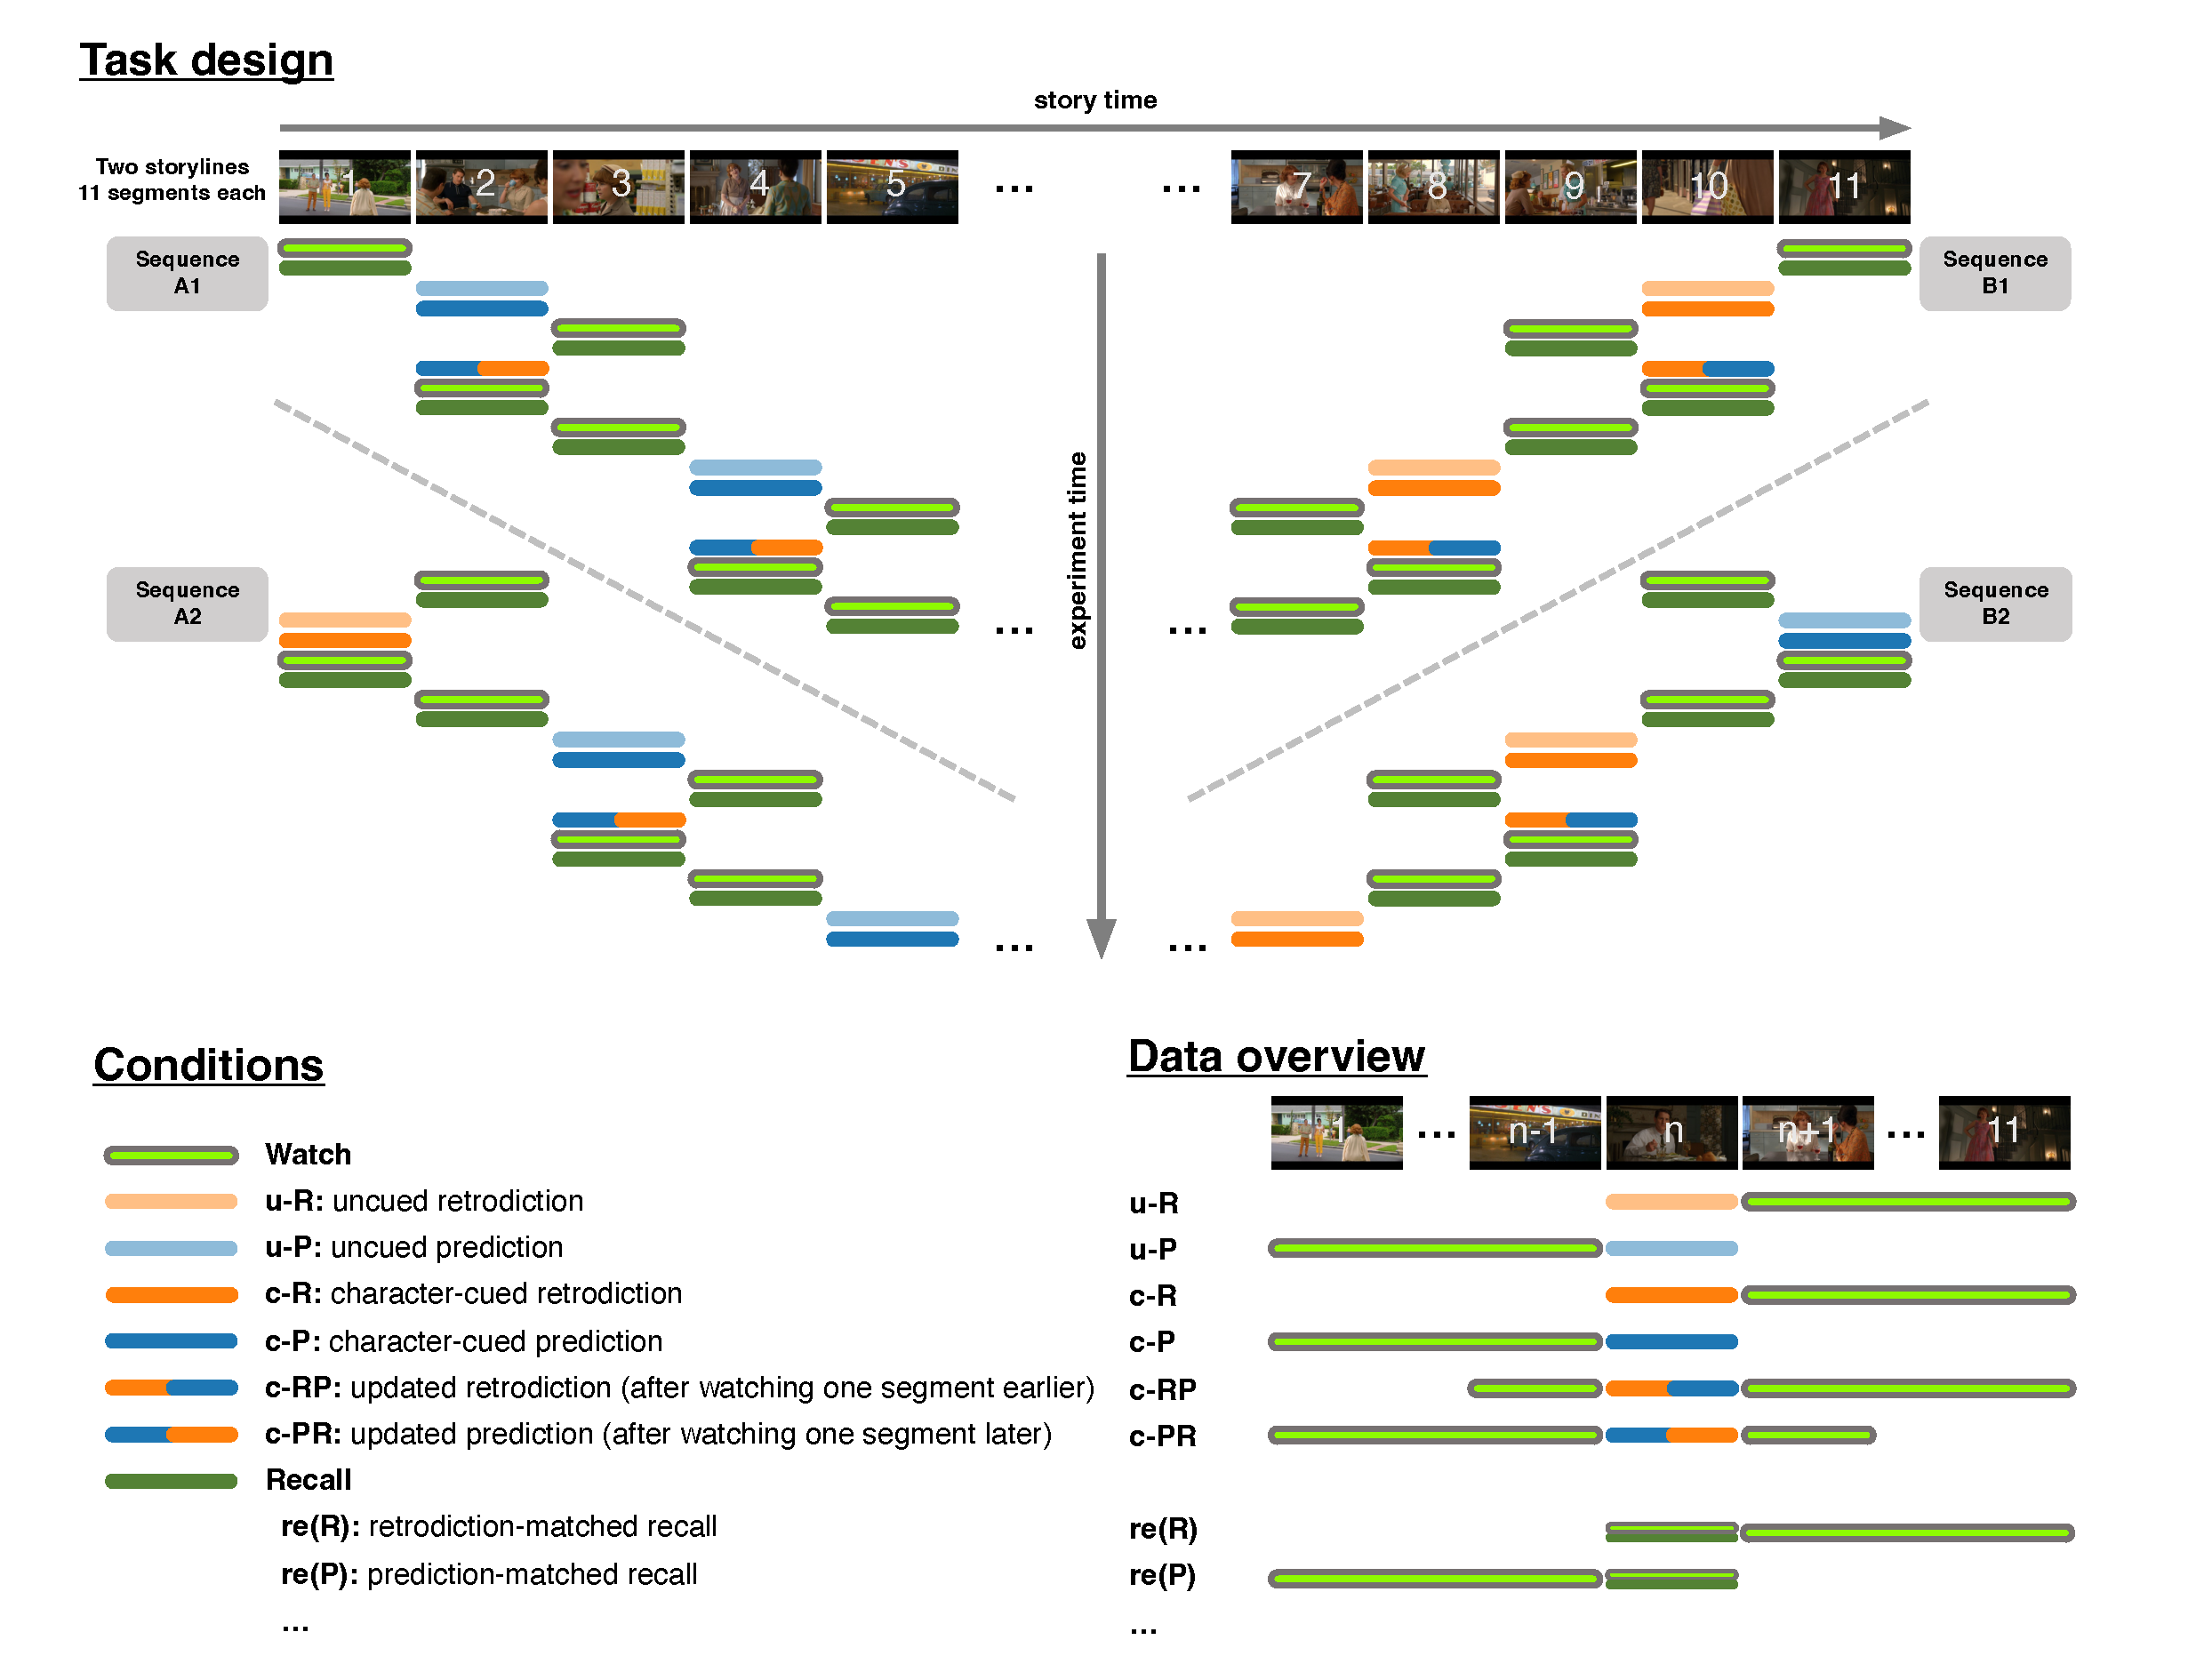
\includegraphics[width=\textwidth]{methods}
\DIFaddbeginFL 

  \DIFaddendFL \caption{\textbf{Task overview.} Participants \DIFaddbeginFL \DIFaddFL{in our main experiment }\DIFaddendFL watched segments of two storylines from the television series \textit{Why Women Kill}. They made free-form text responses to either retrodict what had happened in the previous segment, predict what would happen in the next segment, or recall what happened in the just-watched segment. Across four counterbalanced sequences, we systematically varied whether participants watched the segments in forward or reverse chronological order, whether (or not) responses were cued using the main characters in the target segment, and which other segments participants had watched prior to making a response. For each segment, we collected several retrodiction, prediction, and/or recall responses across different experimental conditions. \DIFaddbeginFL \DIFaddFL{Experiment time is denoted along the vertical axis, storyline segment orders are indicated along the horizontal axis, and the colors denote experimental tasks (conditions). For an analogous depiction of our replication experiment's design, see Fig.~\MethodsReplExp.}\DIFaddendFL }
\DIFaddbeginFL 

  \DIFaddendFL \label{fig:method}
\end{figure}

We asked participants \DIFaddbegin \DIFadd{in our main experiment }\DIFaddend to generate four types of responses after watching each video segment: uncued responses, character-cued responses, updated responses, and recalls (Fig.~\ref{fig:method}, \textit{Data overview}). To generate \textit{uncued} responses, we asked participants to either retrodict (uncued retrodiction; \textit{u-R}) what happened shortly before or predict (uncued prediction; \textit{u-P}) what happened shortly after the just-watched segment. To generate \textit{character-cued} responses, we asked participants to retrodict (character-cued retrodiction; \textit{c-R}) or predict (character-cued prediction; \textit{c-P}) what came before or after the just-watched segment, but we provided additional information to the participant about which character(s) would be present in the target (to-be-retrodicted or to-be-predicted) segment. We hypothesized that character-cued responses should be more accurate than uncued responses, to the extent that participants incorporate the character information we provided to them into their retrodictions and predictions. To generate updated responses, we asked participants to watch an additional segment that came just prior to or just after the target segment, and then to update their retrodiction (\textit{c-RP}) or prediction (\textit{c-PR}) about the target segment. Results on updated responses are not reported in this paper. Finally, we also asked participants to \textit{recall} what happened in the just-watched segment. We labeled these responses according to which other segments participants had watched prior to the just-watched target. Retrodiction-matched recall (\textit{re(R)}) responses were made during the retrodiction sequences (B1 and B2; Fig.~\ref{fig:method}), whereas prediction-matched recall (\textit{re(P)}) responses were made during the prediction sequences (A1 and A2\DIFdelbegin \DIFdel{).  Participants' recalls provided us with a benchmark for examining information about the participants' experiences and memories, without asking the participants to explicitly speculate about the unobserved.
}%DIFDELCMD < 

%DIFDELCMD < %%%
\DIFdel{For each }\DIFdelend \DIFaddbegin \DIFadd{; Fig.~\ref{fig:method}). Whereas }\DIFaddend retrodiction and prediction \DIFdelbegin \DIFdel{, participants were asked to generate at least one, and not more than three, responses that constituted ``the sorts of things }%DIFDELCMD < [%%%
\DIFdel{the participant would}%DIFDELCMD < ] %%%
\DIFdel{expect to have remembered if }%DIFDELCMD < [%%%
\DIFdel{they }%DIFDELCMD < ] %%%
\DIFdel{had watched the }%DIFDELCMD < [%%%
\DIFdel{target }%DIFDELCMD < ] %%%
\DIFdel{segment. ''  They were asked to generate multiple responses only if those additional responses were (in their judgement) of equal likelihood to occur.On average, participants generated 1.08 responses per prompt; therefore we chose to consider only participants' first (``most probable'' or ``most important'') responses to each prompt.  We also discarded a small number ($n = 20$) of character-cued responses that did not contain references to all cued characters, along with one additional response due to the participant's misunderstanding of the task instructions during that trial.  We carried out our analyses on the remaining 2084 retrodiction, prediction, and }\DIFdelend \DIFaddbegin \DIFadd{responses reflect what participants }\textit{\DIFadd{estimate}} \DIFadd{they would remember after watching the (inferred) target segment, recall responses provide a benchmark for comparison by measuring what they }\textit{\DIFadd{actually}} \DIFadd{remember about the target segment. Our replication experiment (Fig.~\MethodsReplExp) used a similar design, but did not have participants generate }\DIFaddend recall responses.


\begin{figure}[tp]
  \centering
  \DIFdelbeginFL %DIFDELCMD < 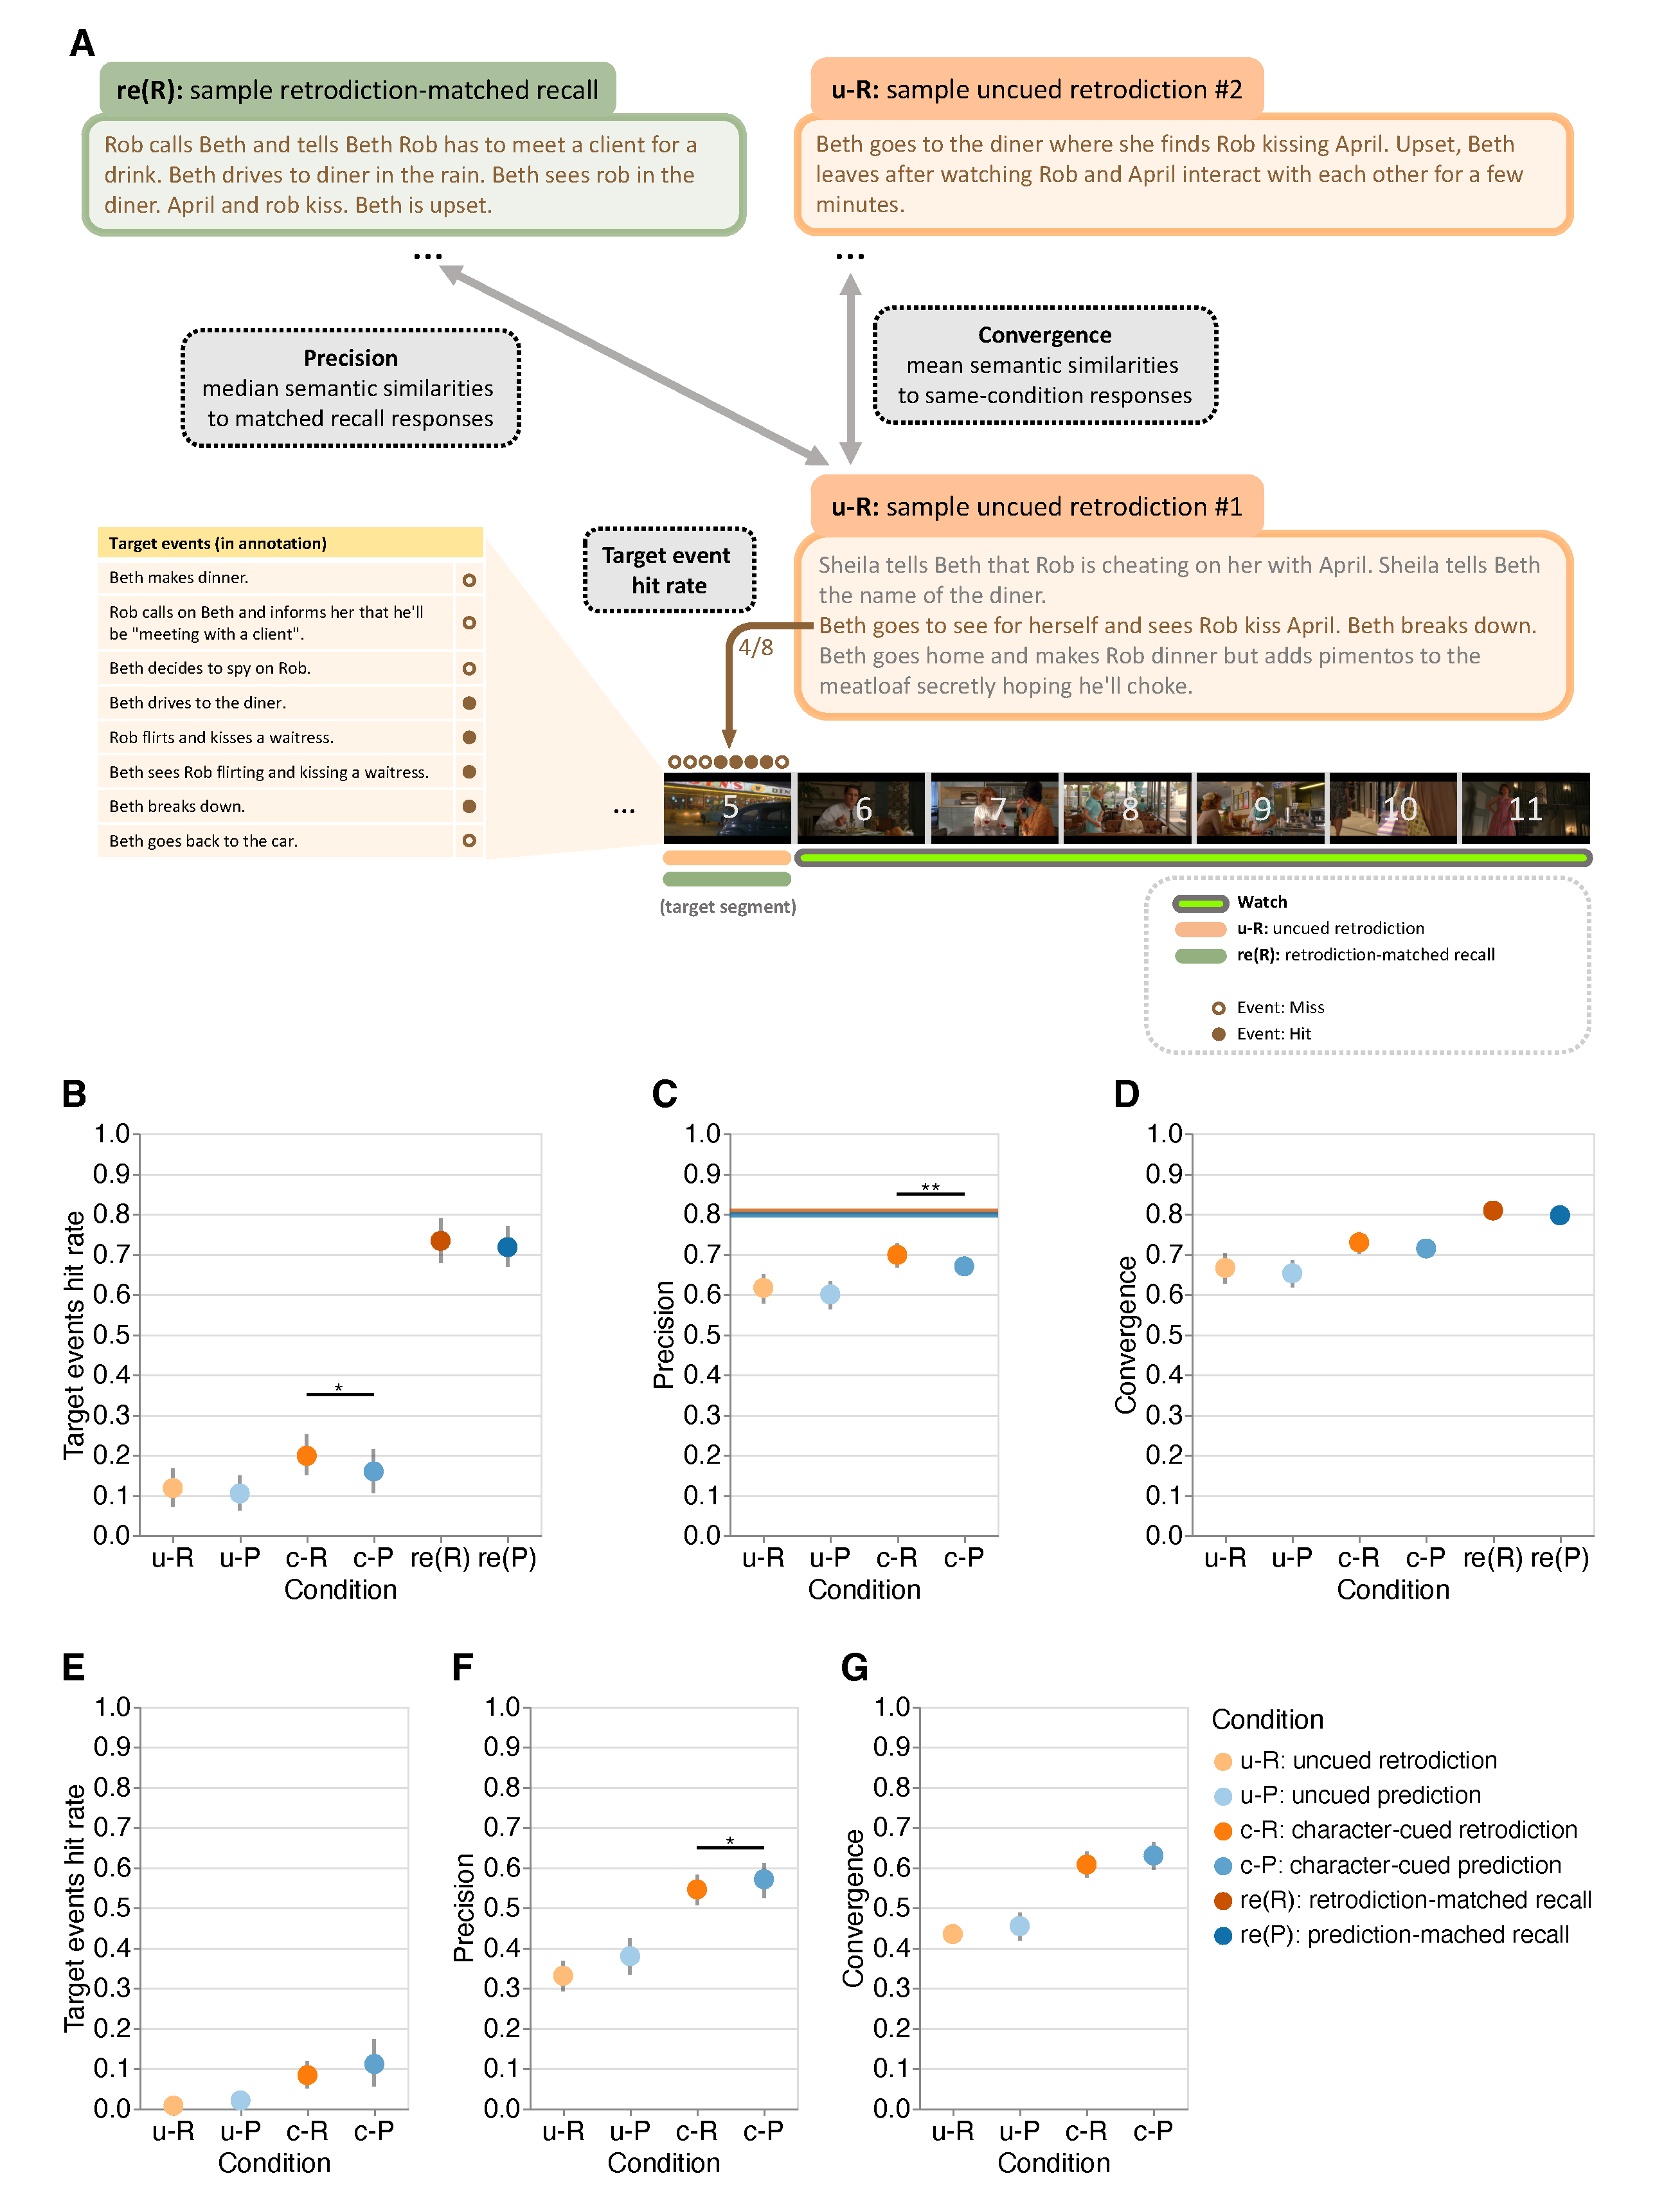
\includegraphics[width=0.80\textwidth]{results1}
%DIFDELCMD <   %%%
\DIFdelendFL \DIFaddbeginFL 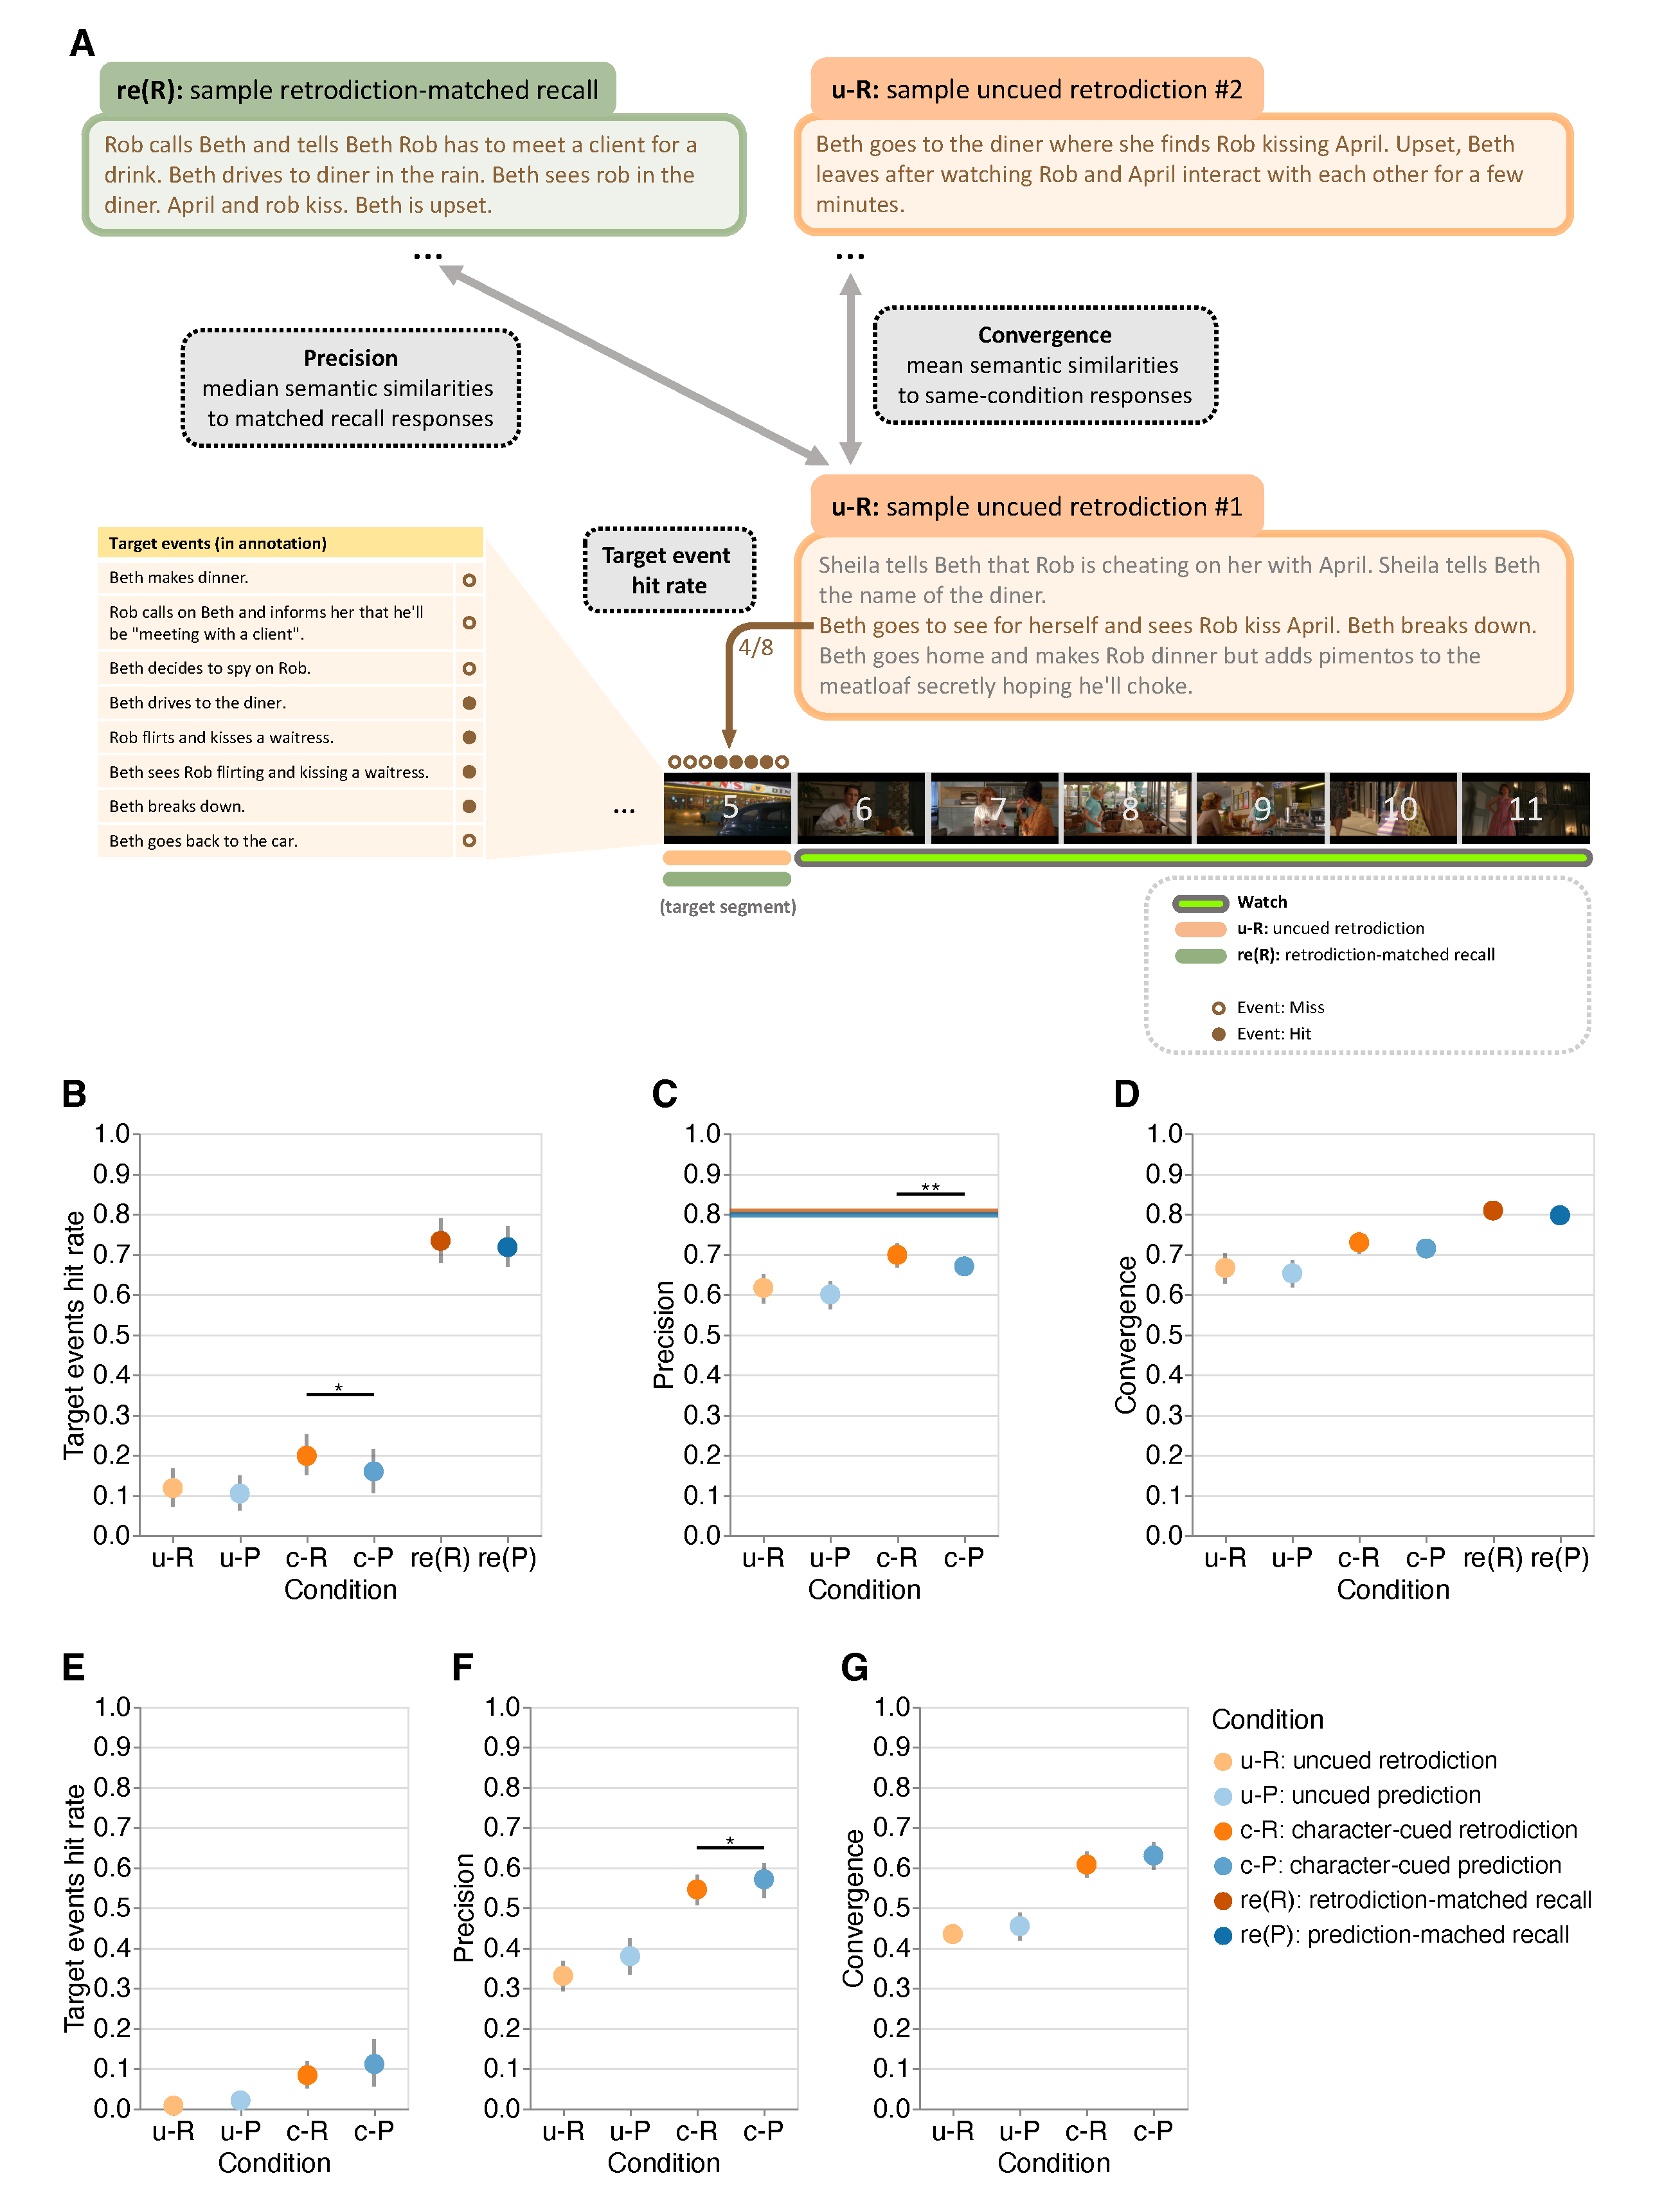
\includegraphics[width=0.7\textwidth]{results1}

  \DIFaddendFL \caption{\DIFdelbeginFL \textbf{\DIFdelFL{Retrodiction, prediction, and recall performance by experimental condition.}} %DIFAUXCMD
\DIFdelendFL \DIFaddbeginFL \textbf{\DIFaddFL{Retrodiction, prediction, and recall performance by experimental condition in our main and replication experiments.}} \DIFaddendFL \textbf{A. Methods schematic.} For each retrodiction, prediction, and recall response, we calculated the hit rate for events in the target segment \DIFaddbeginFL \DIFaddFL{(see }\textit{\DIFaddFL{Response analyses}}\DIFaddFL{)}\DIFaddendFL , the response precision (see \DIFdelbeginFL \textit{\DIFdelFL{Methods}}%DIFAUXCMD
\DIFdelendFL \DIFaddbeginFL \textit{\DIFaddFL{Text embeddings of participants’ responses}}\DIFaddendFL ), and the response convergence across participants\DIFdelbeginFL \DIFdelFL{(see }\textit{\DIFdelFL{Methods}}%DIFAUXCMD
\DIFdelFL{)}\DIFdelendFL . \DIFdelbeginFL \textbf{\DIFdelFL{B. Target event hit rate.}} %DIFAUXCMD
\DIFdelendFL \DIFaddbeginFL \textbf{\DIFaddFL{B. Target event hit rate (main experiment).}} \DIFaddendFL Mean proportions of target events that were contained in participants' responses, for each response type, averaged across target segments. \DIFdelbeginFL \textbf{\DIFdelFL{C. Response precision.}}  %DIFAUXCMD
\DIFdelendFL \DIFaddbeginFL \textbf{\DIFaddFL{C. Response precision (main experiment).}} \DIFaddendFL Mean precisions of participants' responses, for each response type, averaged across target segments. The horizontal lines denote the mean pairwise semantic similarities (see \DIFdelbeginFL \textit{\DIFdelFL{Methods}}%DIFAUXCMD
\DIFdelendFL \DIFaddbeginFL \textit{\DIFaddFL{Text embeddings of participants’ responses}}\DIFaddendFL ) across recall responses (re(R): orange; re(P): blue). \DIFdelbeginFL \textbf{\DIFdelFL{D. Response convergence.}}  %DIFAUXCMD
\DIFdelendFL \DIFaddbeginFL \textbf{\DIFaddFL{D. Response convergence (main experiment).}} \DIFaddendFL Mean (across-participant) convergence of participants' responses, for each response type, averaged across target segments. \DIFaddbeginFL \textbf{\DIFaddFL{E. Target event hit rate (replication experiment)}}\DIFaddFL{. Same format as Panel B. 
 }\textbf{\DIFaddFL{F. Response precision (replication experiment)}}\DIFaddFL{. Same format as Panel C.  }\textbf{\DIFaddFL{G. Response convergence (replication experiment)}}\DIFaddFL{. Same format as Panel D. }\DIFaddendFL All panels: error bars denote bootstrapped 95\% confidence intervals. Asterisks indicate significance in the (generalized) linear mixed models: * denotes $p < 0.05$ and ** denotes $p < 0.01$.}
\DIFaddbeginFL 

  \DIFaddendFL \label{fig:result1}
\end{figure}

We used two general approaches to assess the quality of participants' responses (see \textit{\DIFdelbegin \DIFdel{Methods}\DIFdelend \DIFaddbegin \DIFadd{Response analyses, Text embeddings of participants’ responses}\DIFaddend }, Fig.~\ref{fig:result1}A). One approach entailed manually annotating events in the video and counting the number of matched events in participants' responses. We identified a total of 117 unique events reflected across the 22 video segments \DIFaddbegin \DIFadd{in our main experiment }\DIFaddend (range: 3--9 per segment\DIFdelbegin \DIFdel{; see }\DIFdelend \DIFaddbegin \DIFadd{), and a total of 71 events across the 13 segments in our replication experiment (range 1--16; see }\DIFaddend \textit{\DIFdelbegin \DIFdel{Methods}\DIFdelend \DIFaddbegin \DIFadd{Video annotation}\DIFaddend }, \DIFdelbegin \DIFdel{Table \stimDescription}\DIFdelend \DIFaddbegin \DIFadd{Tables~\stimDescription,~\stimDescriptionRep}\DIFaddend ). We assigned one ``point'' to each of these video events. We also identified \DIFdelbegin \DIFdel{23 additional events }\DIFdelend \DIFaddbegin \DIFadd{a number of additional events (main experiment: 23; replication experiment: 17) }\DIFaddend in participants' responses that were either summaries of several events or that were partial matches to the manually identified video events. We assigned 0.5 point to each of these additional events. This point system enabled us to compute the numbers and proportions (\textit{hit rates}) of correctly retrodicted, predicted, and recalled events contained in each response. Our second approach entailed using a natural language processing model~\citep{CerEtal18} to embed annotations and responses in a 512-dimensional feature space. This approach was designed to capture conceptual overlap between responses that were not necessarily tied to specific events. To quantify this conceptual overlap, we computed the similarities between the embeddings of different sets of responses. Following \cite{HeusEtal21}, we defined the \textit{precision} of \DIFdelbegin \DIFdel{each participants' retrodictions or predictions about a given segment }\DIFdelend \DIFaddbegin \DIFadd{participants' responses }\DIFaddend as the median cosine \DIFdelbegin \DIFdel{similarities between }\DIFdelend \DIFaddbegin \DIFadd{similarity between that response's vector and the embedding vectors for all other participants' recalls of the target segment (main experiment), or the similarity between that response's vector and the embedding vector for an online plot synopsis (obtained via Screen Spy; }\url{www.screenspy.com/the-chair-season-1-episode-1}\DIFadd{) of }\DIFaddend the \DIFdelbegin \DIFdel{embeddings of (a)the participant's retrodiction or prediction response for the given segment and (b) each }\textit{\DIFdel{other}} %DIFAUXCMD
\DIFdel{participant's recalls of the same segment }\DIFdelend \DIFaddbegin \DIFadd{target segment (replication experiment)}\DIFaddend .  In other words, precision is designed to measure the extent to which retrodictions and predictions captured the conceptual content that (other) participants remembered. We also developed a related measure, which we call \textit{convergence}, to characterize response similarities across participants. In particular, we defined convergence as the mean cosine similarity between the embeddings of a participant's responses to a \DIFdelbegin \DIFdel{given }\DIFdelend target segment and all other participants' responses (of the same type) to the same segment. We analyzed the data using generalized linear mixed models, with participant and stimulus (e.g., target segment) identities as crossed random effects (see \textit{\DIFdelbegin \DIFdel{Methods}\DIFdelend \DIFaddbegin \DIFadd{Statistical analysis}\DIFaddend }).

First we sought to validate a main effect of response type (i.e., uncued responses, character-cued responses, and recalls), irrespective of the temporal direction (retrodiction versus prediction). Across these three types of responses, participants have access to increasing amounts of information about the target segment. Therefore, across these response types, we hypothesized that participants' responses should become both more accurate and more convergent across individuals. Consistent with this hypothesis, participants' character-cued retrodictions and predictions were associated with higher target event hit rates than uncued retrodictions and predictions \DIFaddbegin \DIFadd{in our main experiment }\DIFaddend (odds ratio (OR): 2.65, $Z = 4.24$, $p < 0.001$, 95\% confidence interval (CI): 1.69 to 4.16; Fig.~\ref{fig:result1}B). These character-cued responses were also more precise ($b = 0.13$, $t(18.1) = 9.43$, $p < 0.001$, CI: 0.10 to 0.16; Fig.~\ref{fig:result1}C) and convergent across individuals ($b = 0.11$, $t(18.6) = 6.21$, $p < 0.001$, CI: 0.07 to 0.15; Fig.~\ref{fig:result1}D). Relative to character-cued responses, participants' recalls showed higher target event hit rates (OR = 21.83, $Z = 10.61$, $p < 0.001$, CI: 12.35 to 38.59) and \DIFaddbegin \DIFadd{were }\DIFaddend more convergence across individuals ($b = 0.20$, $t(19.4) = 9.10$, $p < 0.001$, CI: 0.16 to 0.25). These results are consistent with the common-sense notion that access to more information about a target segment yields better performance (i.e., higher hit rates, precision, and convergence across individuals).  \DIFaddbegin \DIFadd{These findings also held for our replication experiment (target event hit rates of character-cued vs. uncued responses: OR: 18.63, $Z = 4.26$, $p < 0.001$, CI: 4.85 to 71.58, Fig.~\ref{fig:result1}E; precisions of character-cued vs. uncued responses: $b = 0.26$, $t(11.70) = 9.87$, $p < 0.001$, CI: 0.20 to 0.31, Fig.~\ref{fig:result1}F; convergence of character-cued vs. uncued responses: $b = 0.25$, $t(11.98) = 8.93$, $p < 0.001$, CI: 0.19 to 0.31, Fig.~\ref{fig:result1}G).
}\DIFaddend 

Next we carried out a series of analyses specifically aimed at characterizing temporal direction effects--- i.e, the relative quality of retrodictions versus predictions across different types of responses. We hoped that these analyses might provide insights into our central question about whether \DIFdelbegin \DIFdel{the present is equally informative }\DIFdelend \DIFaddbegin \DIFadd{inferences }\DIFaddend about the past and future \DIFaddbegin \DIFadd{are equally accurate}\DIFaddend . Across both uncued and character-cued responses \DIFaddbegin \DIFadd{in our main experiment }\DIFaddend (Fig.~\ref{fig:method}), retrodictions had numerically higher hit rates than predictions (Fig.~\ref{fig:result1}B). However, these differences were only statistically reliable for character-cued responses (uncued responses: OR = 1.17, $Z = 0.35$, $p = 0.73$, CI: 0.47 to 2.92; character-cued responses: OR = 1.93, $Z = 2.15$, $p = 0.03$, CI: 1.06 to 3.52). We observed a similar pattern of results for the precisions of participants' responses (Fig.~\ref{fig:result1}C). Specifically, their responses tended to be numerically more precise for retrodictions versus predictions, but the differences were only statistically reliable for character-cued responses (uncued responses: $b = 0.03$, $t(20.9) = 1.09$, $p = 0.29$, CI: -0.03 to 0.10; character-cued responses: $b = 0.06$, $t(20.8) = 3.01$, $p = 0.007$, CI: 0.02 to 0.11). We also consistently observed numerically higher convergence across participants for retrodictions versus predictions (Fig.~\ref{fig:result1}D), but neither of these differences were statistically reliable (uncued responses: $b = 0.03$, $t(17.9) = 0.75$, $p = 0.46$, CI: -0.05 to 0.11; character-cued responses: $b = 0.04$, $t(17.4) = 1.46$, $p = 0.16$, CI: -0.02 to 0.09).  \DIFdelbegin \DIFdel{Because the retrodiction versus prediction performance differences we observed were only statistically reliable when participants were cued with the target segments' characters, this suggests that information about the unobserved past versus the unobserved future may differently affect retrodictions versus predictions.  Taken together, these results suggest that participants are generally better at making retrodictions than predictions.  We also verified that this was not solely a consequence of how participants' memory performance might have been affected by watching different segments (or making different responses to other segments) across conditions by comparing recall responses in the retrodiction-matched recall (}\textit{\DIFdel{re(R)}}%DIFAUXCMD
\DIFdel{) and prediction-matched recall (}\textit{\DIFdel{re(P)}}%DIFAUXCMD
\DIFdel{) conditions.  Recall performance was similar in both conditions (}\DIFdelend \DIFaddbegin \DIFadd{In our replication experiment, as in our main experiment, most of these differences were not statistically reliable (target event hit rates for uncued responses: OR = 0.11, $Z = -1.92$, $p = 0.05$, CI: 0.01 to 1.04; }\DIFaddend target event hit \DIFdelbegin \DIFdel{rate}\DIFdelend \DIFaddbegin \DIFadd{rates for character-cued responses}\DIFaddend : OR = \DIFdelbegin \DIFdel{1.12, $Z = 1.07$, $p = 0.29$}\DIFdelend \DIFaddbegin \DIFadd{1.42, $Z = 0.62$, $p = 0.53$}\DIFaddend , CI: \DIFdelbegin \DIFdel{0.91 to 1.39; convergence: $b = 0.03$, $t(19.3) = 1.89$, $p = 0.07$}\DIFdelend \DIFaddbegin \DIFadd{0.47 to 4.23, Fig.~\ref{fig:result1}E; precision for uncued response: $b = -0.06$, $t(15.86) = -1.85$, $p = 0.08$}\DIFaddend , CI: \DIFaddbegin \DIFadd{-0.12 to 0.01; precision for character-cued responses: $b = -0.04$, $t(25.02) = -2.28$, $p = 0.03$, CI: -0.08 to }\DIFaddend 0.00\DIFaddbegin \DIFadd{, Fig.~\ref{fig:result1}F; convergence for uncued responses: $b = -0.03$, $t(12.15) = -0.55$, $p = 0.59$, CI: -0.13 }\DIFaddend to 0.07\DIFdelbegin \DIFdel{).
}\DIFdelend \DIFaddbegin \DIFadd{; convergence for character-cued responses: $b = -0.05$, $t(13.68) = -1.78$, $p = 0.10$, CI: -0.11 to 0.01, Fig.~\ref{fig:result1}G).  Taken together, our results from both experiments suggest that participants’ inferences about the immediate past and future do }\textit{\DIFadd{not}} \DIFadd{show reliable asymmetries.
}\DIFaddend 

\begin{figure}[tp]
  \centering
  \DIFdelbeginFL %DIFDELCMD < 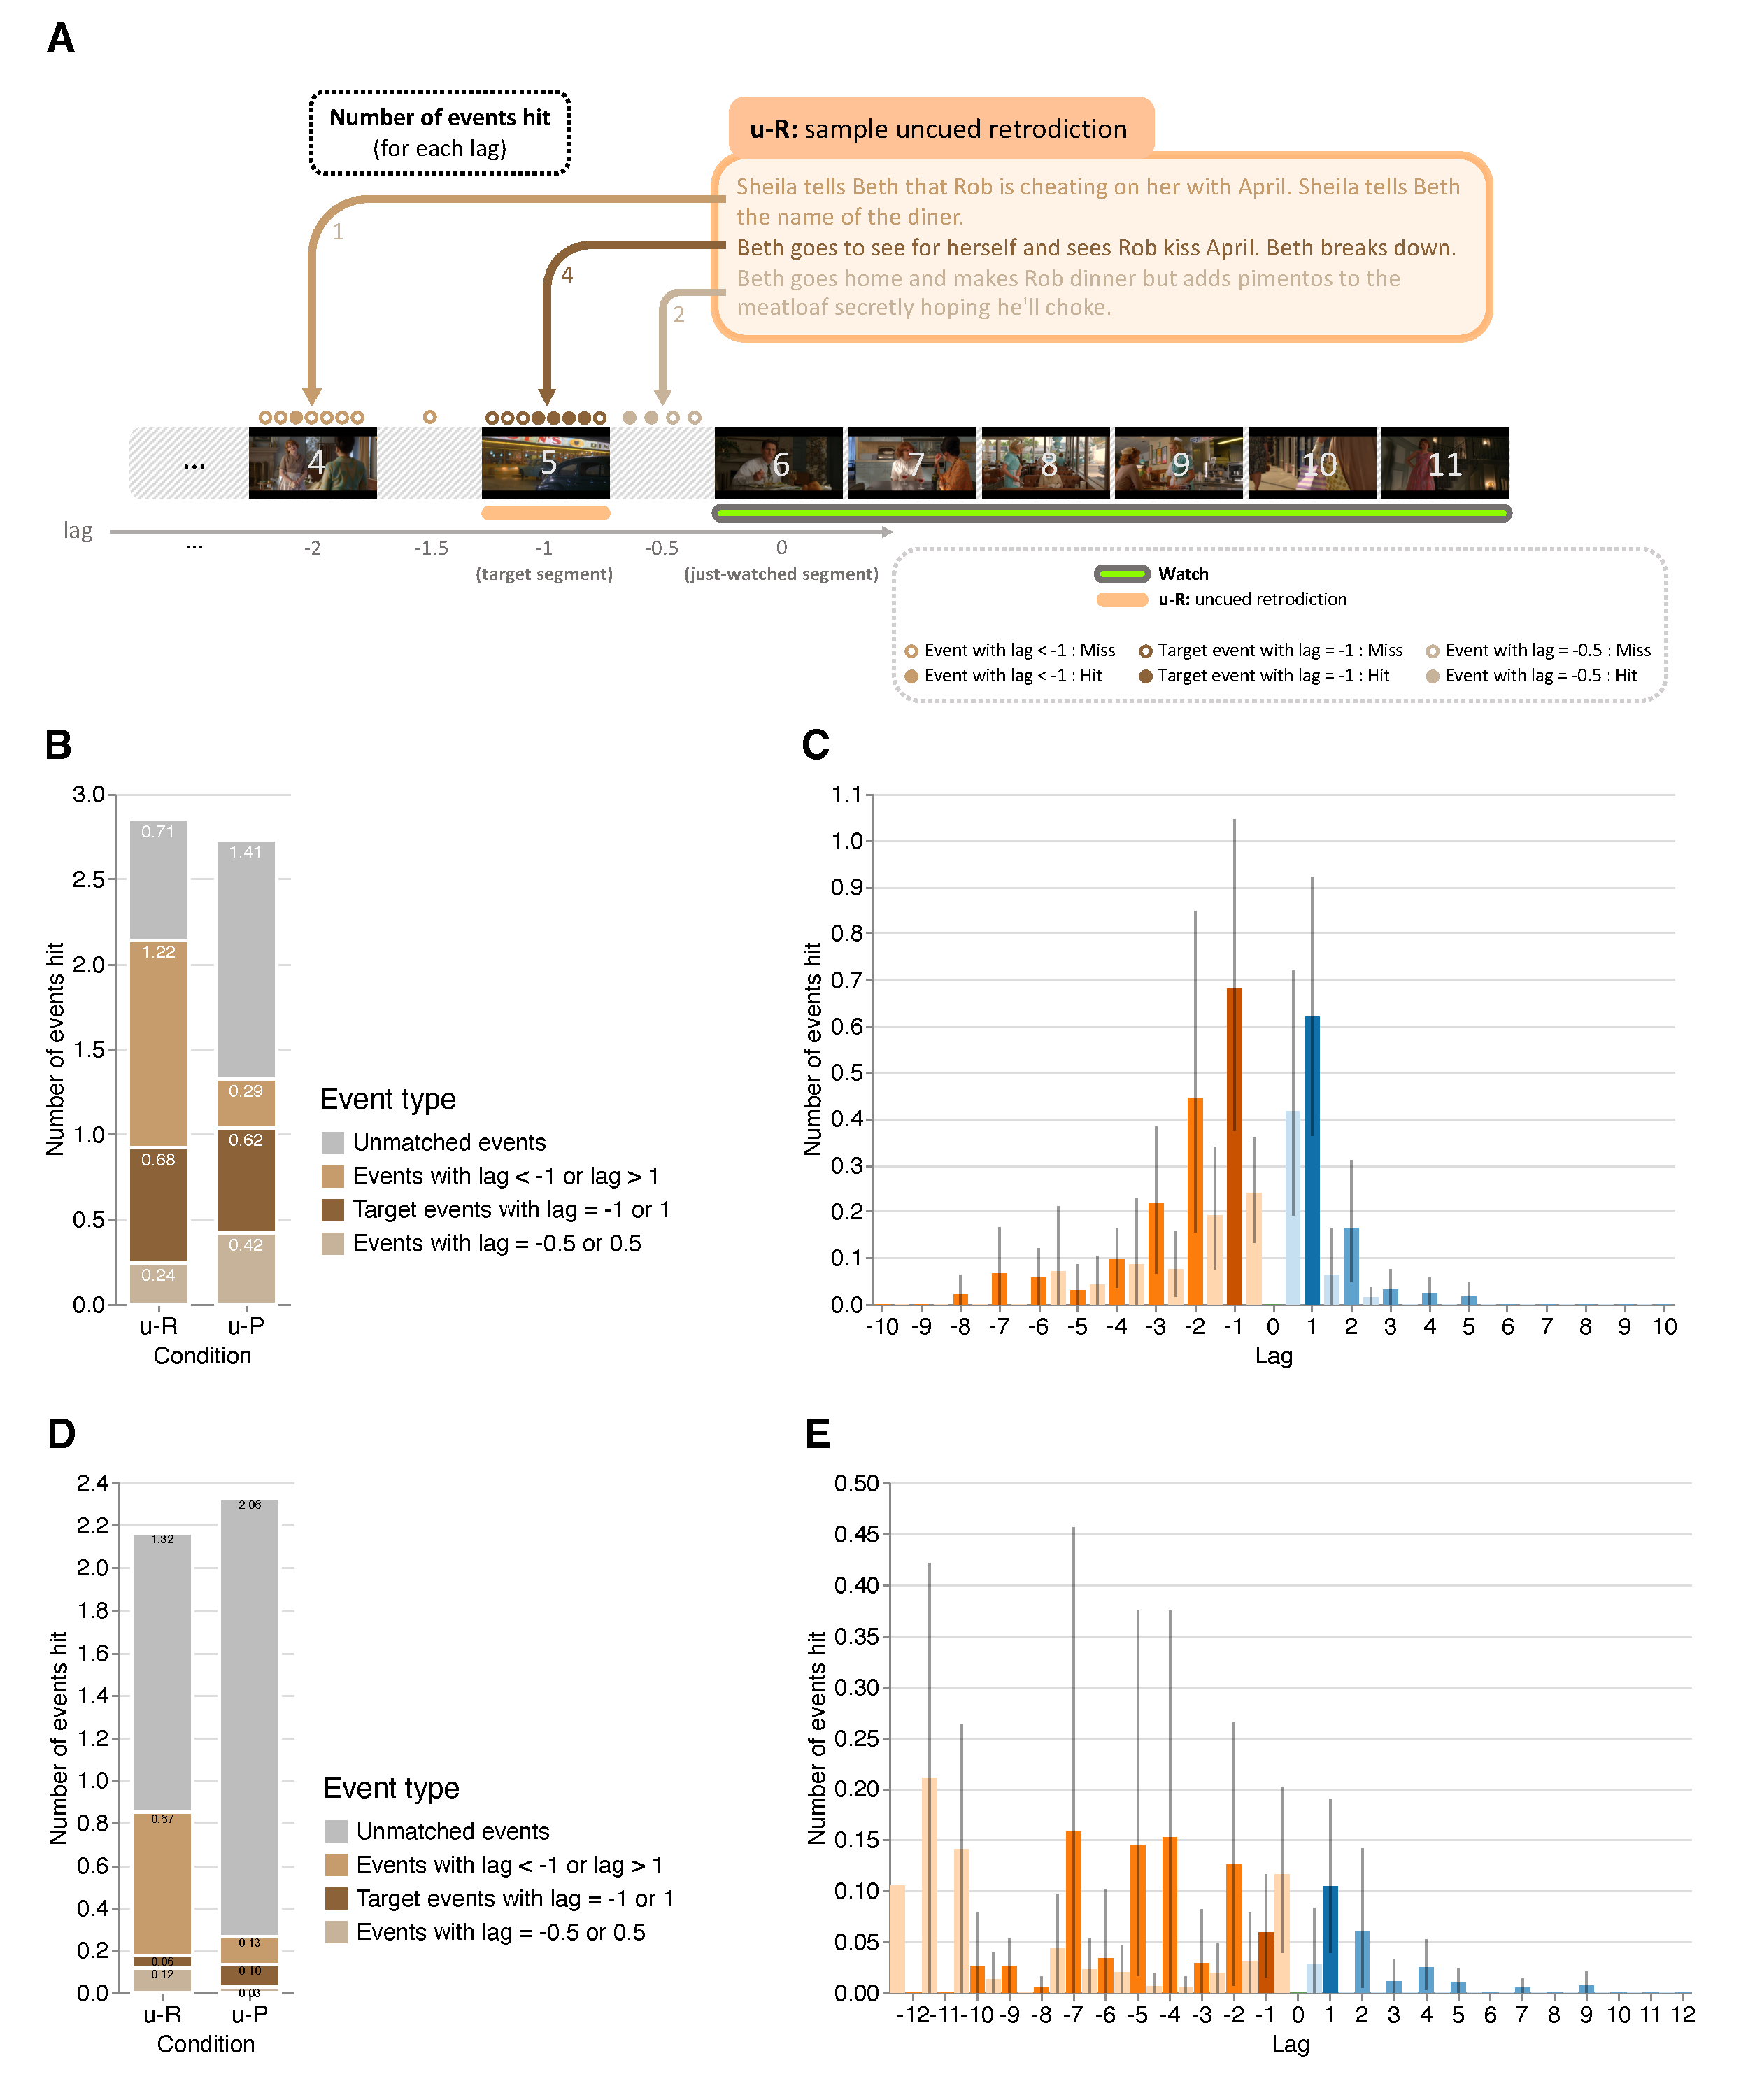
\includegraphics[width=\textwidth]{results2}
%DIFDELCMD <   %%%
\DIFdelendFL \DIFaddbeginFL 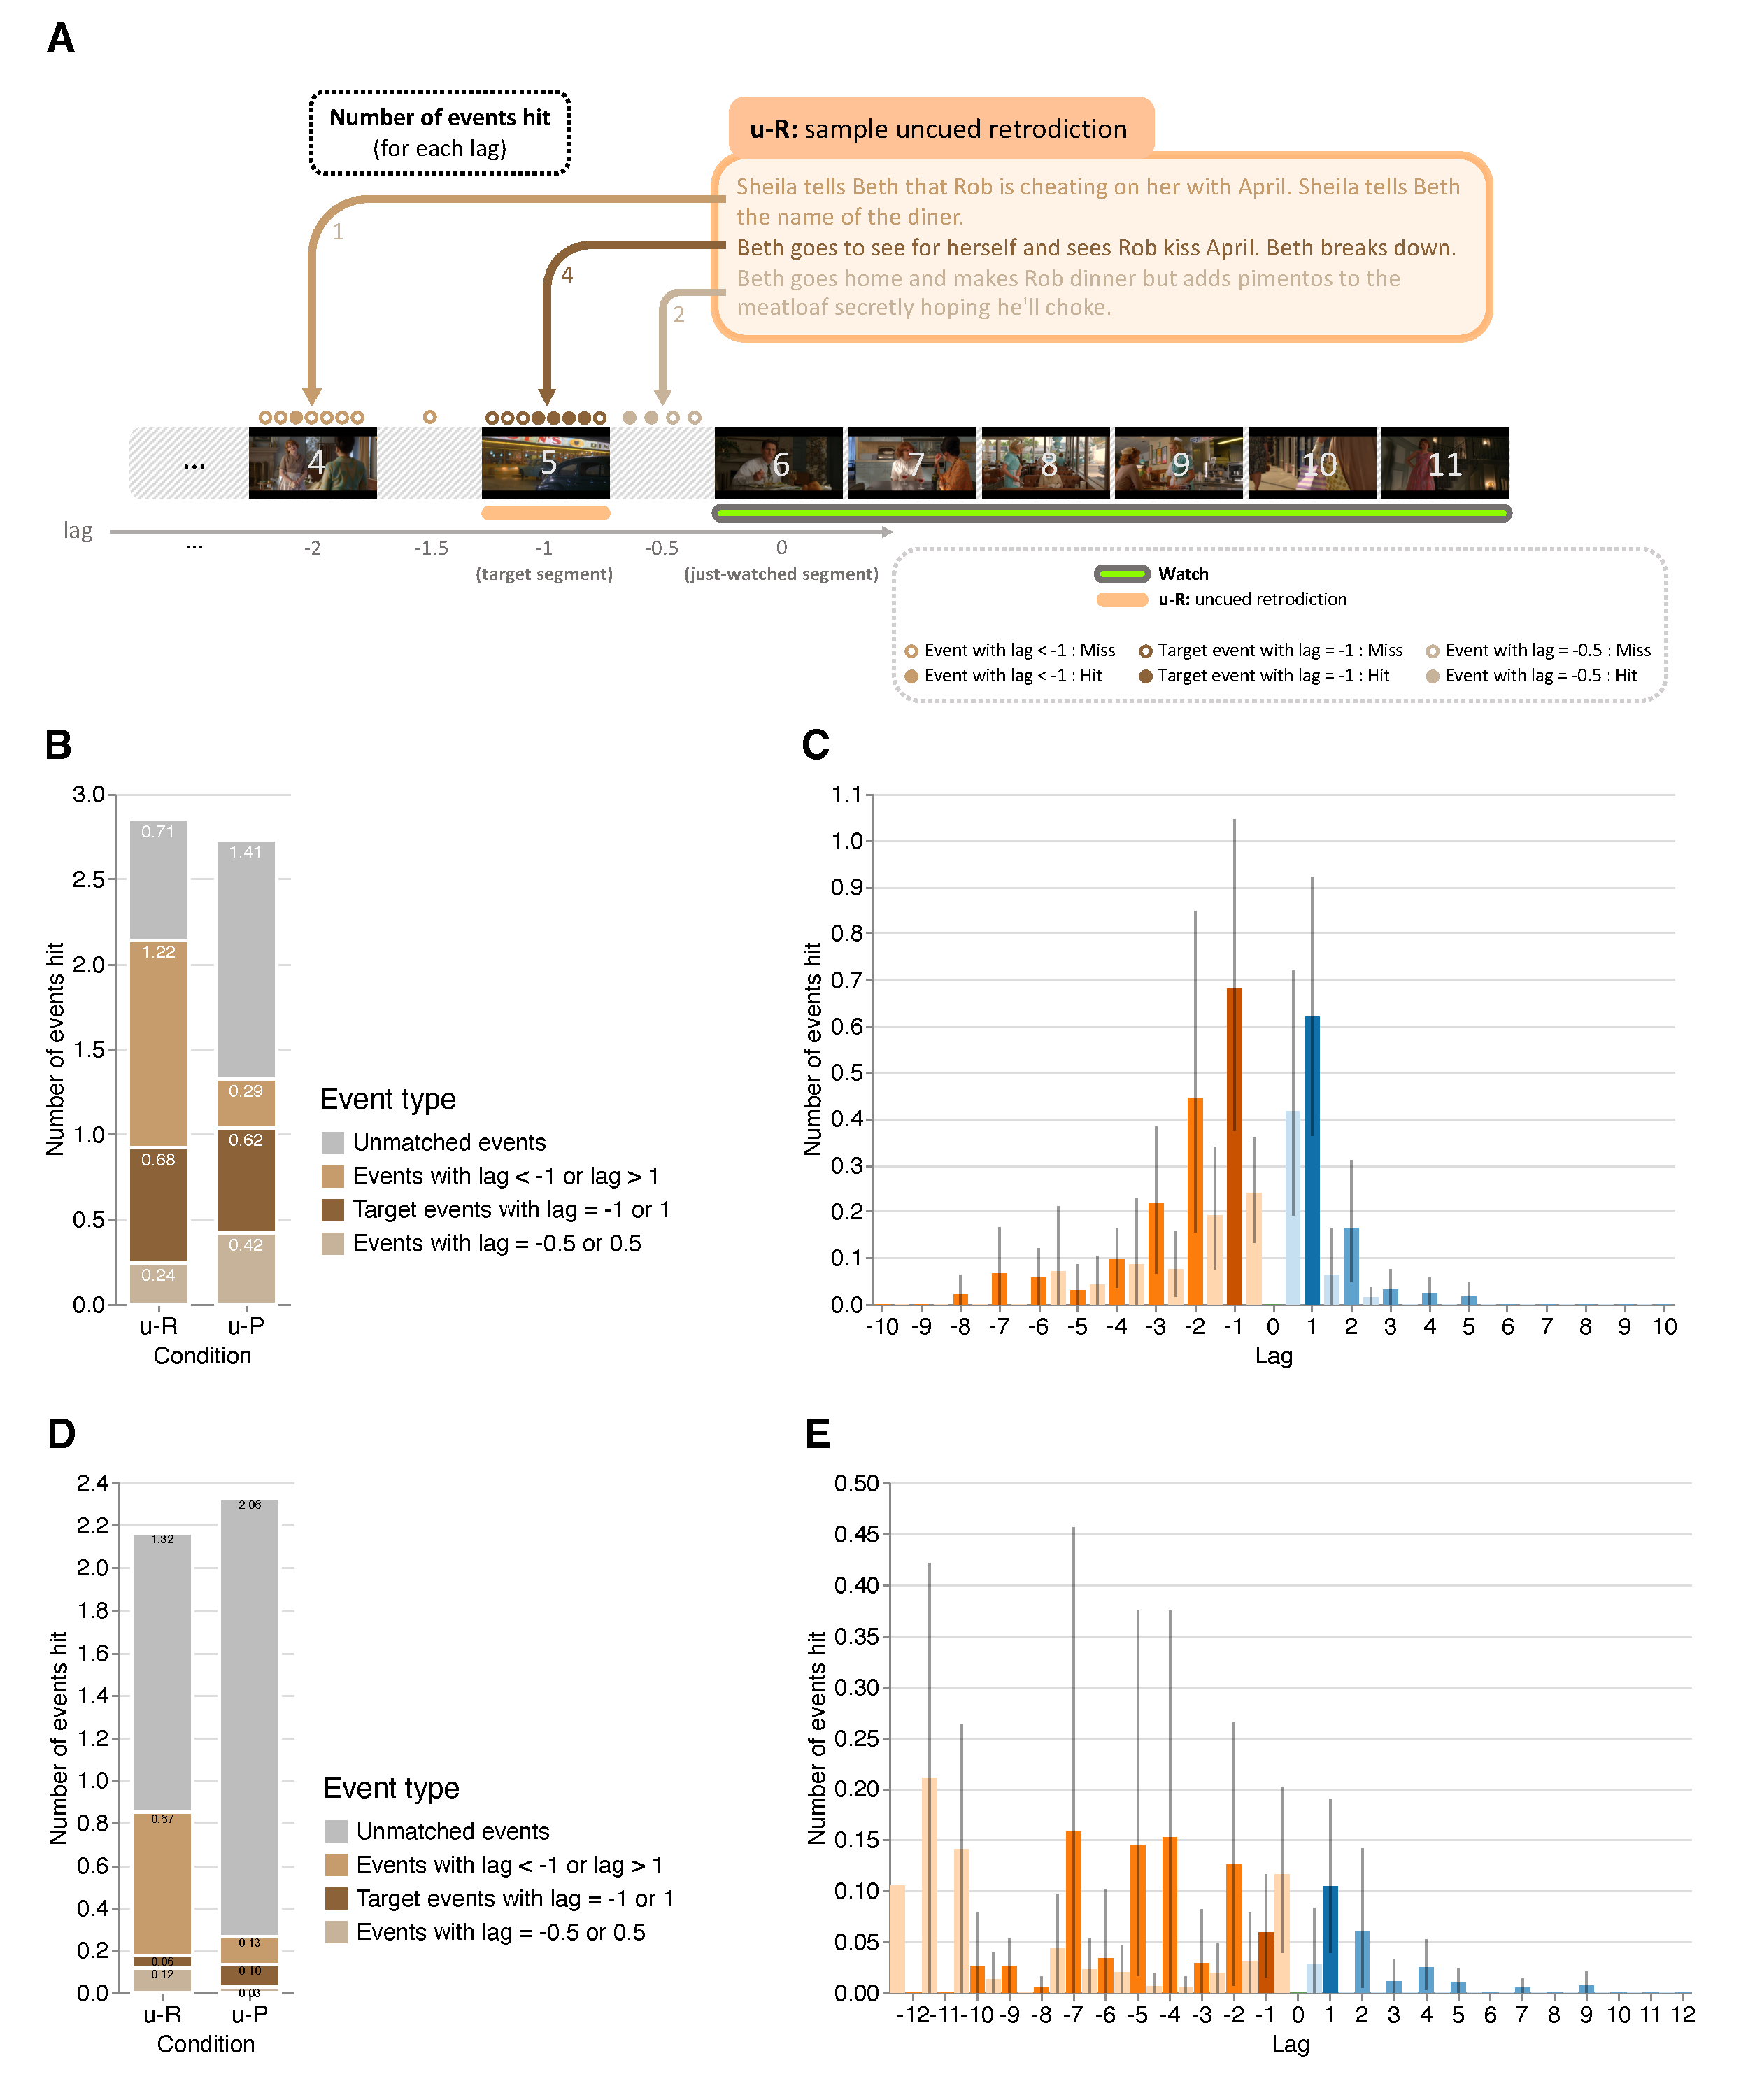
\includegraphics[width=0.7\textwidth]{results2}

  \DIFaddendFL \caption{\textbf{Retrodictions and predictions of temporally near and distant events.} \textbf{A. Illustration of annotation approach.} For each uncued retrodiction and prediction response, we calculated the number of (retrodicted or predicted) events as a function of temporal distance from the target segment, or \textit{lag}. Onscreen (explicit) events are tagged using integer-valued lags, whereas offscreen (implicit) events are tagged using half-step lags ($\pm 0.5$, $\pm 1.5$, etc.). \DIFdelbeginFL \textbf{\DIFdelFL{B. Number of events hit in participants' uncued retrodictions and predictions for each event type.}}  %DIFAUXCMD
\DIFdelendFL \DIFaddbeginFL \textbf{\DIFaddFL{B. Number of events hit in participants' uncued retrodictions and predictions for each event type (main experiment).}} \DIFaddendFL Here we separated events we identified in participants' responses according to whether they occurred in the target segment (lags of $\pm 1$), during the interval between the target segment and the just-watched segment (lags of $\pm 0.5$), at longer temporal distances ($|\mathrm{lag}| > 1$), or were incorrect (unmatched with any past or future events in the narrative). The counts displayed in the panel are averaged across just-watched segments. \DIFdelbeginFL \textbf{\DIFdelFL{C. Number of events hit as a function of temporal distance.}}  %DIFAUXCMD
\DIFdelendFL \DIFaddbeginFL \textbf{\DIFaddFL{C. Number of events hit as a function of temporal distance (main experiment).}} \DIFaddendFL Here the (across-segment) mean numbers of events hit in participants' uncued retrodictions (orange) and predictions (blue) are displayed as a function of temporal distance to the just-watched segment (lag). \DIFaddbeginFL \textbf{\DIFaddFL{D. Number of events hit in participants' uncued retrodictions and predictions for each event type (replication experiment).}} \DIFaddFL{Same format as Panel B.  }\textbf{\DIFaddFL{E. Number of events hit as a function of temporal distance (replication experiment).}} \DIFaddFL{Same format as Panel C.  }\DIFaddendFL Error bars denote bootstrapped 95\% confidence intervals. Colors denote temporal direction (orange: past; blue: future) and distance (darker shading: onscreen events from segments adjacent to the target segment; lighter shading: offscreen events).}
\DIFaddbeginFL 

  \DIFaddendFL \label{fig:result2}
\end{figure}

The above analyses were focused solely on the target segment (i.e., retrodiction of segment \DIFdelbegin \DIFdel{$i - 1$ }\DIFdelend \DIFaddbegin \DIFadd{$n$ }\DIFaddend after watching segments \DIFdelbegin \DIFdel{$i...11$}\DIFdelend \DIFaddbegin \DIFadd{$(n+1)...N$}\DIFaddend , or prediction of segment \DIFdelbegin \DIFdel{$i + 1$ }\DIFdelend \DIFaddbegin \DIFadd{$n$ }\DIFaddend after watching segments \DIFdelbegin \DIFdel{$1...i$}\DIFdelend \DIFaddbegin \DIFadd{$1 ...(n-1)$}\DIFaddend ). We wondered whether participants' responses might also contain longer-range information about preceding or proceeding events. In order to carry out this analysis properly, we reasoned that participants might reference past or future events that were \textit{implied} to have occurred offscreen, but not explicitly shown onscreen. For example, a character in location A during one scene might appear in location B during the immediately following scene. Although it wasn't shown onscreen, we can infer that the character traveled between locations A and B sometime between the time intervals separating the scenes~\citep{Bord08}. In all, we manually identified a set of 74 \textit{implicit} offscreen events \DIFaddbegin \DIFadd{in our main experiment's stimuli }\DIFaddend that were implied to have occurred given what was (explicitly) depicted onscreen (Fig.~\ref{fig:result2}A), plus one additional partial event and one additional summary event. We \DIFaddbegin \DIFadd{applied the same procedure to our replication experiment's stimuli and identified 66 implicit offscreen events, plus two additional partial events and one additional summary event. We }\DIFaddend defined the just-watched segment as having a \textit{lag} of 0. We assigned the target segment of a participant's retrodiction or prediction (i.e., the immediately preceding or proceeding segment) a lag of -1 or +1, respectively. The segment following the next was assigned a lag of \DIFaddbegin \DIFadd{+}\DIFaddend 2, and so on. We tagged offscreen events using half steps. For example, an offscreen event that occurred after the prior segment but before the just-watched segment would be assigned a lag of -0.5.

Because there is no ``ground truth'' number of offscreen events, we could not compute the hit rates for offscreen events. Instead, we counted up the absolute \textit{number} of retrodicted or predicted events as a function of lag. In other words, given that the participant had just watched segment $i$, we asked how many events from segment $i + lag$ they retrodicted or predicted, on average, given that they were aiming to retrodict or predict events at lags of $\pm 1$. We also counted the numbers of \textit{unmatched} events in participants' responses that did not correspond to any events in the relevant segments of the narrative. We focused specifically on \textit{uncued} retrodictions and predictions, which we hypothesized would provide the cleanest characterizations of participants' initial estimates of the unobserved past and future (i.e., without potential biases introduced by additional character information, as in the character-cued responses).  \DIFdelbegin \DIFdel{The }\DIFdelend \DIFaddbegin \DIFadd{For participants in our main experiment, the }\DIFaddend numbers of uncued retrodicted and predicted target (lag = \DIFdelbegin \DIFdel{$\pm 1$}\DIFdelend \DIFaddbegin \DIFadd{$\pm1$}\DIFaddend ) events were not reliably different (\DIFdelbegin \DIFdel{OR }\DIFdelend \DIFaddbegin \DIFadd{Ratio }\DIFaddend = 0.92, $Z = -0.15$, $p = 0.88$, CI: 0.30 to 2.84\DIFaddbegin \DIFadd{; Fig.~\ref{fig:result2}B}\DIFaddend ). In other words, uncued retrodictions and predictions over short timescales did not exhibit reliable asymmetries. \DIFaddbegin \DIFadd{This ``null result'' also held in our replication experiment (Ratio = 0.44, $Z = -1.38$, $p = 0.17$, CI: 0.14 to 1.41; Fig.~\ref{fig:result2}D). }\DIFaddend However, when retrodicting, participants \DIFaddbegin \DIFadd{in both experiments }\DIFaddend mentioned events from the distant past ($\mathrm{lag} < -1$) more often than participants predicted events from the distant future ($\mathrm{lag} > 1$; \DIFdelbegin \DIFdel{OR }\DIFdelend \DIFaddbegin \DIFadd{main experiment: Ratio }\DIFaddend = 9.10, $Z = 3.80$, $p < 0.001$, CI: 2.92 to 28.39; Fig.~\ref{fig:result2}B, C; \DIFaddbegin \DIFadd{replication experiment:Ratio = 7.98, $Z = 5.50$, $p < 0.001$, CI: 3.81 to 16.74; Fig.~\ref{fig:result2}D, E; }\DIFaddend for results from the character-cued conditions, see \DIFdelbegin \DIFdel{Fig.~}%DIFDELCMD < \events%%%
\DIFdelend \DIFaddbegin \DIFadd{Figs.~\stackedbar,~\stackedbarRep}\DIFaddend ). Despite this asymmetry in the \DIFdelbegin \DIFdel{accuracies }\DIFdelend \DIFaddbegin \DIFadd{accuracy }\DIFaddend of participants' long-range retrodictions versus predictions, there were no reliable differences in the \textit{\DIFdelbegin \DIFdel{numbers}\DIFdelend \DIFaddbegin \DIFadd{total}\DIFaddend } \DIFaddbegin \DIFadd{numbers }\DIFaddend of uncued retrodicted versus predicted events (\DIFdelbegin \DIFdel{across all lags; OR }\DIFdelend \DIFaddbegin \DIFadd{main experiment: Ratio }\DIFaddend = 1.05, $Z = 0.75$, $p = 0.45$, CI: 0.93 to 1.18\DIFdelbegin \DIFdel{).  Nor did we }\DIFdelend \DIFaddbegin \DIFadd{; replication experiment: Ratio = 0.93, $Z = -0.67$, $p = 0.50$, CI: 0.75 to 1.15). We did not }\DIFaddend find any reliable differences in the numbers of offscreen events immediately before or after the just-watched segment \DIFaddbegin \DIFadd{in our main experiment }\DIFaddend ($lag = \pm 0.5$; \DIFdelbegin \DIFdel{OR }\DIFdelend \DIFaddbegin \DIFadd{main experiment: Ratio }\DIFaddend = 0.75, $Z = -0.36$, $p = 0.72$, CI: 0.15 to 3.59)\DIFaddbegin \DIFadd{, but participants in our replication experiment responded with more prior (versus future) immediate offscreen events (Ratio = 26.46, $Z = 2.45$, $p = 0.01$, CI: 1.93 to 362.29)}\DIFaddend . The apparent discrepancy between participants' asymmetric accuracy but symmetric \DIFaddbegin \DIFadd{(overall) }\DIFaddend event counts was due to participants' tendencies to reference ``unmatched'' events (i.e., events that did not correspond to any explicit or implicit event in the story) \DIFdelbegin \DIFdel{more in their predictions than retrodictions (OR }\DIFdelend \DIFaddbegin \DIFadd{less in their retrodictions than predictions (main experiment: Ratio }\DIFaddend = 0.36, $Z = -4.53$, $p < 0.001$, CI: 0.23 to 0.56\DIFdelbegin \DIFdel{).  We confirmed that the }\DIFdelend \DIFaddbegin \DIFadd{; replication experiment: Ratio = 0.66, $Z = -3.26$, $p = 0.001$, CI: 0.51 to 0.85). This }\DIFaddend retrodiction advantage held when controlling for absolute lag \DIFdelbegin \DIFdel{(OR }\DIFdelend \DIFaddbegin \DIFadd{in our main experiment (Ratio }\DIFaddend = 34.31, $Z = 3.28$, $p = 0.001$, CI: 4.16 to 283.20), \DIFaddbegin \DIFadd{although it did not hold up in our replication experiment (Ratio = $>9999$, $Z = 0.00$, $p > 0.99$), as participants in the replication experiment almost }\textit{\DIFadd{never}} \DIFadd{referenced offscreen events in their predictions.  The retrodiction advantage also held }\DIFaddend for onscreen events alone \DIFdelbegin \DIFdel{(OR }\DIFdelend \DIFaddbegin \DIFadd{in our main experiment (Ratio }\DIFaddend = 47.54, $Z = 3.74$, $p < 0.001$, CI: 6.27 to 360.60), \DIFaddbegin \DIFadd{marginally in our replication experiment (Ratio = 3.86, $Z = 1.86$, $p = 0.06$, CI: 0.93 to 15.98), }\DIFaddend and marginally for offscreen events alone \DIFdelbegin \DIFdel{(OR }\DIFdelend \DIFaddbegin \DIFadd{in our main experiment (main experiment: Ratio }\DIFaddend = 24.76, $Z = 1.71$, $p = 0.09$, CI: 0.63 to 975.27\DIFdelbegin \DIFdel{).  }\DIFdelend \DIFaddbegin \DIFadd{; replication experiment: Ratio $>9999$, $Z = 0.00$, $p > 0.99$). Again, the lack of ``effect'' in our replication experiment is due to the lack of }\textit{\DIFadd{any}} \DIFadd{offscreen event responses in participants' predictions.  }\DIFaddend Taken together, these analyses show that (in generating uncued responses) participants tend to reach ``further'' into the unobserved past, and with greater accuracy, than the unobserved future.

\DIFdelbegin %DIFDELCMD < \begin{figure}[tp]
%DIFDELCMD <   \centering
%DIFDELCMD <   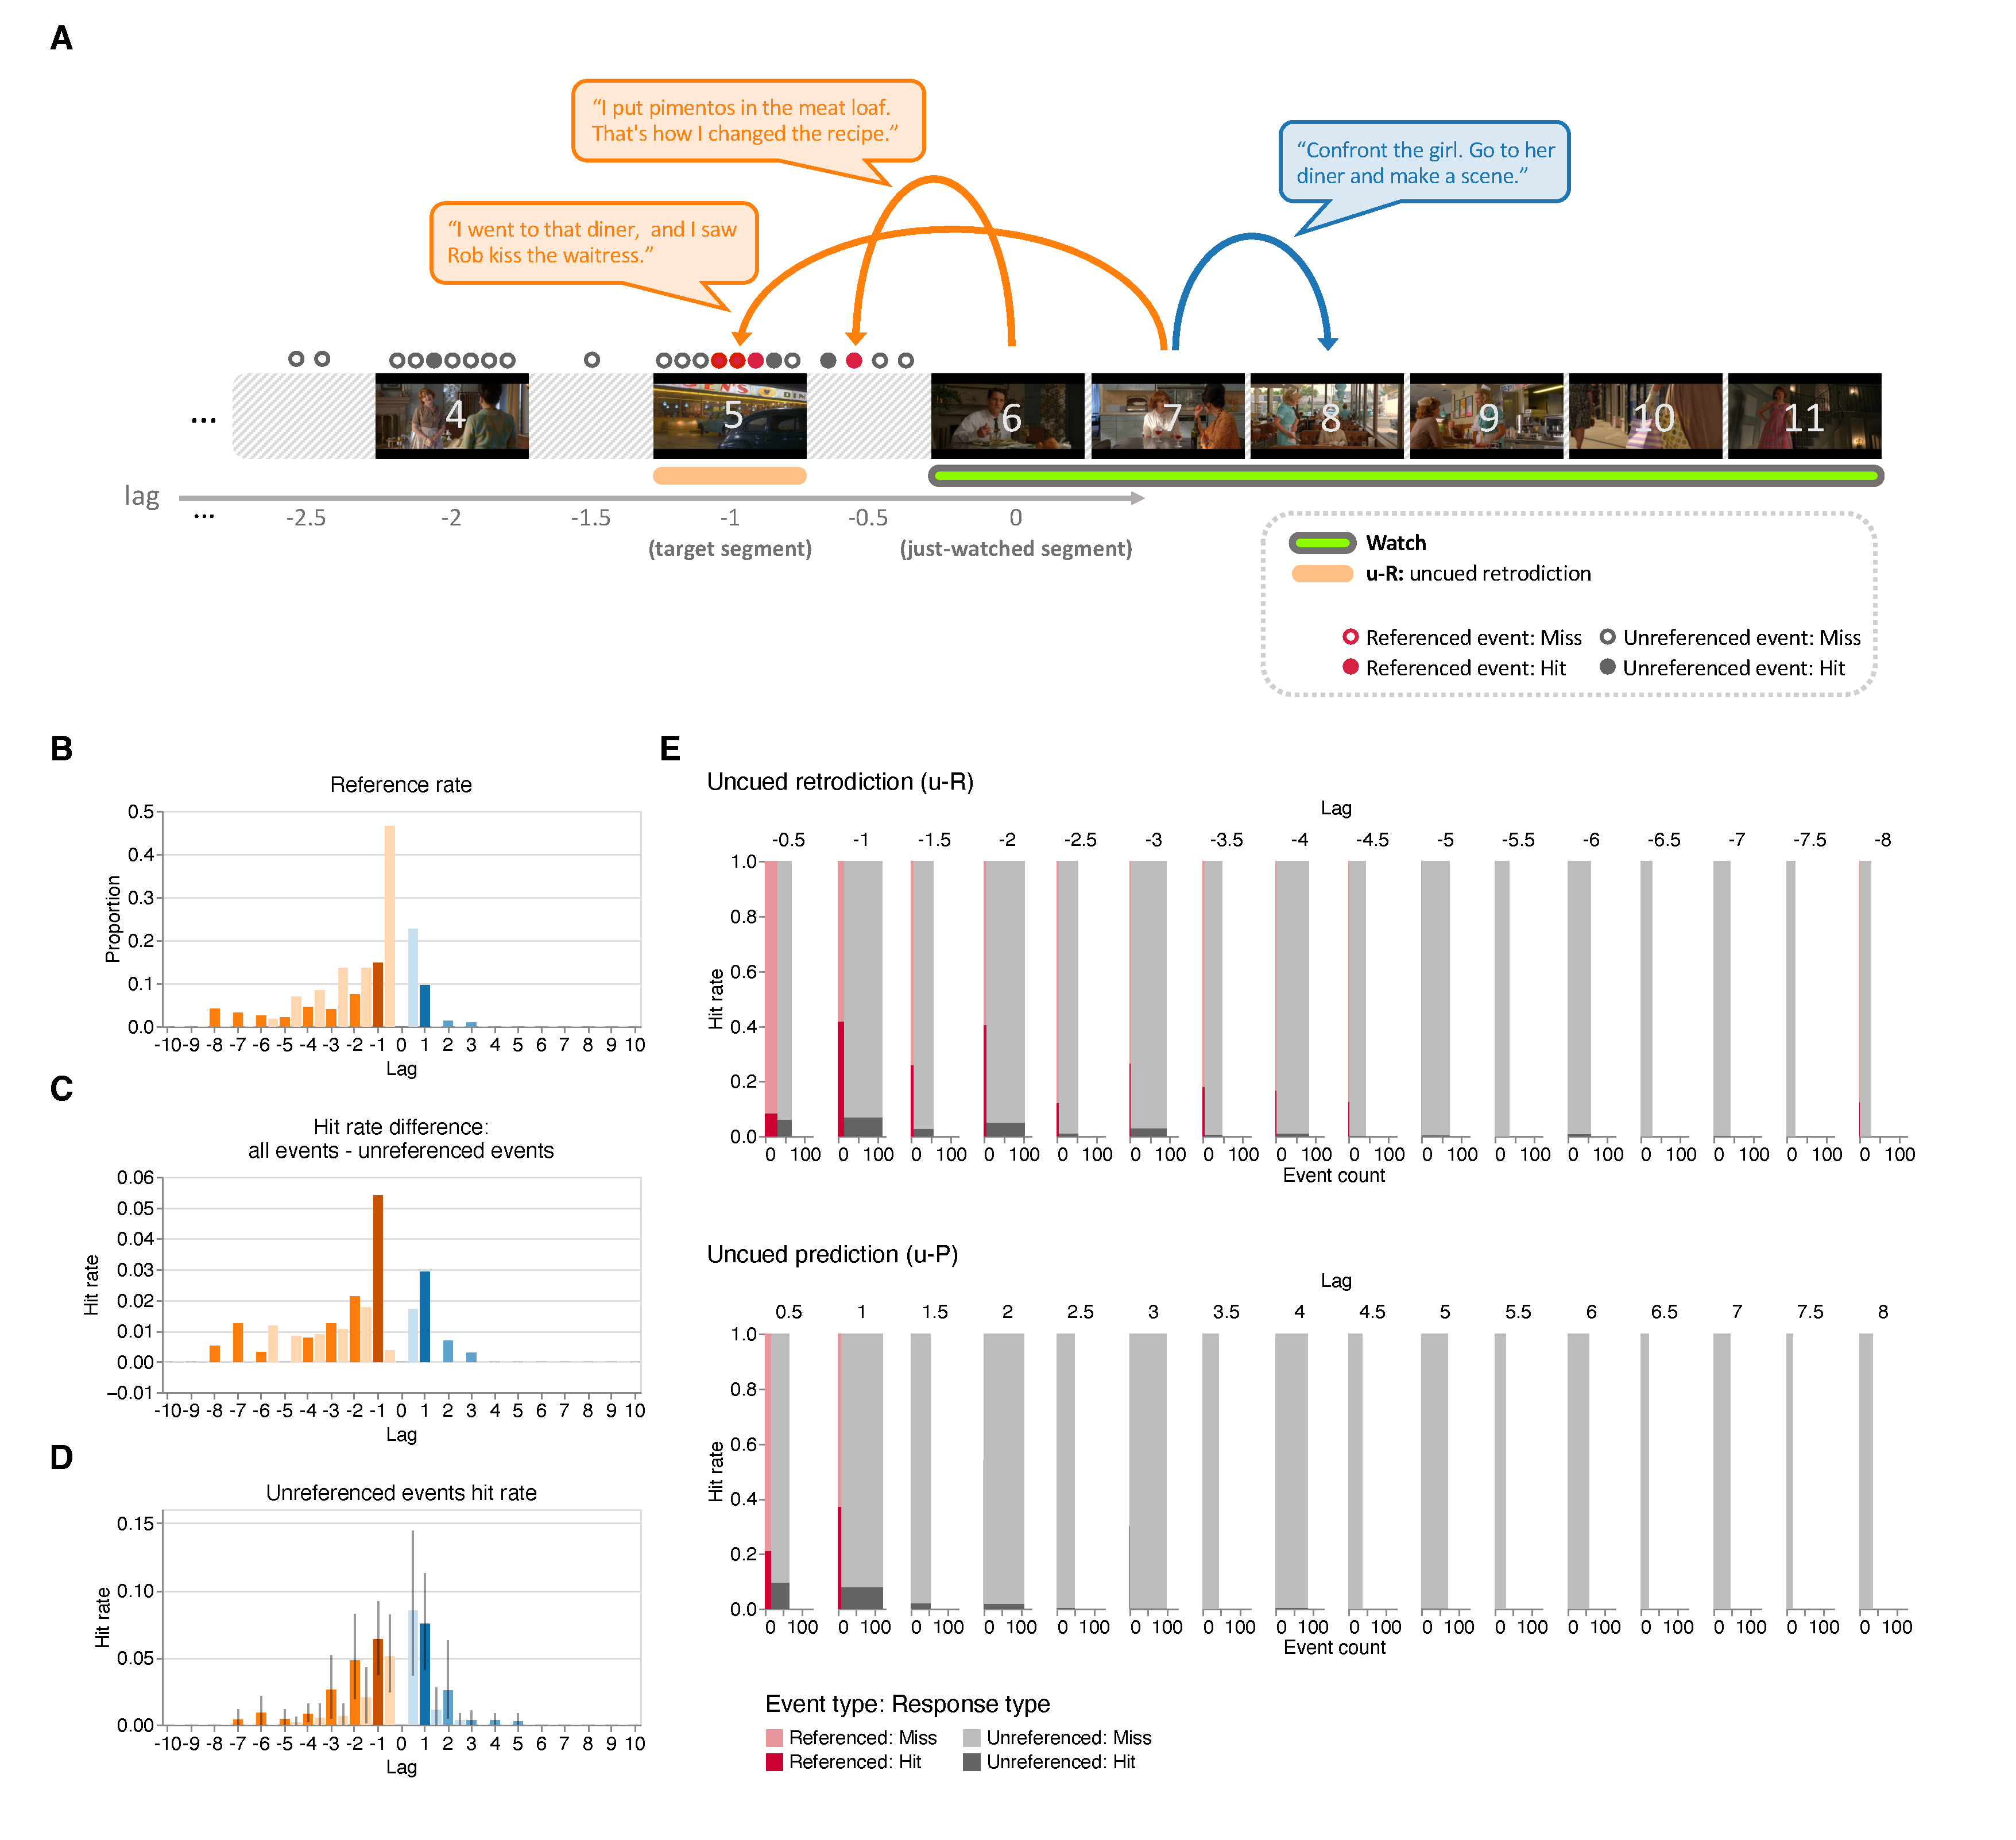
\includegraphics[width=0.9\textwidth]{results3}
%DIFDELCMD <   %%%
%DIFDELCMD < \caption{%
{%DIFAUXCMD
\textbf{\DIFdelFL{Characters' references drive participants' retrodiction and prediction performance.}}  %DIFAUXCMD
\textbf{\DIFdelFL{A. Illustration of annotation approach.}}  %DIFAUXCMD
\DIFdelFL{We manually annotated references to events in past or future segments in characters' spoken conversations.  We matched each such reference with its corresponding storyline event (and its corresponding segment number for onscreen events, or half-step segment number for offscreen events).  We then tracked the hit rate separately for referenced versus unreferenced events, in participants' uncued retrodictions and predictions.  }\textbf{\DIFdelFL{B. Reference rate as a function of lag.}}  %DIFAUXCMD
\DIFdelFL{Across all possible just-watched segments (lag 0), the bar heights denote the average proportions of events referenced in other past (orange, negative lags) or future (blue, positive lags) segments.  }\textbf{\DIFdelFL{C. Difference in hit rates between all events and unreferenced events.}}  %DIFAUXCMD
\DIFdelFL{To highlight the effect of characters' references to past and future events on participants' retrodictions and predictions, here we display the difference in across-segment mean hit rates between all events and unreferenced events, as a function of temporal distance (lag) to the just-watched segment.  }\textbf{\DIFdelFL{D. Hit rates for unreferenced events.}}  %DIFAUXCMD
\DIFdelFL{The average response hit rates for unreferenced events are displayed as a function of temporal distance to the just-watched segment.  Error bars denote bootstrapped 95\% confidence intervals.  Panels B--D: colors are described in the Figure~\ref{fig:result2} caption.  }\textbf{\DIFdelFL{E.  Hit rates and counts of referenced and unreferenced events.}}  %DIFAUXCMD
\DIFdelFL{As a function of temporal distance to the just-watched segment, the sub-panels display the across-segment mean numbers ($x$-axes) and hit rates ($y$-axes) of referenced (red) and unreferenced (gray) events that participants hit (darker shading) or missed (lighter shading) in their uncued retrodictions (top sub-panel) and uncued predictions (bottom sub-panel).}}
  %DIFAUXCMD
%DIFDELCMD < \label{fig:result3}
%DIFDELCMD < \end{figure}
%DIFDELCMD < 

%DIFDELCMD < %%%
\DIFdelend What might be driving participants to retrodict further and more accurately into the unobserved past, compared with their predictions of the unobserved future? By inspecting the video content, we noticed that characters \DIFdelbegin \DIFdel{in the television show }\DIFdelend frequently referenced both past events and (planned or predicted) future events in their spoken conversations\DIFaddbegin \DIFadd{, which might provide clues about past and future events}\DIFaddend . We wondered whether \DIFdelbegin \DIFdel{the characters' references might show temporal asymmetries that might explain participants' behaviors}\DIFdelend \DIFaddbegin \DIFadd{participants' responses might be influenced by characters' conversational references}\DIFaddend . Across all of the characters' conversations, and across all of the video segments \DIFaddbegin \DIFadd{from our main experiment}\DIFaddend , we manually identified a total of 82 references to past or future events (i.e., that occurred onscreen or offscreen before or after the events depicted in the current segment; \DIFdelbegin \DIFdel{Fig}\DIFdelend \DIFaddbegin \DIFadd{Figs}\DIFaddend .~\ref{fig:result3}A,\DIFdelbegin %DIFDELCMD < \references %%%
\DIFdel{A}\DIFdelend \DIFaddbegin \DIFadd{~\refer A, also see }\textit{\DIFadd{Reference coding}}\DIFaddend ). Characters \DIFaddbegin \DIFadd{in our main experiment's stimulus }\DIFaddend tended to reference the past (52 references) more than the future (30 references), consistent with previous work~\citep{DemiEtal18}. References to the past were also skewed to more temporally distant events compared with references to the future (Figs.~\ref{fig:result3}B,~\DIFdelbegin %DIFDELCMD < \references %%%
\DIFdelend \DIFaddbegin \DIFadd{\refer }\DIFaddend B). These \DIFaddbegin \DIFadd{asymmetries also held for characters in the replication experiment's stimulus (46 past references versus 7 future references, Figs.~\refEffectRep A,~\referRep B). These }\DIFaddend observations indicate that the characters in the \DIFdelbegin \DIFdel{stimulus display a preference }\DIFdelend \DIFaddbegin \DIFadd{stimuli display a ``preference'' }\DIFaddend for the past (versus future) in their conversations. Might this asymmetry be driving the asymmetries in participants' retrodictions versus predictions?


\DIFaddbegin \begin{figure}[tp]
  \centering
  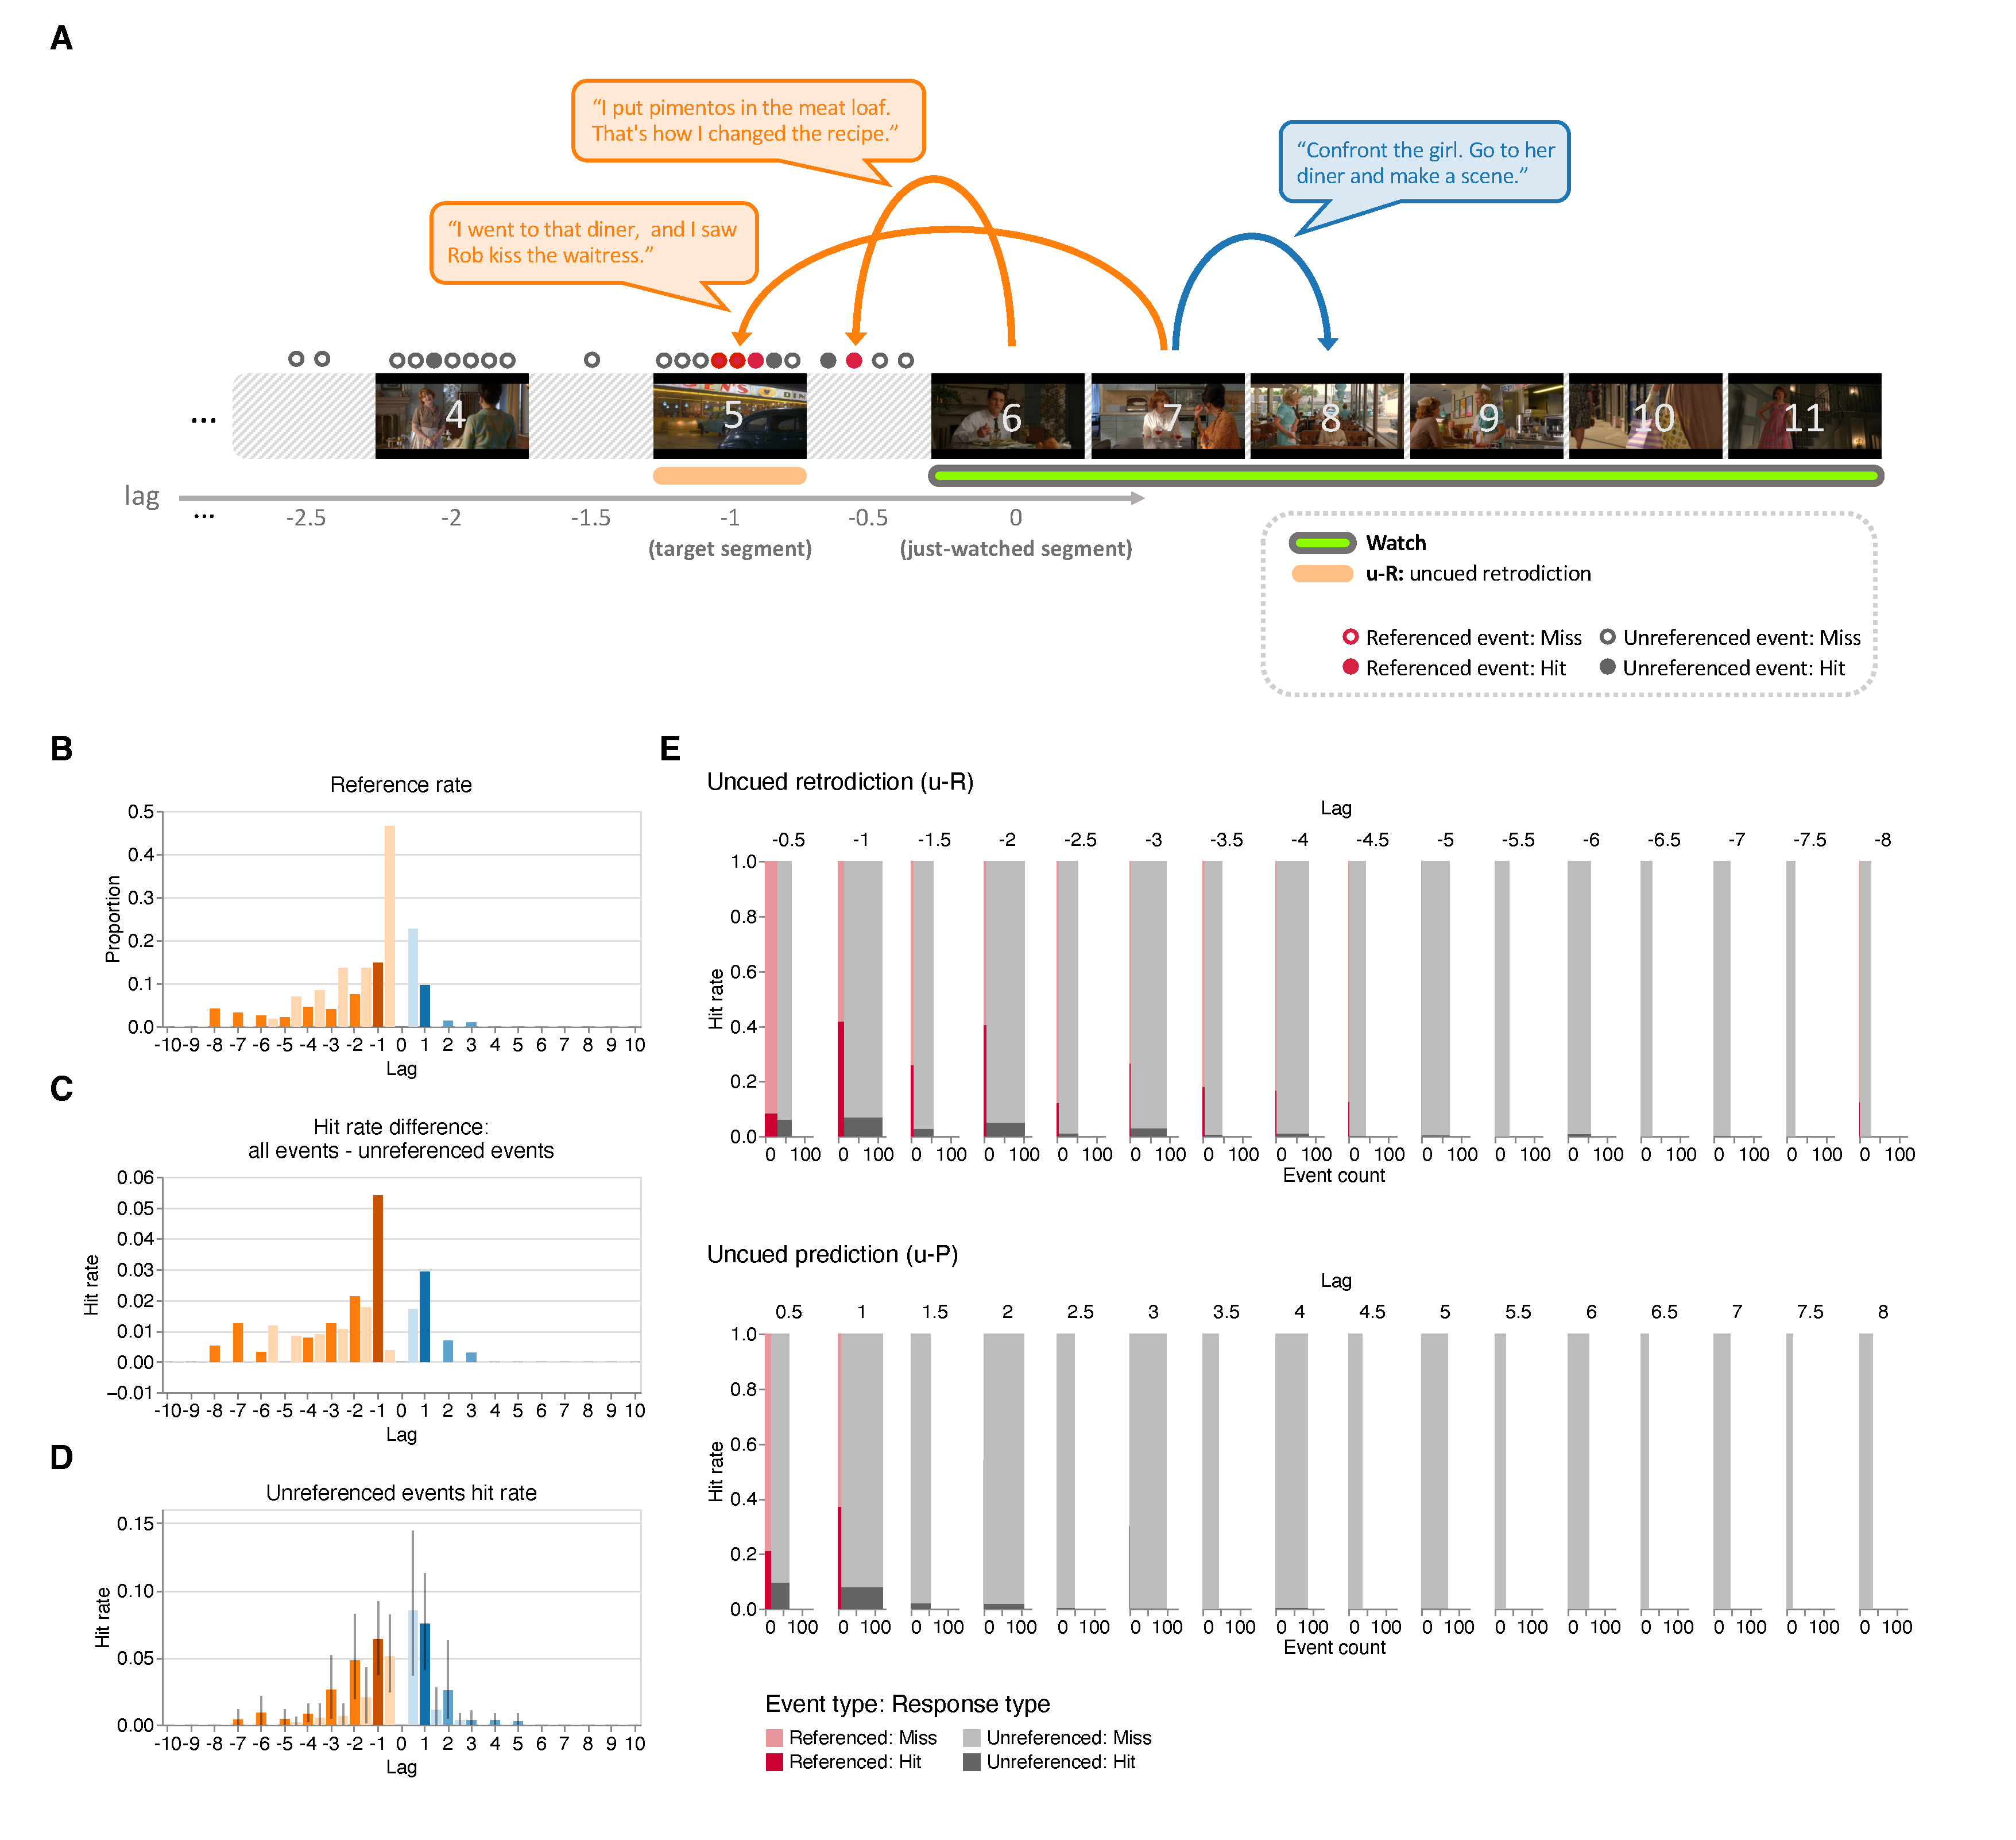
\includegraphics[width=0.8\textwidth]{results3}

  \caption{\textbf{\DIFaddFL{Characters' references drive participants' retrodiction and prediction performance (main experiment).}} \textbf{\DIFaddFL{A. Illustration of annotation approach.}} \DIFaddFL{We manually annotated references to events in past or future segments in characters' spoken conversations. We matched each such reference with its corresponding storyline event (and its corresponding segment number for onscreen events, or half-step segment number for offscreen events). We then tracked the hit rate separately for referenced versus unreferenced events in participants' uncued retrodictions and predictions. }\textbf{\DIFaddFL{B. Reference rate as a function of lag.}} \DIFaddFL{Across all possible just-watched segments (lag 0), the bar heights denote the average proportions of events referenced in other past or future segments. }\textbf{\DIFaddFL{C. Difference in hit rates between all events and unreferenced events.}} \DIFaddFL{To highlight the effect of characters' references to past and future events on participants' retrodictions and predictions, here we display the difference in across-segment mean hit rates between all events and unreferenced events, as a function of temporal distance (lag) to the just-watched segment. }\textbf{\DIFaddFL{D. Hit rates for unreferenced events.}} \DIFaddFL{The average response hit rates for unreferenced events are displayed as a function of temporal distance to the just-watched segment. Error bars denote bootstrapped 95\% confidence intervals. Panels B--D: colors are described in the Figure~\ref{fig:result2} caption. }\textbf{\DIFaddFL{E. Hit rates and counts of referenced and unreferenced events.}} \DIFaddFL{As a function of temporal distance to the just-watched segment, the sub-panels display the across-segment mean numbers ($x$-axes) and hit rates ($y$-axes) of referenced (red) and unreferenced (gray) events that participants hit (darker shading) or missed (lighter shading) in their uncued retrodictions (top sub-panel) and uncued predictions (bottom sub-panel). Intuitively, the widths of the rectangles at each lag denote the total number of events at each possible lag. The darker shading denotes the proportions of events that participants retrodicted or predicted, and the lighter shading denotes the proportions of events that participants ``missed'' in their responses. For an analogous presentation of results from the replication experiment, see Figure~\refEffectRep.}}

  \label{fig:result3}
\end{figure}

\DIFaddend Controlling for temporal distance (lag), past and future events that story characters referenced in their conversations were associated with higher hit rates than unreferenced events \DIFaddbegin \DIFadd{in our main experiment }\DIFaddend (uncued retrodiction: OR = 12.70, $Z = 10.94$, $p < 0.001$, CI: 8.06 to 20.03; uncued prediction: OR = 8.29, $Z = 6.83$, $p < 0.001$, CI: 4.52 to 15.20; Fig.~\ref{fig:result3}E). \DIFdelbegin \DIFdel{This indicates that }\DIFdelend \DIFaddbegin \DIFadd{In our replication study this result held for past events (uncued retrodiction: OR = 5.57, $Z = 5.88$, $p < 0.001$, CI: 3.14 to 9.89) but not for future events (uncued prediction: OR = 1.54, $Z = 0.22$, $p = 0.83$, CI: 0.03 to 73.36; Fig.~\refEffectRep D). The failure to replicate the ``prediction'' result appeared to follow from the fact that references to future events in characters' conversations were very rare in our replication experiment's stimulus.  These findings suggest that }\DIFaddend participants' responses are at least partially influenced by the characters' conversations. To estimate the contributions of characters’ references on hit rates, we computed the difference in hit rates between all events (which comprised both referenced and unreferenced events) and unreferenced events, as a function of lag. These differences exhibited a temporal asymmetry in favor of retrodiction (\DIFdelbegin \DIFdel{Fig}\DIFdelend \DIFaddbegin \DIFadd{Figs}\DIFaddend .~\ref{fig:result3}C\DIFaddbegin \DIFadd{,~\refEffectRep B}\DIFaddend ). This indicates that the asymmetries in participants' retrodictions versus predictions are also at least partially influenced by the characters' conversations. However, these temporal asymmetries in participants' retrodictions and predictions persisted even for events that characters never referenced in their conversations \DIFaddbegin \DIFadd{in both our main experiment }\DIFaddend (hit rates of uncued retrodicted versus predicted unreferenced events: OR = 2.00, $Z = 2.40$, $p = 0.02$, CI: 1.14 to 3.51; Fig.~\ref{fig:result3}D) \DIFdelbegin \DIFdel{.  }\DIFdelend \DIFaddbegin \DIFadd{and replication experiment (OR = 3.67, $Z = 2.61$, $p = 0.01$, CI: 1.38 to 9.74; Fig.~\refEffectRep C). }\DIFaddend When we further separated the unreferenced events into onscreen events and offscreen events, we found that these asymmetries held only for the onscreen events \DIFaddbegin \DIFadd{in our main experiment }\DIFaddend (onscreen: OR = 2.65, $Z = 2.59$, $p = 0.01$, CI: 1.27 to 5.54; offscreen: OR = 1.50, $Z = 0.91$, $p = 0.36$, CI: 0.63 to 3.62)\DIFaddbegin \DIFadd{, and only for offscreen events in our replication experiment (onscreen: OR = 0.97, $Z = -0.06$, $p = 0.95$, CI: 0.37 to 2.57; offscreen: OR = 13.88, $Z = 3.06$, $p = 0.002$, CI: 2.58 to 7.48)}\DIFaddend . Taken together, these analyses suggest that asymmetries in the number of references characters make to past and future events partially (but not entirely) explain why participants tend to retrodict the past further and more accurately than they predict the future.

\begin{figure}[tp]
  \centering
  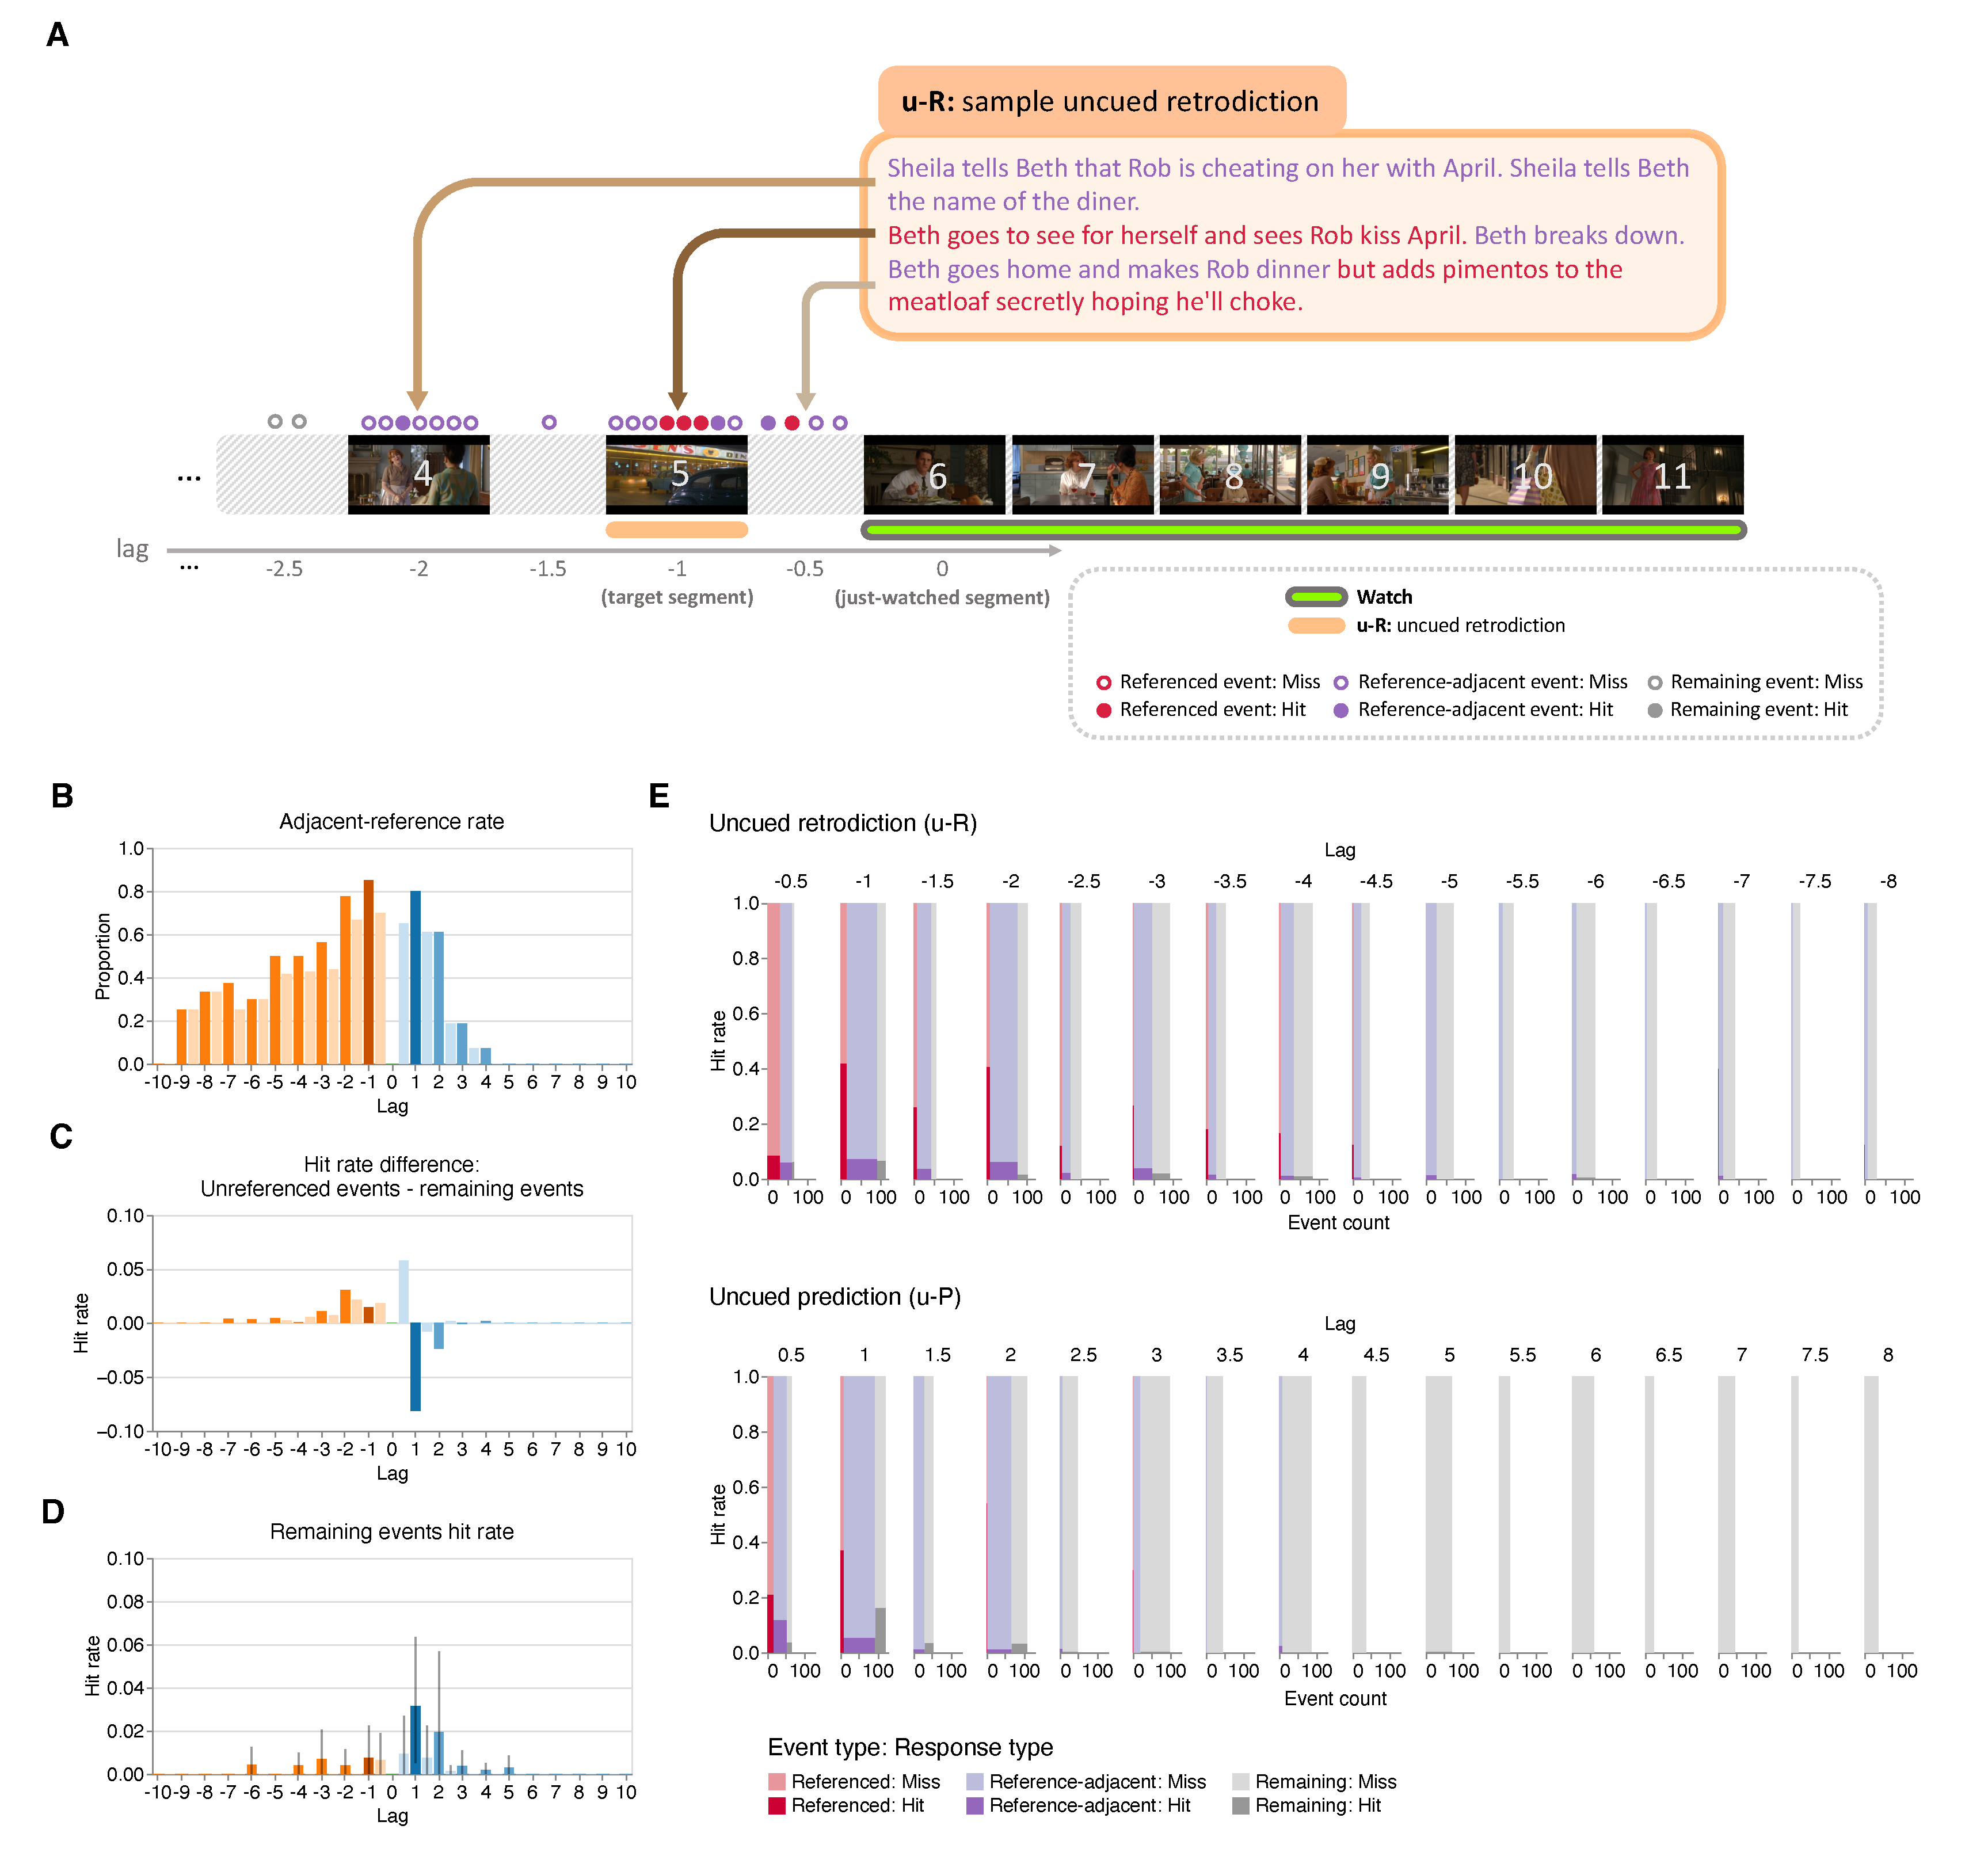
\includegraphics[width=0.8\textwidth]{results4}
\DIFaddbeginFL 

  \DIFaddendFL \caption{\DIFdelbeginFL \textbf{\DIFdelFL{Reference-adjacent events are associated with higher hit rates.}}  %DIFAUXCMD
\DIFdelendFL \DIFaddbeginFL \textbf{\DIFaddFL{Reference-adjacent events are associated with higher hit rates (main experiment).}} \DIFaddendFL \textbf{A. Illustration of annotation approach.} We extended the annotation procedure depicted in Figure~\ref{fig:result3}A to also label unreferenced events that were either temporally adjacent to (i.e., immediately preceding or proceeding) a referenced event (reference-adjacent events) or not (remaining events). \textbf{B. Adjacent reference rate for unreferenced events as a function of lag.} Across all possible just-watched segments (lag 0), the bar heights denote the average proportion of unreferenced events in other past \DIFdelbeginFL \DIFdelFL{(orange, negative lags) }\DIFdelendFL or future \DIFdelbeginFL \DIFdelFL{(blue, positive lags) }\DIFdelendFL segments that were temporally adjacent to any referenced event. \textbf{C. Difference in hit rates between unreferenced events and remaining events.} To highlight the effect of reference adjacency on retrodiction and prediction of unreferenced events, here we display the difference in across-segment mean hit rates between unreferenced events and remaining events, as a function of temporal distance (lag) to the just-watched segment. \textbf{D. Hit rates for remaining events.} The across-segment mean response hit rates for unreferenced events that were \textit{not} temporally adjacent to any referenced events are displayed as a function of temporal distance to the just-watched segment. Error bars denote bootstrapped 95\% confidence intervals. Panels B--D: colors are described in the Figure~\ref{fig:result2} caption. \textbf{E. Hit rates and counts of referenced, reference-adjacent, and remaining events.} As a function of temporal distance to the just-watched segment, the sub-panels display the numbers ($x$-axes) and proportions ($y$-axes) of referenced (red), reference-adjacent (purple), and remaining (gray) events that participants hit (darker shading) or missed (lighter shading) in their uncued retrodictions (top sub-panel) and uncued predictions (bottom sub-panel). \DIFaddbeginFL \DIFaddFL{For an analogous depiction of results from our replication experiment see Figs.~\refAdjacent~and~\refAdjacentCorrected.}\DIFaddendFL }
\DIFaddbeginFL 

  \DIFaddendFL \label{fig:result4}
\end{figure}

If characters' direct references cannot fully account for the temporal asymmetry in retrodicting the unobserved past versus predicting the unobserved future, what other factors might explain this phenomenon? The results above indicate that characters’ references to specific unobserved events in the past or future boost participants’ estimates of these events. \DIFaddbegin \DIFadd{But might characters' references have other effects on participants' responses }\textit{\DIFadd{beyond}} \DIFadd{the referenced events? For example, real-world experiences and events in realistic narratives are often characterized by temporal autocorrelations (i.e., what is ``happening now'' will likely relate to what happens ``a moment from now,'' and so on). Real-world experiences and realistic narratives are also often structured into ``schemas'' whereby experiences unfold according to a predictable pattern or formula that characterizes a particular situation, such as going to a restaurant or catching a flight at the airport~\mbox{%DIFAUXCMD
\citep{BaldEtal18}}\hskip0pt%DIFAUXCMD
. }\DIFaddend If there are associations \DIFdelbegin \DIFdel{and }\DIFdelend \DIFaddbegin \DIFadd{or temporal }\DIFaddend dependencies between temporally \DIFdelbegin \DIFdel{adjacent events , might characters’ references to specific events also boostparticipants’ estimates of other }\DIFdelend \DIFaddbegin \DIFadd{nearby events in the television shows participants watched, participants might be able to pick up on these patterns in forming their responses. This would be reflected in an inference ``boost'' for }\DIFaddend events that were \DIFdelbegin \DIFdel{temporally }\DIFdelend \textit{\DIFdelbegin \DIFdel{adjacent}\DIFdelend \DIFaddbegin \DIFadd{nearby in time}\DIFaddend } to \DIFaddbegin \DIFadd{events that characters referred to in their conversations, in addition to }\DIFaddend the referenced events \DIFaddbegin \DIFadd{themselves }\DIFaddend (Fig.~\ref{fig:result4}A)\DIFdelbegin \DIFdel{?  }\DIFdelend \DIFaddbegin \DIFadd{.
}

\DIFaddend Because characters tended to refer to past events more often than future events, the proportions of unreferenced events that were adjacent to referenced events should show a similar temporal asymmetry in favor of the past. We \DIFdelbegin \DIFdel{confirmed }\DIFdelend \DIFaddbegin \DIFadd{tested }\DIFaddend this intuition by computing the proportions of unreferenced events in the stimulus that were temporally adjacent to past or future events referenced by the characters during a given segment. Here we defined \textit{temporally adjacent} as any event within an absolute lag of one relative to a referenced onscreen event, or within an absolute lag of 0.5 to a referenced offscreen event. We also defined \textit{remaining} events as unreferenced events that were not temporally adjacent to any referenced events. \DIFdelbegin \DIFdel{As shown in Figure~\ref{fig:result4}B, }\DIFdelend \DIFaddbegin \DIFadd{In our main experiment }\DIFaddend we observed higher proportions of unreferenced past than future events that were temporally adjacent to referenced events \DIFdelbegin \DIFdel{.  }\DIFdelend \DIFaddbegin \DIFadd{(Fig.~\ref{fig:result4}B). }\DIFaddend Further, these reference-adjacent events had higher hit rates than remaining events after controlling for absolute lag (uncued retrodiction: OR = 7.15, $Z = 2.40$, $p = 0.02$, CI: 1.44 to 35.58; uncued prediction: OR = 3.11, $Z = 2.30$, $p = 0.02$, CI: 1.18 to 8.21; Fig.~\ref{fig:result4}E). To estimate the contributions of reference adjacency on hit rates, we computed the \DIFdelbegin \DIFdel{difference }\DIFdelend \DIFaddbegin \DIFadd{differences }\DIFaddend in hit rates between unreferenced events (which comprised both reference-adjacent and remaining events) and remaining events, as a function of lag. These differences exhibited a temporal asymmetry in favor of retrodiction \DIFdelbegin \DIFdel{.  }\DIFdelend \DIFaddbegin \DIFadd{(Fig.~\ref{fig:result4}C). }\DIFaddend This suggests that reference-adjacent events also contribute to participants' retrodiction advantage.  \DIFaddbegin \DIFadd{This reference-adjacency effect did not hold in our replication experiment (uncued retrodiction: OR = 6.46, $Z = 1.58$, $p = 0.13$, CI: 0.64 to 65.04; uncued prediction: OR = 0.002, $Z = 0.007$, $p = 0.99$, CI: $<0.001$ to $>9999$; Fig.~\refAdjacent D, B). Upon further examination of the stimulus we used in our replication experiment, along with participants' responses, we noticed that the television episode appears to comprise several interleaved storylines (Fig.~\refAdjacentCorrected A).  This meant that what we had originally labeled as ``reference-adjacent'' events (based solely on the temporal order in the }\textit{\DIFadd{episode}}\DIFadd{) did not necessarily correspond to chronological order in the }\textit{\DIFadd{story}}\DIFadd{.  For example, if (across successive segments) the narrative focuses on character $A$ at time $t$ in segment $n$, and on character $B$ at time $t$ in segment $n + 1$, then we reasoned that watching segment $n$ might not provide much insight into what would happen in segment $n + 1$.  However, watching segment $n$ }\textit{\DIFadd{could}} \DIFadd{provide clues about what would happen to character $A$ at time $t + 1$, which might have been shown later on in the episode.  When we ``corrected'' the reference-adjacency labels in the replication experiment stimulus to correspond to individual storylines, rather than solely with respect to the episode segment orders, we recovered the reference adjacent effect for uncued retrodiction (OR = 7.55, $Z = 2.93$, $p = 0.003$, CI: 1.95 to 29.20; Fig.~\refAdjacentCorrected E, C). We did not find a significant reference adjacent effect in uncued prediction (OR = 1176.66, $Z = 0.04$, $p = 0.97$, CI: $<0.001$ to $>9999$), again likely due to the limited number of future references in the narrative. }\DIFaddend Remaining events did \textit{not} exhibit a reliable temporal asymmetry (\DIFaddbegin \DIFadd{main experiment: }\DIFaddend OR = 0.75, $Z = 0.33$, $p = 0.74$, CI: 0.14 to 4.08; Fig.~\ref{fig:result4}D\DIFaddbegin \DIFadd{; replication experiment: OR = 889.48, $Z = 0.03$, $p = 0.97$, CI: $<0.001$ to $>9999$; Fig.~\refAdjacentCorrected D}\DIFaddend ), suggesting that, after accounting for temporal adjacency, character's references to past and future events can explain participants' retrodiction advantage.

\begin{figure}[tp]
  \centering
  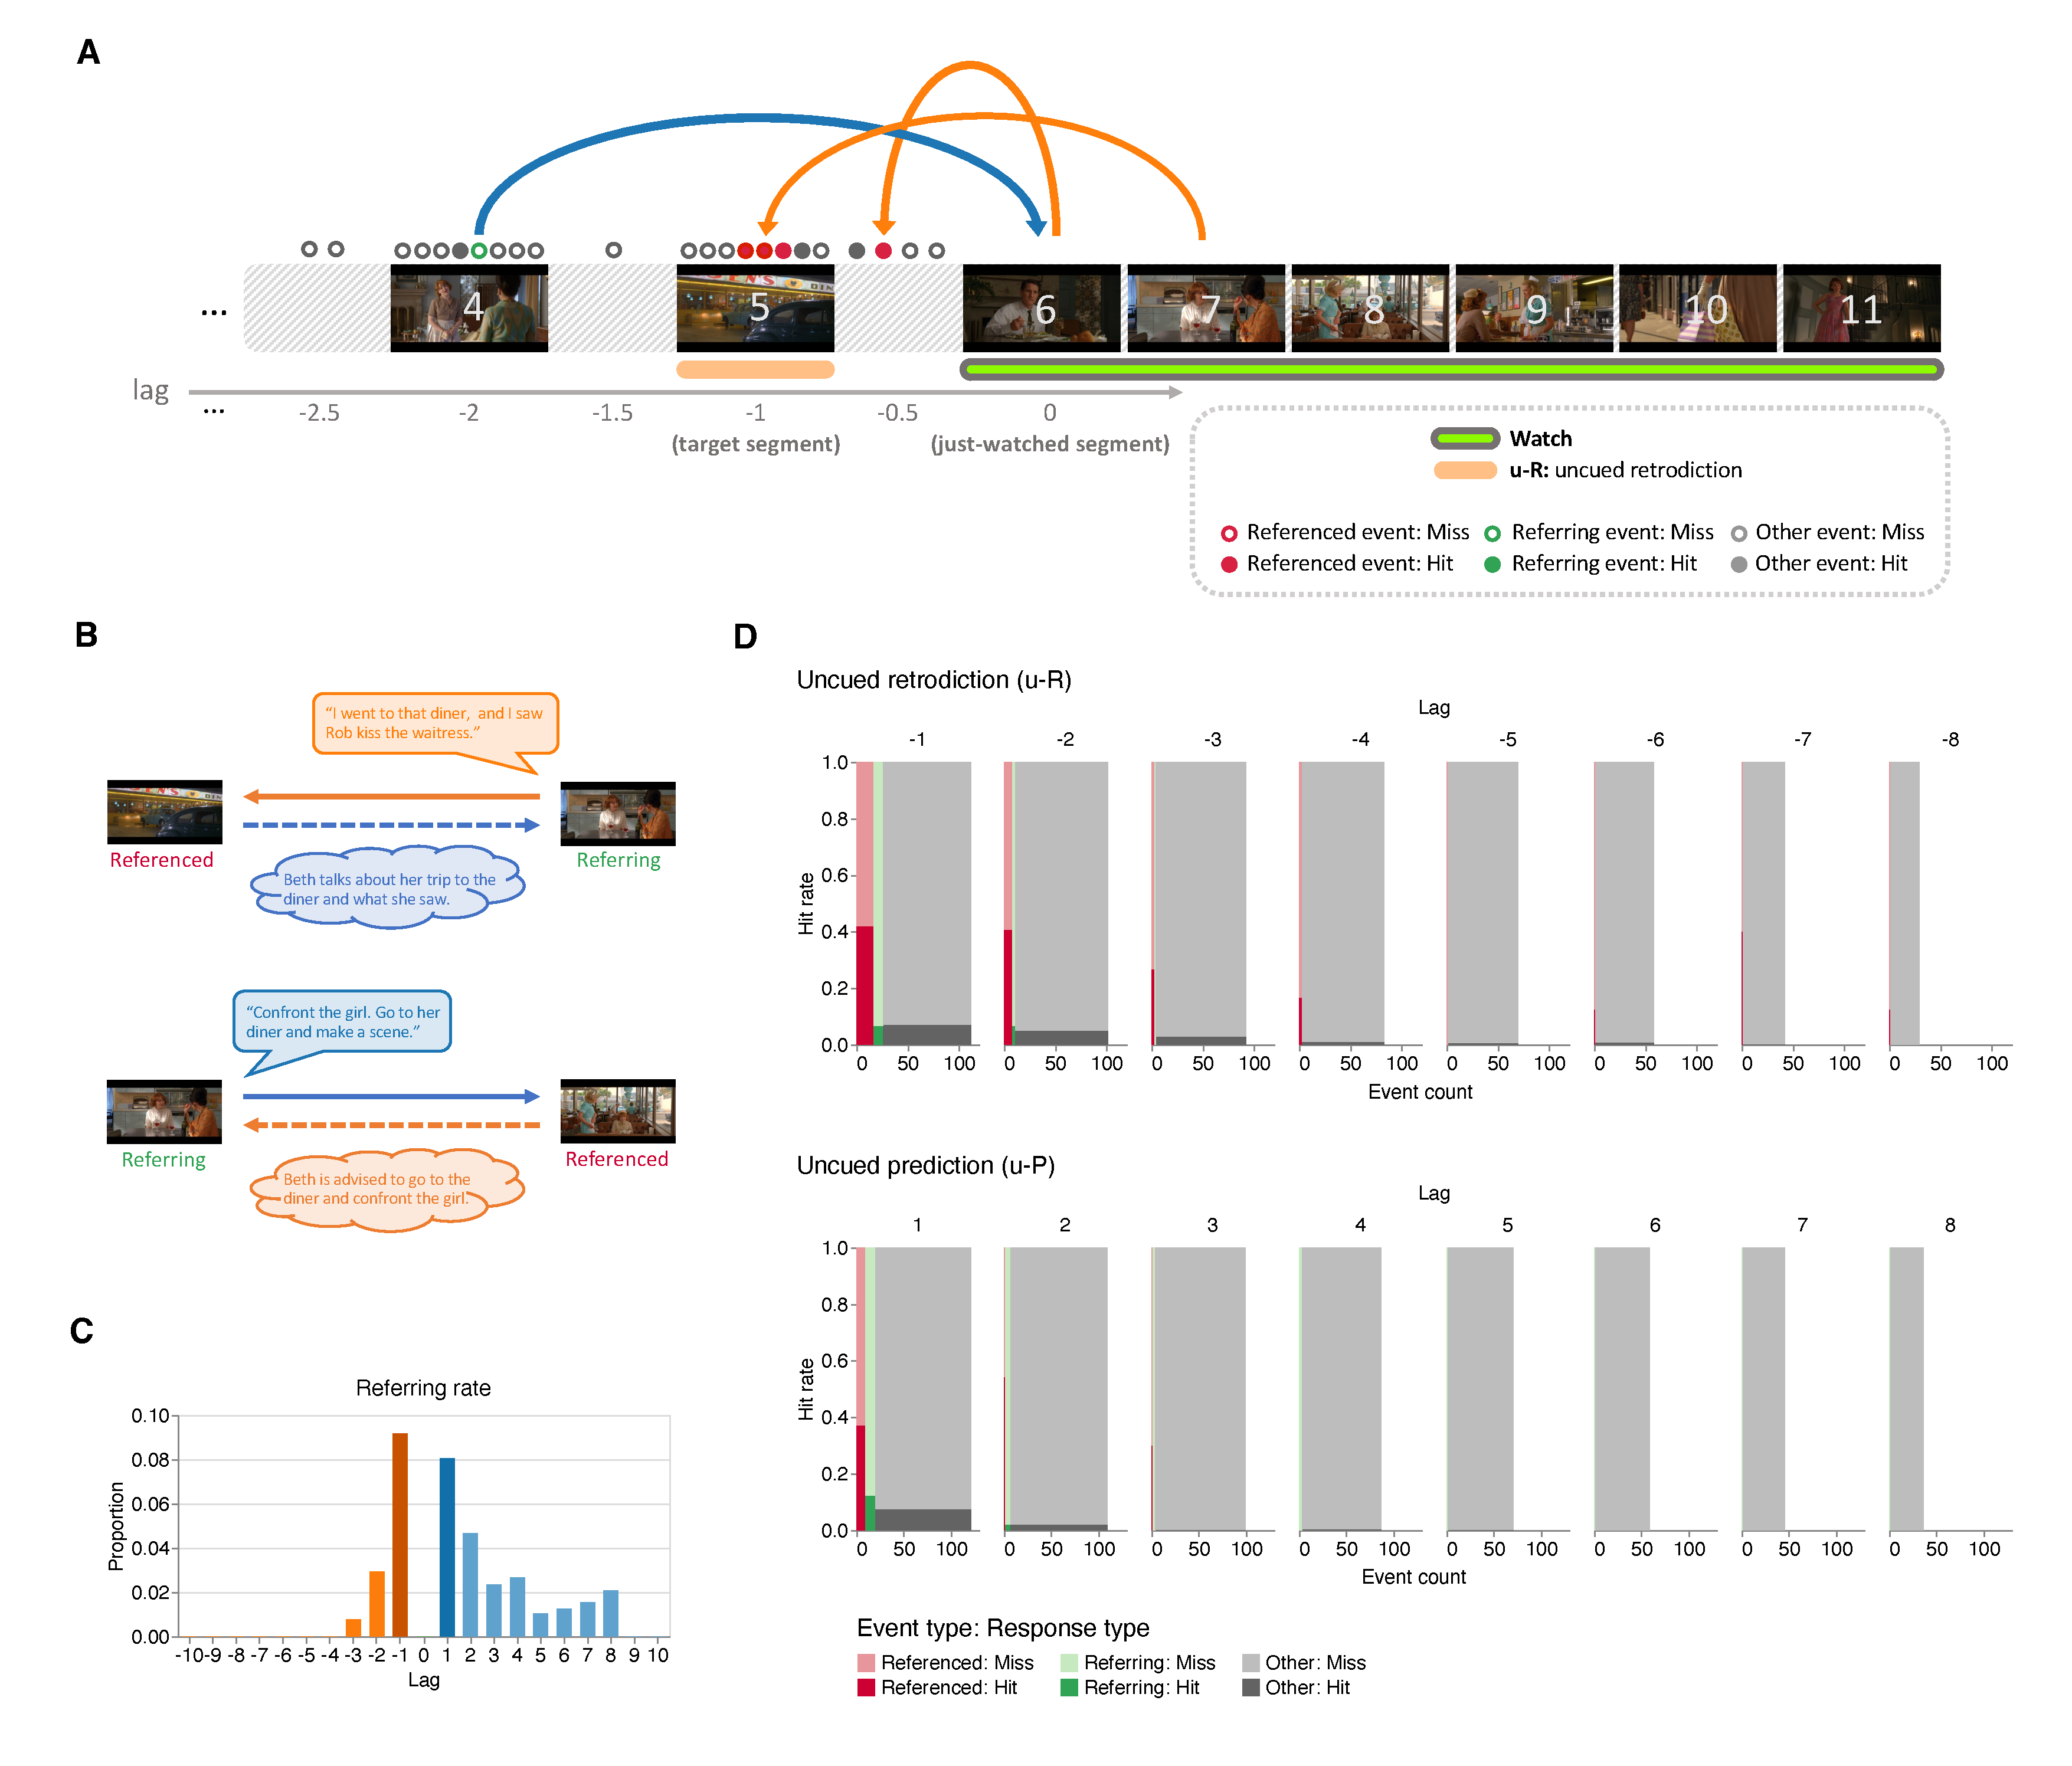
\includegraphics[width=\textwidth]{results5}
\DIFaddbeginFL 

  \DIFaddendFL \caption{\DIFdelbeginFL \textbf{\DIFdelFL{Referenced events are associated with higher hit rates, but referring events are not.}}  %DIFAUXCMD
\DIFdelendFL \DIFaddbeginFL \textbf{\DIFaddFL{Referenced events are associated with higher hit rates, but referring events are not (main experiment).}} \DIFaddendFL \textbf{A. Illustration of annotation approach.} We extended the annotation procedure depicted in Figure~\ref{fig:result3}A to also label which events \DIFaddbeginFL \DIFaddFL{in our main experiment's stimuli }\DIFaddendFL \textit{contained} references to events in other segments. \textbf{B. Referenced versus referring events.} During event $i$, when a character makes a reference to another event ($j$), we define $i$ as the \textit{referring} event and $j$ as the \textit{referenced} event. \textbf{C. Referring rate as a function of lag.} Across all possible just-watched segments (lag 0), the bar heights denote the across-segment mean proportions of events containing references to events in other past \DIFdelbeginFL \DIFdelFL{(orange, negative lags) }\DIFdelendFL or future \DIFdelbeginFL \DIFdelFL{(blue, positive lags) }\DIFdelendFL segments \DIFaddbeginFL \DIFaddFL{in our main experiment's stimuli}\DIFaddendFL . The bar colors are described in the Figure~\ref{fig:result2} caption. \textbf{D. Hit rates and counts of referenced, referring, and other events.} As a function of temporal distance to the just-watched segment, the sub-panels display the numbers ($x$-axes) and hit rates ($y$-axes) of referenced (red), referring (green), and other (gray) events that participants hit (darker shading) or missed (lighter shading) in their uncued retrodictions (top sub-panel) and uncued predictions (bottom sub-panel). \DIFaddbeginFL \DIFaddFL{For a display of analogous results from our replication experiment see Figure~\referringReferenced.}\DIFaddendFL }
\DIFaddbeginFL 

  \DIFaddendFL \label{fig:result5}
\end{figure}

The preceding analyses show that when characters reference past or future events, those referenced events, and other events that are temporally adjacent to the referenced events, are more likely to be retrodicted and predicted. In other words, referring to a past or future event in conversation leads to a ``boost'' in that event's hit rate. We wondered whether this boost was bi-directional. In particular: when a character refers (during a \textit{referring event}) to another event (i.e., the \textit{referenced event}), does this boost only the referenced event's hit rate, or does the referring event also receive a boost? We labeled each event as a ``referring event\DIFdelbegin \DIFdel{'',}\DIFdelend \DIFaddbegin \DIFadd{,'' }\DIFaddend a ``referenced event\DIFdelbegin \DIFdel{'',or a }\DIFdelend \DIFaddbegin \DIFadd{,'' or an }\DIFaddend ``other event'' (i.e., not referring or referenced; \DIFdelbegin \DIFdel{Fig}\DIFdelend \DIFaddbegin \DIFadd{Figs}\DIFaddend .~\ref{fig:result5}A, B). We limited our analysis to references to onscreen (explicit) events. Consistent with our analysis of \DIFdelbegin \DIFdel{character's references to other events (Fig}\DIFdelend \DIFaddbegin \DIFadd{the proportions of referenced events (Figs}\DIFaddend .~\ref{fig:result3}B\DIFdelbegin \DIFdel{), }\DIFdelend \DIFaddbegin \DIFadd{,~\refEffectRep A), the proportions of }\DIFaddend \textit{referring} events exhibited a \textit{forward} temporal asymmetry (Fig.~\ref{fig:result5}C\DIFaddbegin \DIFadd{,~\referringReferenced A}\DIFaddend ). Controlling for absolute lag, we found that referring events were associated with lower hit rates than referenced events \DIFaddbegin \DIFadd{in our main experiment }\DIFaddend (uncued retrodiction: OR = 0.03, $Z = -4.81$, $p < 0.001$, CI: 0.01 to 0.11; uncued prediction: OR = 0.04, $Z = -5.84$, $p < 0.001$, CI: 0.01 to 0.12; Fig.~\DIFdelbegin \DIFdel{\ref{fig:result3}}\DIFdelend \DIFaddbegin \DIFadd{\ref{fig:result5}}\DIFaddend D) and had no reliable differences in hit rates compared with other events (uncued retrodiction: OR = 0.37, $Z = -1.46$, $p = 0.15$, CI: 0.10 to 1.41; uncued prediction: OR = 2.16, $Z = 1.68$, $p = 0.09$, CI: 0.88 to 5.30). \DIFdelbegin \DIFdel{This }\DIFdelend \DIFaddbegin \DIFadd{In our replication experiment, because there were very few referenced events during prediction, which also resulted in limited referring events during retrodiction, we had insufficient data to reliably compare between referenced, referring, and other events (all $p$s $>0.99$; Fig.~\referringReferenced). Taken together, this }\DIFaddend indicates that only referenced events received a hit rate boost (relative to \DIFdelbegin \DIFdel{referring }\DIFdelend \DIFaddbegin \DIFadd{other }\DIFaddend events), suggesting that the retrodictive and predictive benefits of references are directed (i.e., asymmetric).


\DIFdelbegin \section*{\DIFdel{Discussion}}
%DIFAUXCMD
\DIFdel{We asked participants }\DIFdelend \DIFaddbegin \begin{figure}[tp]
  \centering
  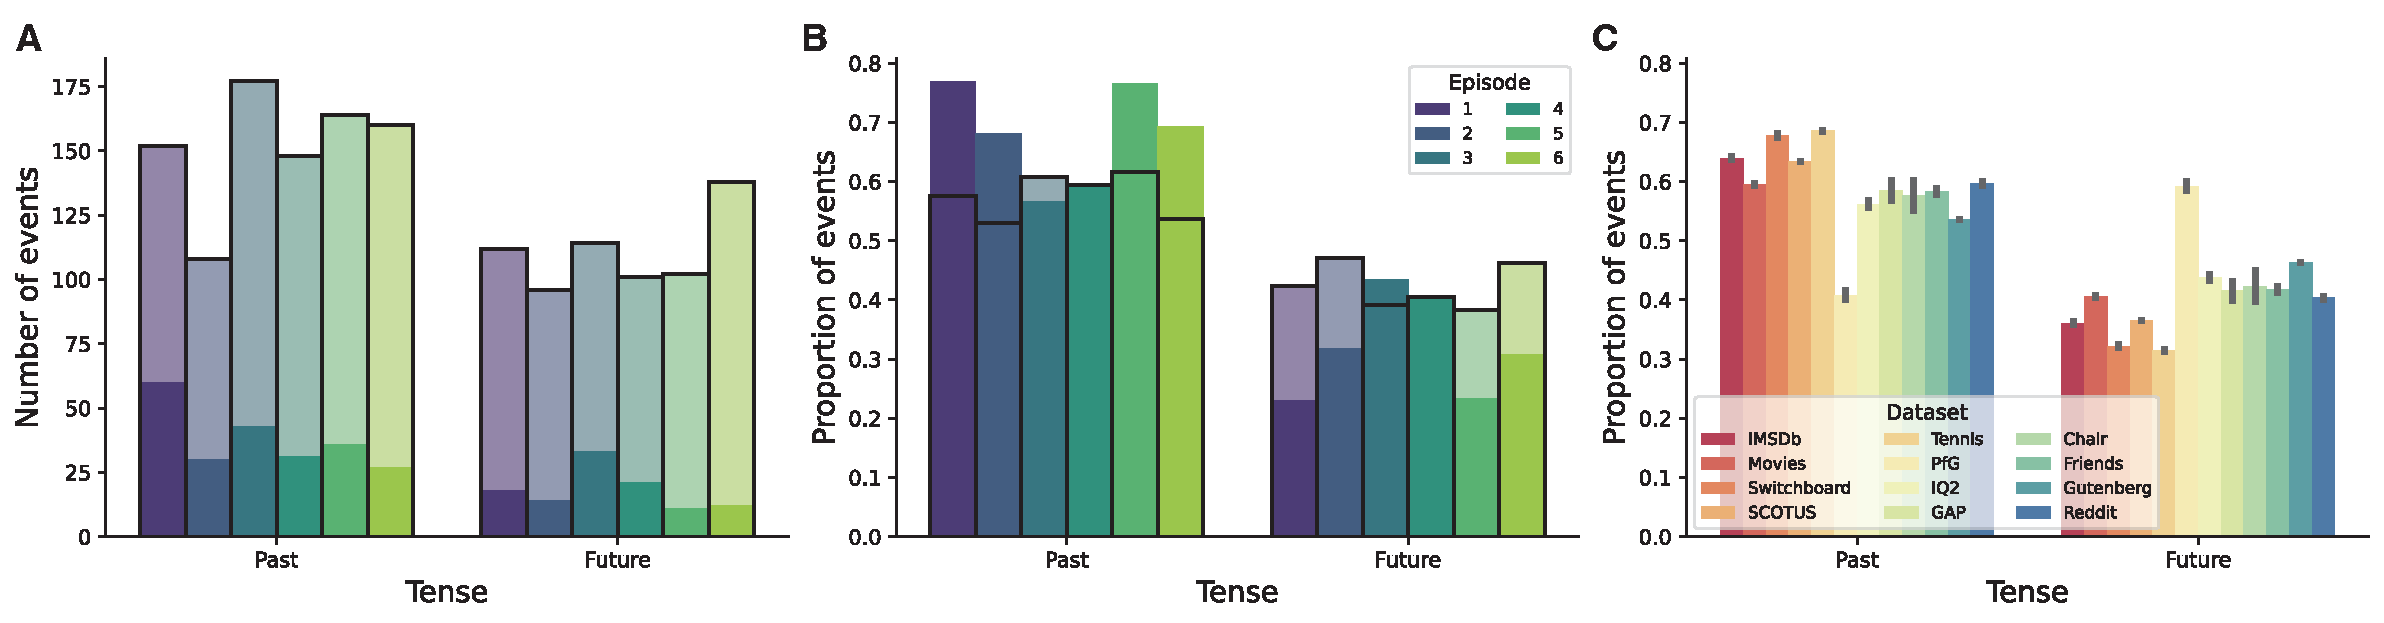
\includegraphics[width=\textwidth]{meta-analysis}

\caption{\textbf{\DIFaddFL{Meta analysis.}} \DIFaddFL{We used natural language processing to automatically identify references to past or future events across a variety of sources. }\textbf{\DIFaddFL{A. Numbers of past and future events in }\textit{\DIFaddFL{The Chair}}\DIFaddFL{, Season 1, Episodes 1--6.}} \DIFaddFL{The bar heights indicate the raw numbers of manually identified (lighter shading) and automatically identified (darker shading) past and future events from each episode (color). We used Episode 1 from this series as the stimulus in our replication experiment. }\textbf{\DIFaddFL{B. Proportions of past and future events in }\textit{\DIFaddFL{The Chair}}\DIFaddFL{, Season 1, Episodes 1--6.}} \DIFaddFL{The Panel is in the same format as Panel A, but here the bar heights have been divided by the total numbers of past and future events (per episode). }\textbf{\DIFaddFL{C. Proportions of past and future events in movies, television shows, and natural conversations.}} \DIFaddFL{As in Panel B, the bar heights denote the proportions of past and future events detected in each dataset (color). The datasets are described in Table~\metaAnalysisDatasets. Error bars denote bootstrap-estimated 95\% confidence intervals.}}

  \label{fig:meta-analysis}
\end{figure}

\DIFadd{The above analyses show that participants leveraged characters' references to make inferences about the past and the future, and the retrodiction advantage could be attributed to the fact that characters in the television shows we used as stimuli in our main experiment and replication experiment refer more often to the past than to the future. But how universal is this pattern? For example, were the television shows we happened to select for our experiment representative of television shows more generally? Or perhaps narratives created for entertainment purposes tend to have biases towards the past in order to keep the stories engaging and unpredictable. To better understand temporal biases in conversations, we carried out a meta analysis using extracted conversation data from several large datasets, comprising over 17 million documents. The data comprised transcripts from television shows and popular films, novels, and spoken and written utterances from natural conversations. A summary of the data we analyzed may be found in Table~\metaAnalysisDatasets. As summarized in Figure~\ref{fig:meta-analysis}, we used natural language processing to identify references to past or future events in each conversation (also see }\textit{\DIFadd{Meta analysis}}\DIFadd{).
}

\DIFadd{To validate our basic approach, we manually identified references to past and future events, across six episodes of the television show }\textit{\DIFadd{The Chair}} \DIFadd{(the first episode was used as the stimulus in our replication study). We then compared the numbers (Fig.~\ref{fig:meta-analysis}A) and proportions (Fig.~\ref{fig:meta-analysis}B) of automatically and manually identified references. In general, our automated tagging procedure tended to over-count the numbers of references. From manually ``spot checking'' hundreds of example tags, we noticed that our automated tagging procedure often counts the ``same'' references multiple times. Specifically, the manually generated tags sought to identify references to specific events that occurred or were implied to occur in other parts of the narrative. In contrast, as a heuristic, we designed the automated tagging procedure to identify uses of the past or future }\textit{\DIFadd{tense}} \DIFadd{as a proxy for references to past or future }\textit{\DIFadd{events}}\DIFadd{. Individual conversations often contains multiple references to a given (past or future) event. Whereas the manually generated tags counted these as ``single'' references, our automated tagging procedure had no means of differentiating between several references to the same event versus the same number of references to different events. This leads the automated tagging procedure to overestimate the numbers of distinct events being referenced. Nevertheless, this discrepancy did not appear to bias the balance of the overall }\textit{\DIFadd{proportions}} \DIFadd{of past or future references.
}

\DIFadd{In all, across all of the datasets we examined in our meta analysis, we identified a total of 36,008,500 references to past or future events. A total of 19,464,741 (54.06\%) of these were references to past events, and the remaining 16,543,759 (45.94\%) were references to future events. We also computed the average proportions of references to past and future events across documents within each individual dataset. Across the 12 datasets we examined (Fig.~\ref{fig:meta-analysis}, Tab.~\metaAnalysisDatasets), there were significantly more references to the past than the to the future (mean $\pm$ standard deviation proportion of references to past events: $58.99\% \pm 7.28\%$; $t(11) = 4.28, p = 0.0013$). We used the numbers of past references divided by the numbers of future references to quantify the effect size of temporal biases (see }\textit{\DIFadd{Meta analysis}}\DIFadd{).  Specifically, effect sizes greater than 1 reflect a bias towards the past, whereas effect sizes of less than 1 reflect a bias towards the future.  Across all 12 datasets, we observed an average effect size of 1.45 (standard error: 0.40); this indicates that references to the past are 1.45 times more prevalent than references to the future.  This bias towards the past also held for each dataset individually (range of effect sizes: 1.16 -- 2.18) except for one dataset, ``Persuasion for Good,'' which comprised natural conversations between pairs of Amazon Mechanical Turk workers wherein one participant tried to convince the other participant to donate to a charity in the future. In that dataset, references to the future were significantly more common than references to the past (effect size: $0.68 \pm 0.10$; CI: 0.59 }\DIFaddend to \DIFdelbegin \DIFdel{watch sequences of movie segments from a character-driven television drama. Across trials and participants, we controlled for how many segments preceding or proceeding the target segment the participants had seen, prior to watching the target segment.
Then we asked participants }\DIFdelend \DIFaddbegin \DIFadd{0.65). This latter example provided a nice sanity check for verifying that our general approach was not itself biased in favor of the past, e.g., even in conversations that were actually biased towards the future.  All of these effect sizes were significant at the $p < 0.001$ level or lower, except for the dataset containing transcripts of the six episodes of Season 1 of ``The Chair'' (average effect size: $1.50 \pm 0.20$; CI: 0.43 }\DIFaddend to \DIFdelbegin \DIFdel{either }\DIFdelend \DIFaddbegin \DIFadd{4.39; $p = 0.60$), which contained relatively few observations (therefore our confidence interval for that dataset was particularly large).  Taken together, the results from our meta analysis indicate that people tend to refer to the past more than they refer to the future, across a wide variety of situations (including in both fictional and real conversations). Although (as in the Persuasion for Good dataset) there may be specific exceptions to this bias, it seems that a bias in favor of the past is a common element of many (and perhaps even }\textit{\DIFadd{most}}\DIFadd{) human conversations.
}

\section*{\DIFadd{Discussion}}

\DIFadd{We asked participants in our main experiment to watch sequences of movie segments from a character-driven television drama and then either retrodict what had happened prior to a just-watched segment, }\DIFaddend predict what would happen next, \DIFdelbegin \DIFdel{retrodict what had happened before, or recount what had happened in the just-watched target segment}\DIFdelend \DIFaddbegin \DIFadd{or recall what they had just watched}\DIFaddend . We found that participants tended to more accurately and more readily retrodict the unobserved past than predict the unobserved future. We traced this temporal asymmetry to (a) characters\DIFdelbegin \DIFdel{’ }\DIFdelend \DIFaddbegin \DIFadd{' }\DIFaddend tendencies to refer to past events more than future events in their ongoing conversations, and (b) associations between temporally proximal events (Fig.~\ref{fig:discussion}). \DIFdelbegin \DIFdel{Our findings provide a number of important insights into how we make }\DIFdelend \DIFaddbegin \DIFadd{Essentially, associations between temporally proximal events serve to enhance asymmetries in inferences driven by conversational references (light orange and blue bars in Fig.~\ref{fig:discussion}). Our findings show that other peoples' psychological arrows of time can affect external observers' }\DIFaddend inferences about the unobserved past and future\DIFdelbegin \DIFdel{, and how we can study and quantify these processes. }\DIFdelend \DIFaddbegin \DIFadd{. We confirmed our main behavioral findings in a pre-registered replication study. We also carried out a meta analysis of tens of millions of utterances from television shows, movies, novels, and natural spoken and written conversations. We found that the tendency to refer more often to the past than the future appears to be a widespread characteristic of human conversation.
}\DIFaddend 

\begin{figure}[tp]
  \centering
  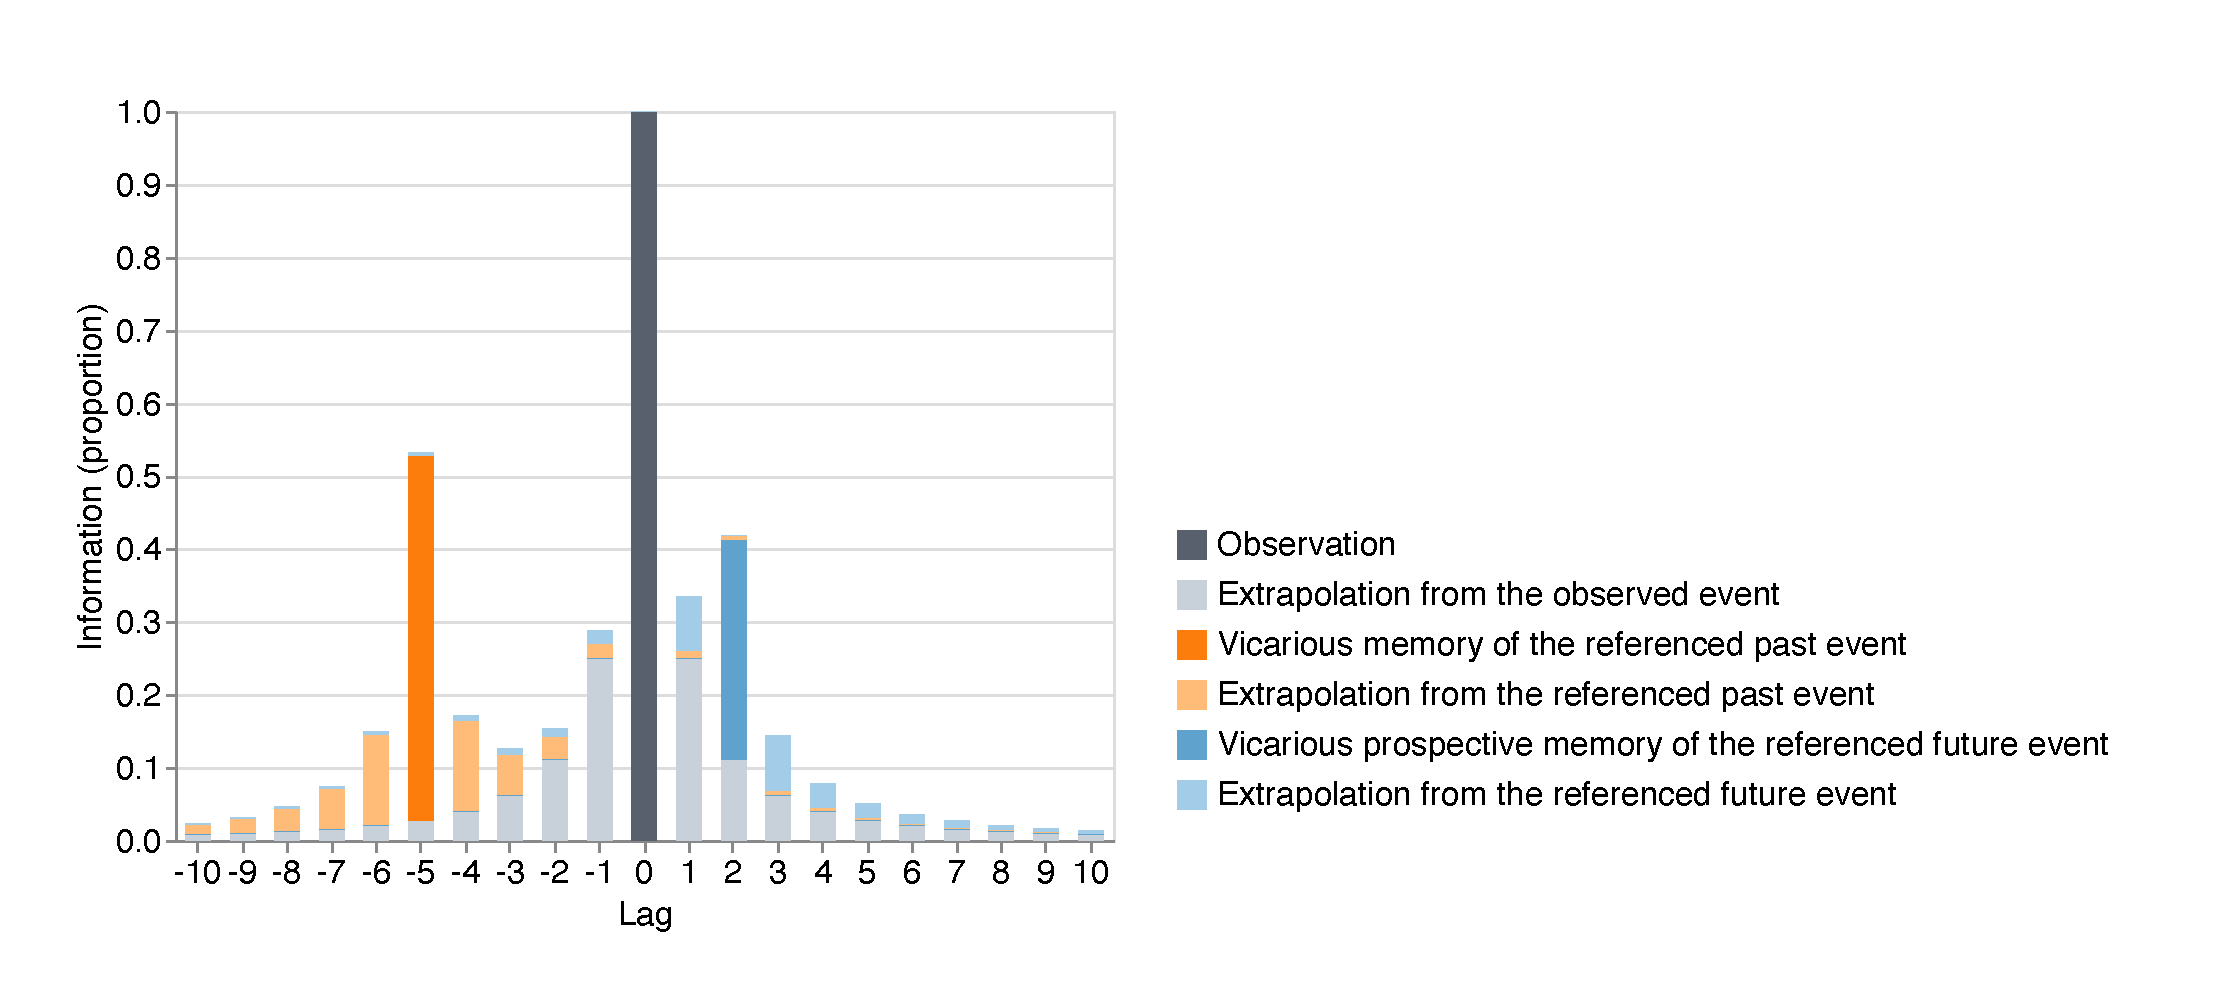
\includegraphics[width=\textwidth]{discussion}
\DIFaddbeginFL 

  \DIFaddendFL \caption{\DIFdelbeginFL \textbf{\DIFdelFL{How much information about the past and future can be extracted by observing the present?}}  %DIFAUXCMD
\DIFdelendFL \DIFaddbeginFL \textbf{\DIFaddFL{How much information about the past and future can be inferred by observing the present?}} \DIFaddendFL By definition, let us say that the present moment (lag 0) contains all information about itself (dark gray). Given learned statistical regularities, one might extrapolate from the present moment into the past or future (light gray). As illustrated in this schematic, the information contained in the present about other moments in time falls off with absolute lag. This falloff is approximately time-symmetric. References in the present to past events (dark orange) or future events (dark blue) provide additional information about those referenced moments in time, beyond what could be inferred solely from statistical regularities. This additional information about those referenced moments can also be extrapolated to other moments that are temporally nearby to \textit{them} (light orange and blue). \DIFaddbeginFL \DIFaddFL{The data in this schematic are hypothetical.}\DIFaddendFL }
\DIFaddbeginFL 

  \DIFaddendFL \label{fig:discussion}
\end{figure}

\DIFdelbegin \DIFdel{In free recall of random word lists, when the participant recalls the word studied at position $x$, they are likely to next recall the word studied at positions $x \pm 1$.  This phenomenon is termed the }\textit{\DIFdel{contiguity effect}}%DIFAUXCMD
\DIFdel{~\mbox{%DIFAUXCMD
\citep{Kaha96}}\hskip0pt%DIFAUXCMD
.  The contiguity effect has a well-characterized forward asymmetry~\mbox{%DIFAUXCMD
\citep{KahaEtal22}}\hskip0pt%DIFAUXCMD
, whereby the probability of next recalling the word from position $x + 1$ is more likely than recalling the word from position $x - 1$.  
This forward asymmetry suggests that we move through our memories with greater ease in the forward (versus reverse) temporal direction. Although our memory systems likely play a role in retrodiction and prediction~\mbox{%DIFAUXCMD
\citep{MomeHowa18, BarrEtal20, ChowEtal16}}\hskip0pt%DIFAUXCMD
, it is important to draw a distinction between our current paradigm and the circumstances leading to the forward asymmetry in the free recall contiguity effect. In free recall, for example, relative to the moment the word from position $x$ was studied, the response period is nearer in timeto the study of word $x + 1$ than to $x - 1$. In our paradigm, however, the past and future are equidistant from the present moment}\DIFdelend \DIFaddbegin \DIFadd{There exists a fundamental knowledge asymmetry such that we know more about our own past than the future, since we remember our past but not our future.  A number of prior studies have examined other temporal biases, such as how much people focus on the past, present, and future in their spontaneous thoughts~\mbox{%DIFAUXCMD
\citep{GranWals16, SongWang12, ShipAeon19}}\hskip0pt%DIFAUXCMD
, everyday conversations~\mbox{%DIFAUXCMD
\citep{DemiEtal18}}\hskip0pt%DIFAUXCMD
, and social media messages~\mbox{%DIFAUXCMD
\citep{ParkEtal17}}\hskip0pt%DIFAUXCMD
.  Several of these studies found that, on average, people's spontaneous }\textit{\DIFadd{internal}} \DIFadd{thoughts tend to be more future-oriented than past-oriented~\mbox{%DIFAUXCMD
\citep{GranWals16, SongWang12}}\hskip0pt%DIFAUXCMD
.  In contrast, people's external }\textit{\DIFadd{communications}} \DIFadd{tend to focus more on the past~\mbox{%DIFAUXCMD
\citep{ParkEtal17, DemiEtal18}}\hskip0pt%DIFAUXCMD
.  
}

\DIFadd{When people communicate through language or other observable behaviors, they can transmit their knowledge and memories to others~\mbox{%DIFAUXCMD
\citep{HirsEcht12, MahrCsib18, Dess07, ZadbEtal17}}\hskip0pt%DIFAUXCMD
. A consequence of this sharing across people is that biases or limitations in one person's knowledge and memories may also be transmitted to external observers. Although people }\textit{\DIFadd{can}} \DIFadd{communicate their intentions and future plans (i.e., information about their future), because people know }\textit{\DIFadd{more}} \DIFadd{about their pasts than their futures, the knowledge transmitted to observers is inherently biased in favor of the past~\mbox{%DIFAUXCMD
\citep[Fig.~\ref{fig:discussion}; ][]{DemiEtal18}}\hskip0pt%DIFAUXCMD
. Since observers leverage communicated knowledge to reconstruct the unobserved past and future, this explains why observers' inferences about observed people's lives also favor the past.
}

\DIFadd{People's knowledge asymmetries are not always directly observable. For example, in a conversation where someone talks exclusively about their future plans, a passive observer might gain more insight into the speaker's unobserved future than their unobserved past. However, because the speaker is also guided by their own psychological arrow of time, the ``upper limit'' of knowledge about their past is still higher than that of their future. Therefore, after accounting for knowledge that }\textit{\DIFadd{could}} \DIFadd{be revealed through active participation in the conversation, the seemingly future-biased conversation masks an underlying knowledge asymmetry in favor of the past. This hypothesized ``unmasking'' effect of interaction implies that the influence of other people's psychological arrows of time should be more robust when the receiver is an active participant in the conversation. Other social dimensions, such as trust, motivation or level of engagement, personal goals, and beliefs, might serve to modulate the effective ``gain'' of the communication channel-- i.e., how much the speaker's knowledge influences the observer's knowledge}\DIFaddend .

\DIFdelbegin \DIFdel{Several prior studies have examined retrodiction and prediction in statistical learning paradigms that use Markov sequences as stimuli.  In these paradigms, both infants~\mbox{%DIFAUXCMD
\citep{TummEtal16} }\hskip0pt%DIFAUXCMD
and adults~\mbox{%DIFAUXCMD
\citep{JonePash07}}\hskip0pt%DIFAUXCMD
show a (numerical) prediction advantage over retrodiction. During paired associates learning, when A–B pairs of items are presented simultaneously, participants generally show similar forward (generating B when cued with A) and backward (generating A when cued with B) performance~\mbox{%DIFAUXCMD
\citep{AschEben62, Kaha02}}\hskip0pt%DIFAUXCMD
. Taken together, these classic studies do not show the advantage for retrodiction over prediction that we observe here.  What accounts for these apparent discrepancies?  Why do people display a forward temporal asymmetry in free recall and for Markov sequences, temporal }\textit{\DIFdel{symmetry}} %DIFAUXCMD
\DIFdel{in paired associates learning, but a backward asymmetry in our task?  Our worksuggests that three main factors determine how readily participants infer one event from another in more complex }\DIFdelend \DIFaddbegin \DIFadd{In typical statistical sequences used in laboratory studies, there is no temporal asymmetry, either theoretically~\mbox{%DIFAUXCMD
\citep{Cove94, BialEtal01, ElliEtal09}}\hskip0pt%DIFAUXCMD
, or empirically~\mbox{%DIFAUXCMD
\citep{JonePash07}}\hskip0pt%DIFAUXCMD
. What makes narratives and real-world event sequences time-asymmetric? Of course there are many superficial differences between simple laboratory-manufactured sequences and real-world experiences. As one example, real-world experiences often involve other people who have their own memories and goals. Some recent work~\mbox{%DIFAUXCMD
\citep[e.g.,][]{TamiMitc13, MeyeEtal19b} }\hskip0pt%DIFAUXCMD
suggests that people might gain insights into other people using ``mental simulations'' of how they might respond in particular situations }\DIFaddend (e.g., \DIFdelbegin \DIFdel{``naturalistic’’) circumstances.  The first factor is that nearby events are associated.  This may follow from the notion that events in narratives, as in real-world experiences , tend to change gradually.  In other words, what is happening }\DIFdelend in \DIFaddbegin \DIFadd{the future), or of which sorts of prior experiences might have led someone to behave a particular way in }\DIFaddend the present\DIFdelbegin \DIFdel{moment (where you are located, what you are doing, who you are with, what you are thinking or feeling, etc. ) will, in general, be similar to what was happening a moment ago, and also to what will happen in the next moment. These similarities are roughly symmetric: the past and present are (on average) as similar as the present and future, after controlling for temporal distance. In our study, this symmetry provides a balanced forward }\textit{\DIFdel{and}} %DIFAUXCMD
\DIFdel{backward advantage for events that are nearby in time to the present moment (Fig. ~\ref{fig:discussion}, gray). The second factor is that, when characters in the narrative refer to other (temporally distant) moments, participants incorporate those references into their retrodictions and predictions (Fig. ~\ref{fig:result3}; dark orange and blue in Fig. ~\ref{fig:discussion}).
Other work has tended to focus on how memories can be shared across people through conversational references to }\textit{\DIFdel{prior}} %DIFAUXCMD
\DIFdel{experiences~\mbox{%DIFAUXCMD
\citep{HirsEcht12, MahrCsib18, Dess07}}\hskip0pt%DIFAUXCMD
.  Our study extends this notion by showing that ``memory sharing’’ need not be limited solely to past events. Rather, conversations can also provide information about the }\textit{\DIFdel{future}}%DIFAUXCMD
\DIFdel{, in the form of shared prospective memories .  Presumably due to inferred associations between temporally adjacent events , events that }\DIFdelend \DIFaddbegin \DIFadd{.  But at a higher level, }\DIFaddend are \DIFaddbegin \DIFadd{our subjective experiences essentially more complicated versions of laboratory-manufactured sequences? Or are there fundamental differences? One possibility is that real-life event sequences are not stationary~\mbox{%DIFAUXCMD
\citep[i.e., not in equilibrium; ][]{Cove94}}\hskip0pt%DIFAUXCMD
. For example, real-life events might start from a special initial condition~\mbox{%DIFAUXCMD
\citep{Albe00, Feyn65, Cove94} }\hskip0pt%DIFAUXCMD
and proceed through a series of transitions from more-ordered to less-ordered states, thus exhibiting an arrow time. When we retrodict, it is possible that we only consider possible past events that are compatible with the highly-ordered special initial state~\mbox{%DIFAUXCMD
\citep{Carr10, Carr16}}\hskip0pt%DIFAUXCMD
. For example, when we see a broken egg we might infer that the egg had been intact at some point in the past. But it would be difficult to guess at what states or forms the broken egg might take in the future~\mbox{%DIFAUXCMD
\citep{Carr10, Carr16}}\hskip0pt%DIFAUXCMD
. In other words, the procession from order to disorder might result in better retrodiction performance compared with that of (implicitly less-restricted) prediction tasks. The special initial state might also explain why we remember the past, but not the future. Some recent work suggests that the psychological arrow of time might be explained by a related concept in the statistical physics literature, termed the ``thermodynamic'' arrow of time~\mbox{%DIFAUXCMD
\citep{MlodBrun14, Rove22}}\hskip0pt%DIFAUXCMD
. However, the relation between the thermodynamic and psychological arrows of time is still under debate~\mbox{%DIFAUXCMD
\citep{Golo21, HemmShen19}}\hskip0pt%DIFAUXCMD
.
}

\DIFadd{Beyond forming inferences about unobserved past and future events, our work also relates to prior studies of how people perceive time~\mbox{%DIFAUXCMD
\citep{BlocGrub14, Howa18, Eagl08, IvrySchl08, Wear16}}\hskip0pt%DIFAUXCMD
, and how we ``move'' through time in our memories of our past experiences~\mbox{%DIFAUXCMD
\citep{Mann21a, MannEtal11, HowaEtal12, MannEtal07, ShanHowa12, Kaha96, PolyKaha08, SchaTulv94} }\hskip0pt%DIFAUXCMD
or in our imagined (past or future) experiences~\mbox{%DIFAUXCMD
\citep{Scha12, JossTone20, SchaEtal98, MomeHowa18}}\hskip0pt%DIFAUXCMD
. For example, a well-studied phenomenon in the episodic memory literature concerns how remembering a given event cues our memories of other events that we experienced }\DIFaddend nearby in time\DIFdelbegin \DIFdel{to a referenced eventalso receive a boost (Fig.~\ref{fig:result4}, light orange and blue in Fig.~\ref{fig:discussion}) .  We expect that these first two factors will hold across different narratives and real-world experiences, as associations between temporally proximal items and experiences have been widely documented~\mbox{%DIFAUXCMD
\citep[for review, see][]{KahaEtal22, Mann20}}\hskip0pt%DIFAUXCMD
. The third factor is that characters in the narrative used in our study tend to refer to past events more than future events (Fig. ~\ref{fig:result3}). This temporal asymmetry in the characters’ conversations is what }\DIFdelend \DIFaddbegin \DIFadd{~\mbox{%DIFAUXCMD
\citep[i.e., the \textit{contiguity effect};][]{Kaha96}}\hskip0pt%DIFAUXCMD
. Across a large number of studies there appears to be a nearly universal tendency for people to move }\textit{\DIFadd{forwards}} \DIFadd{in time in their memories, whereby recalling an ``event'' (e.g., a word on a previously studied list) is about twice as likely to be followed by recalling the event that immediately followed as compared with the event immediately preceding the just-recalled event~\mbox{%DIFAUXCMD
\citep{HealKaha14a}}\hskip0pt%DIFAUXCMD
. Superficially our current study }\DIFaddend appears to \DIFdelbegin \DIFdel{drive the advantage for retrodiction over prediction in our study. At least one prior study suggests that people are also more likely to refer to past (versus future) events in natural conversations~\mbox{%DIFAUXCMD
\citep{DemiEtal18}}\hskip0pt%DIFAUXCMD
. To the extent that this holds in general across narratives and experiences, we expect that the retrodiction advantage we observe here will apply in general.  However, we also hypothesize that in scenarios where people discuss the future }\textit{\DIFdel{more}} %DIFAUXCMD
\DIFdel{than the past, participants should show a }\textit{\DIFdel{prediction}} %DIFAUXCMD
\DIFdel{advantage.  Similarly, when the past and future are balanced in conversations, we hypothesize that the asymmetry should disappear.}\DIFdelend \DIFaddbegin \DIFadd{report the }\textit{\DIFadd{opposite}} \DIFadd{pattern, whereby participants display a }\textit{\DIFadd{backwards}} \DIFadd{temporal bias. However, the two sets of findings may be reconciled when one considers the frame of reference~\mbox{%DIFAUXCMD
\citep[and current mental context; e.g.,][]{HowaKaha02a} }\hskip0pt%DIFAUXCMD
of the participant at the moment they make their response. In our study, participants observe an event in the present, and they make guesses about what happened in the unobserved past or future, relative to the just-observed event. (Our findings imply that participants are more facile at moving backwards in time than forwards in time, relative to ``now.'') In contrast, the classic contiguity effect in episodic memory studies refers to how people move through time relative to a just }\textit{\DIFadd{remembered}} \DIFadd{event. The forward asymmetry in the contiguity effect follows from the notion that the moment of remembering has greater contextual overlap with events }\textit{\DIFadd{after}} \DIFadd{the remembered event from the past, including the moment of remembering, than events that happened before it~\mbox{%DIFAUXCMD
\citep[for review also see ][]{MannEtal15, Mann20}}\hskip0pt%DIFAUXCMD
.  In other words, our current frame of reference appears to exhibit a sort of ``pull'' on our thoughts, such that thoughts about recent experiences still lingering in our minds drag us towards the recent past, but after thinking about the more distant past we are dragged (relatively) forward in time back to ``now.''
}\DIFaddend 

%DIF <  Our memories give information about our past, but not our future.  Why do we only have memories of the past?  Why do we perceive time as flowing from the past \textit{to} the future?  The fundamental laws of physics are time-reversible: given the present position and velocity of a particle, the past and future states of that particle are equally knowable.  In the extreme, causal determinists have argued that an imaginary being who knew the positions and velocities of every particle in the universe (referred to as Laplace’s demon) would be able to perfectly compute the entire past and future states of the universe using classical mechanics~\citep{Hawk99}.  Given incomplete information, however, past and future are \textit{not} equal.  According to the second law of thermodynamics, the total entropy (e.g., uncertainty or randomness) in a system never decreases.  This ``thermodynamic arrow of time'' implies that the past will always be less uncertain than the future~\citep{Albe00, Carr10, Carr16}.  It is difficult to draw direct inferences about how the thermodynamic arrow of time might affect our memory systems.  One possibility is that the thermodynamic arrow of time may help to explain why we can remember the past but not the future~\citep{MlodBrun14, Rove22}, although this view is currently under debate~\citep{Golo21, HemmShen19}.  The thermodynamic arrow of time has two potential implications for our study.  First, to the extent that the thermodynamic arrow of time explains why we remember the past (but not the future), this gives people (and characters in realistic narratives) more information about their own pasts than about their own futures.  Second, the thermodynamic arrow of time also applies to the \textit{observers}' inferences about the past and future.  Because the past is inherently less uncertain than the future, this may confer an advantage to retrodiction over prediction.  A substantial challenge is that real-world events (unlike Markov processes) have no ground truth uncertainty.  Even attempts to \textit{estimate} uncertainty will be heavily dependent on which factors and scales we consider in our calculations.  When we group several microstates into the same macrostate~\citep[known as \textit{course-graining};][]{Rove14}, we make an implicit assumption about which ``level'' of granularity is relevant.  If we retrodict and predict with different degrees of course-graining, this will in turn affect the temporal symmetry of those processes.
\DIFdelbegin %DIFDELCMD < 

%DIFDELCMD < %%%
\DIFdelend In our study, we explicitly designed participants' experiences such that both the past and future were unobserved. How representative is this scenario of everyday life? For example, we might try to speculate about the unobserved future when making plans or goals, but when might we encounter situations where the past is unobserved but still useful for us to speculate about? Real-life events have long-range dependencies. In general, because the future depends on what happened in the past, discovering or estimating information about the unobserved past can help us form predictions about the future. We illustrate this point in Figure~\ref{fig:discussion} by showing that the additional information contributed by a referenced past event can also extend into the future (light orange bars at lags $> 0$). This \DIFdelbegin \DIFdel{could }\DIFdelend \DIFaddbegin \DIFadd{might }\DIFaddend explain why humans devote substantial effort and resources to attempting to figure out what happened in the unobserved past: history, anthropology, geology, detective and forensic science, and other related fields are each primarily focused on understanding, retrodicting, or reconstructing \DIFaddbegin \DIFadd{unobserved }\DIFaddend past events.

\section*{Methods}
\subsection*{Participants}
\DIFaddbegin 

\paragraph*{\DIFadd{Main experiment.}} \DIFaddend A total of 36 participants (25 female, mean age 21.47 years, range 19--50 years) were recruited from the Dartmouth College community \DIFaddbegin \DIFadd{for our main experiment}\DIFaddend . All participants had self-reported normal or corrected-to-normal vision, hearing, and memory, and had not watched any episodes of \textit{Why Women Kill} before the experiment. Participants gave written consent to enroll in the study under a protocol approved by the Committee for the Protection of Human Subjects at Dartmouth College. Participants received course credit or monetary compensation for their time. Two participants completed only the first half of the study and one participant’s data \DIFdelbegin \DIFdel{of }\DIFdelend \DIFaddbegin \DIFadd{from }\DIFaddend the second half \DIFaddbegin \DIFadd{of their testing session }\DIFaddend was lost due to \DIFaddbegin \DIFadd{a }\DIFaddend technical error. All available data were used in the analyses.

\DIFaddbegin \paragraph*{\DIFadd{Replication experiment.}} \DIFadd{A total of 37 participants (21 female, mean age 22.24 years, range 19--30 years) were recruited from the Dartmouth College community for our pre-registered replication experiment. All participants had self-reported normal or corrected-to-normal vision, hearing, and memory, and had not watched any episodes of }\textit{\DIFadd{The Chair}} \DIFadd{before the experiment. Participants gave written consent to enroll in the study under a protocol approved by the Committee for the Protection of Human Subjects at Dartmouth College. Participants received monetary compensation for their time. For two participants, one segment was not played due to a technical error, resulting in four unregistered trials. All available data were used in the analyses. The replication experiment was pre-registered (}\url{https://aspredicted.org/blind.php?x=LV6_953}\DIFadd{).
}

\DIFaddend \subsection*{Stimuli}
\DIFdelbegin \DIFdel{The stimulus used in the study }\DIFdelend \DIFaddbegin 

\paragraph{\DIFadd{Main experiment.}} \DIFadd{The stimuli used in our main experiment }\DIFaddend were segments of the CBS television series \textit{Why Women Kill} Season 1. The TV series contained three distinct storylines depicting three women’s marital relationships. The three storylines, which took place in the 1960s, 1980s, and 2019, were shown in an interleaved fashion in the original episodes. The first 11 segments from the 1960s and 1980s storylines, across the first and second episodes, were used in our study. Segments were divided based on major scene cuts, which primarily corresponded to storyline shifts in the original episodes. The mean length of the segments was 2.05 min (range 0.97--3.87 min). We chose this TV series based on its strictly linear storytelling (within each storyline) and its realistic settings where most events depicted everyday life. The plots were focused on the main characters (Beth in storyline 1 and Simone in storyline 2), who were present in all the segments in the corresponding storylines.

\DIFaddbegin \paragraph{\DIFadd{Replication experiment.}} \DIFadd{The stimuli used in our replication experiment were segments of the first episode of the Netflix television show }\textit{\DIFadd{The Chair}}\DIFadd{, Season 1. The TV series depicts the life of a professor who is the English department chair at a major university. The first episode was used in our study and was divided into 13 segments. Segments were divided based on major scene cuts and were minimally edited. The mean length of the segments was 1.97 min (range 0.58--4.30 min). We chose this TV series based on its strictly linear storytelling and its realistic settings where most events depicted everyday life on a college campus. 
}

\DIFaddend \subsection*{Task design and procedure}
\DIFaddbegin 

\paragraph{\DIFadd{Main experiment.}} \DIFaddend Our experimental paradigm was divided across two testing sessions. In each session, participants performed a sequence of tasks on segments from one storyline (Fig.~\ref{fig:method}). For each storyline, there were four different task sequences: two forward chronological order sequences and two backward chronological order sequences. Participants completed one task sequence in forward chronological order for one storyline, and one in backward chronological order for the other storyline. The order of the two sessions (forward chronological order sequence first or backward chronological order sequence first), and the pairing of task sequences with storylines, were counterbalanced across participants.

Tasks in each sequence alternated between watching, recall, and retrodiction or prediction, with the specific order of tasks differing across the four sequences. For example, in sequence A1, participants first watched segment 1, followed by an immediate recall of segment 1. Then they predicted what would happen in segment 2 (first uncued and then character-cued). Participants then watched segment 3 and recalled segment 3. After that, participants guessed what happened in segment 2 again, which we termed ``updated prediction''. Then they watched segment 2, recalled segment 2, and so on as depicted in Figure~\ref{fig:method}. This procedure was repeated to cover all possible segments. We also note several edge cases at the start and end of the narrative sequences. Since no segments precede the first segment, participants could never make ``prediction'' responses with the first segment as their target. For analogous reasons, participants never made ``retrodiction'' responses with the last segment as their target. Another edge case occurred in task sequences B2 and A2 (Fig.~\ref{fig:method}). In the A1 and A2 sequences, participants experience the narrative in the original (forward) order, predicting one segment ahead along the way. In the B1 and B2 sequences, participants experience the narrative in the reverse order, retrodicting one segment ahead along the way. However, because A2 and B2 are offset from A1 and \DIFdelbegin \DIFdel{B2 }\DIFdelend \DIFaddbegin \DIFadd{B1 }\DIFaddend by one segment, the initial A2 responses are \textit{retro}dictions, and the initial B2 responses are \textit{pre}dictions (i.e., they conflict with the temporal directions of the remaining responses in those conditions). We therefore excluded from our analysis those initial retrodiction responses from the A2 condition, and the initial prediction responses from the B2 condition.

Before watching each segment, participants were given the following task instructions. After watching the video, participants were instructed to type their responses (retrodiction, prediction, or recall) in 1--4 sentences. Participants were also asked to specify the characters' names in their responses, i.e., avoiding use of characters' pronouns. For the recall task, the names of the characters in the recall segment were displayed, and participants were asked to summarize the major plot points in the present tense. For the retrodiction and prediction tasks, participants were instructed to retrodict or predict the major plot points of the segment (also in the present tense), as though they had watched the segment and were writing a plot synopsis. They were also instructed to avoid speculation words (e.g., ``I \textit{think} Beth will...''). For the uncued retrodiction and prediction tasks, participants made retrodictions or predictions without any cues provided, so they had to guess which of the characters would be present in the segment. For character-cued retrodictions and predictions, the characters in the target segment were revealed on the screen, alongside participants’ previous responses. Participants were instructed to include or incorporate those characters into their character-cued responses, if their previous responses did not contain all the characters provided. They were also told that the characters were not necessarily listed in their order of appearance in the segment, and that only the main characters would be given. Also, the characters given did not necessarily interact with each other in that segment, and they could appear in successive events in that segment. If participants’ previous responses included all the characters given, then they could directly proceed to the next task without updating their \DIFdelbegin \DIFdel{response. 
For all of the prediction and retrodiction tasks}\DIFdelend \DIFaddbegin \DIFadd{responses. 
For each retrodiction and prediction}\DIFaddend , participants were \DIFdelbegin \DIFdel{instructed to provide }\DIFdelend \DIFaddbegin \DIFadd{asked to generate }\DIFaddend at least one\DIFdelbegin \DIFdel{response, but they were given the opportunity enter up to threeresponses if they felt that multiple possibilities were more or less equally likely}\DIFdelend \DIFaddbegin \DIFadd{, and not more than three, responses that constituted ``the sorts of things }[\DIFadd{the participant would}] \DIFadd{expect to have remembered if }[\DIFadd{they}] \DIFadd{had watched the }[\DIFadd{target}] \DIFadd{segment.'' They were asked to generate multiple responses only if those additional responses were (in their judgement) of equal likelihood to occur. On average, participants in our main experiment generated 1.08 responses per prompt; therefore we chose to consider only participants' first (``most probable'' or ``most important'') responses to each prompt}\DIFaddend . Each response (including recall) was followed by a confidence rating on a 1--5 point scale. However, these confidence data were not analyzed in the present study.

Before their first testing session, participants were given a practice session, where they watched the first segment of storyline 3 followed by a recall trial, an uncued prediction trial, and a character-cued prediction trial. Participants' responses were checked by the experimenter to ensure compliance with the instructions. To provide participants with sufficient background information about the storyline (especially for the backward chronological sequences), at the beginning of each session, participants were shown the time, location, and the main characters (with pictures) of the storyline. The first session was approximately 1.5~h long and the second session was approximately 1~h long. We allowed participants, at their own discretion and convenience, to sign up for two consecutive testing time-slots (i.e., with their testing sessions occurring in immediate succession), or for testing sessions on two different days. The mean inter-session interval was 0.73 days (range: 0--4 days). The experiment was conducted in a sound- and light-attenuated testing room. Videos were displayed using a 27-inch iMac desktop computer (resolution: $5120 \times 2880$) and sound was presented using the iMac’s built-in speakers. The experiment was implemented using jsPsych~\citep{deLe15} and JATOS~\citep{LangEtal15}.

\DIFaddbegin \paragraph{\DIFadd{Replication experiment.}} 
\DIFadd{The design and procedure of the replication experiment were similar to the main experiment, other than the following differences. In the replication experiment, we used only one storyline, and therefore participants performed only one task sequence (either chronological or backward chronological), in one session (Fig.~\MethodsReplExp). Tasks alternated between watching, and retrodiction or prediction.  Some segments contained multiple scenes with different characters. For these segments, characters for each scene were shown in the cued conditions, and participants were asked to guess what would happen in each scene between these characters.  For each retrodiction and prediction, participants were asked to generate only one response. No confidence ratings were collected. No practice sessions were provided.  At the beginning of the experiment, participants were shown the main characters (with pictures) in the TV show. The experiment was approximately 1~h long, and was implemented using Qualtrics.
}

\DIFaddend \subsection*{Video annotation}
\DIFaddbegin 

\paragraph{\DIFadd{Main experiment.}} \DIFaddend Events in the first 11 segments of the two storylines were identified by the first author (X.X.), corresponding to major plot points (total: 117; mean: 5.32 per segment; range 3--9). Additionally, 74 offscreen events were identified. Of these 74 offscreen events, 43 events were identified from references in conversations during onscreen events. Another 16 events were identified based on characters’ \DIFdelbegin \DIFdel{transits between two places}\DIFdelend \DIFaddbegin \DIFadd{implied movements and travels}\DIFaddend . For example, if in segment 1 character A was in place A and in segment 2 she was in place B, then the transit from place A to B for character A would be identified as an offscreen event. The remaining 15 offscreen events were identified based on logical inferences. For example, if a \DIFdelbegin \DIFdel{photo }\DIFdelend \DIFaddbegin \DIFadd{photograph }\DIFaddend was shown in an onscreen event (but not the act of \DIFdelbegin \DIFdel{it }\DIFdelend \DIFaddbegin \DIFadd{the photograph }\DIFaddend being taken), then the action that someone took the \DIFdelbegin \DIFdel{photo }\DIFdelend \DIFaddbegin \DIFadd{photograph }\DIFaddend would be identified as an offscreen event. Offscreen events always occurred between two contiguous segments, or before the first segment. The purpose of identifying offscreen events was to match participants’ responses to video events; thus our identification of these offscreen events was not intended to be exhaustive.

\DIFaddbegin \paragraph{\DIFadd{Replication experiment.}} \DIFadd{Events in the 13 segments were identified by the authors (X.X. and X.Z.), corresponding to major plot points (total: 71; mean: 5.46 per segment; range 1--14). Additionally, 66 offscreen events were identified. Of these 66 offscreen events, 47 events were identified from references in conversations during onscreen events. Another one event was identified based on characters’ implied movements and travels. The remaining 18 offscreen events were identified based on logical inferences.
}

\DIFaddend \subsection*{Response analyses}
\DIFaddbegin 

\DIFaddend Participants' retrodiction, prediction, and recall responses were minimally processed to correct obvious typos (e.g., in characters’ names) and remove speculation descriptions (e.g., ``I predict that...''). 
\DIFaddbegin \DIFadd{We discarded a small number (main experiment: $n = 20$, replication experiment: $n = 6$) of character-cued responses that did not contain references to all cued characters, along with one additional response due to the participant's misunderstanding of the task instructions during that trial in the main experiment. We carried out our analyses on the remaining 1781 retrodiction, prediction, and recall responses in the main experiment, and 878 retrodiction and prediction responses in the replication experiment.
 }

 \DIFaddend All responses were manually coded and matched to events from the video annotations. Retrodiction and prediction responses were coded by two coders (\DIFaddbegin \DIFadd{main experiment: }\DIFaddend X.X. and Z.Z.\DIFaddbegin \DIFadd{; replication experiment: X.X. and X.Z.}\DIFaddend ). Recall responses were coded by one coder (X.X.). While \DIFdelbegin \DIFdel{most }\DIFdelend \DIFaddbegin \DIFadd{many }\DIFaddend responses were clearly identifiable as either matching specific storyline events or as not matching any storyline events, several ambiguous cases arose. First, some responses combined or summarized over several (distinct) storyline events. Second, some responses lacked any specific detail (e.g., ``character A and B talk'' without describing the specific topic(s) of conversation or providing other relevant details). Based on participants' responses, in addition to the original 117 onscreen events and 74 offscreen events \DIFaddbegin \DIFadd{in the main experiment's stimulus}\DIFaddend , we added 25 new events (23 onscreen, 2 offscreen) that either summarized across several events or partially matched the annotated events. \DIFaddbegin \DIFadd{In our replication study, in addition to the original 71 onscreen events and 66 offscreen events, we added 20 new events (17 onscreen, 3 offscreen). }\DIFaddend Whereas the original events were each assigned a value of one point, we assigned these additional events a half point. This point system enabled us to directly match events in participants' responses to the annotated events. In our analyses of retrodictions, predictions, and recalls, we added up the number of points earned for each response to estimate participants' event hit rates.

We coded only the first retrodiction or prediction response in each trial. For these responses, we also only considered storyline events that were in the same temporal direction as the target segment. For example, if a participant was asked to retrodict what happened in segment $n$, only events from segments $1...n$ were considered in our analysis. When coding recall responses, we considered only events from the target segment.  \DIFdelbegin %DIFDELCMD < 

%DIFDELCMD < %%%
\DIFdel{An additional ambiguous case arose in one participant's responses pertaining to segment 12, storyline 2, whereby the participant correctly identified an onscreen event that had not been included in our original annotations.  To account for this participant's response, we retroactively added that event to our annotations of that segment}\DIFdelend \DIFaddbegin \DIFadd{We also retroactively added events to the annotations that were mentioned by participants that matched events in future episodes of the TV show}\DIFaddend .  We also identified and counted unmatched events in participants' responses (i.e., events that did not match any annotated events). 
\DIFdelbegin \DIFdel{In several cases, the }\DIFdelend \DIFaddbegin 

\subsubsection*{\DIFadd{Resolving ambiguities and estimating inter-rater reliability}}

\DIFadd{We used Jaccard similarity to quantify the inter-rater reliabilities of the annotations, defined as the size of the intersection divided by the size of the union of the }\DIFaddend two coders' \DIFdelbegin \DIFdel{independent scoring disagreed. These cases were resolved through discussions between the two coders. }\DIFdelend \DIFaddbegin \DIFadd{event labels for participants' responses. The Jaccard similarities were calculated for each experiment (across all trials in the uncued and cued conditions), and unmatched event labels were excluded. We observed a Jaccard similarity of 0.42 for both the main and replication experiments.
}\DIFaddend 

\DIFaddbegin \DIFadd{This low inter-rater reliability appeared to follow from difficulties related to setting criteria for determining whether a given response counted as a ``hit'' for a specific event.  Whereas we had initially expected that manually matching up participants' responses with events in the narrative would be obvious, empirically we found substantial ambiguities in this process. As one example, during one scene in our replication experiment's stimulus, the main character (Ji-Yoon) chaired a meeting for her department. One participant made a retrodiction response ``Ji-Yoon chaired a department meeting'' and another participant wrote ``All faculty had a meeting.'' If a given rater's ``match'' criteria included specifically mentioning that }\textit{\DIFadd{Ji-Yoon}} \DIFadd{was }\textit{\DIFadd{leading}} \DIFadd{the meeting, only the first participant's response would count as a ``hit'' for this event. However, a more lenient scorer might consider both responses to be ``hits.''  After reviewing the scores across raters and discussing each scene on a case-by-case basis, the raters decided to re-score the responses using strict criteria (e.g., in the above example, only the first participant's response would be counted as a hit).
}

\DIFadd{Another pattern we observed was that participants' guesses sometimes contained some events that actually happened (or would happen) alongside other incorrect events or details.  For example, in another scene in our replication experiment's stimulus, one character (Dafna) gives another character (Bill) a ride in her car.  One participant predicted that ``Dafna bails Bill out and drives him back to Pembroke or helps him sober up.''  In one sense, if incorrect or extraneous details are ignored, this response would be considered a ``hit'' because the participant mentions that Dafna gives Bill a ride.  However, if incorrect or extraneous details are factored into the scoring procedure (for example, Dafna never bails Bill out, nor does she help Bill sober up), the same response would be considered a miss.  After reviewing the scores across raters and discussing each scene on a case-by-case basis, the raters decided to re-score the responses using the former ``ignore incorrect or extraneous details'' approach.
}

\DIFadd{The raters repeated this general process of developing scoring criteria, comparing and discussing differences, and re-scoring the responses following those discussions until consensus was reached about every response in both experiments (i.e., Jaccard similarities of 1).
}

\subsubsection*{\DIFadd{Text embeddings of participants' responses}}

\DIFaddend To estimate the semantic similarities between pairs of responses, we first transformed each response into a 512-dimensional vector (embedding) using \DIFdelbegin \textit{\DIFdel{Universal Sentence Encoder}}%DIFAUXCMD
\DIFdelend \DIFaddbegin \DIFadd{the Universal Sentence Encoder}\DIFaddend ~\citep[Transformer USE, ][]{CerEtal18}. We defined \textit{similarity} as the cosine of the angle formed by the responses' vectors. Following~\cite{HeusEtal21}, we defined the \textit{precision} of participants' responses as the median similarity between that response's vector and the embedding vectors for all other participants' recalls of the target segment \DIFaddbegin \DIFadd{(main experiment), or the similarity between that response's vector and the embedding vector for the plot synopsis of the target segment (replication experiment)}\DIFaddend . We defined the \textit{convergence} of a given response as the mean similarity between that response's vector and all other participants' responses to the corresponding segment, in the same condition. To compute these median or mean similarities we first applied the Fisher $z$-transformation to the similarity values, then took the median or mean of the $z$-transformed similarities, and finally applied the inverse $z$-transformation to obtain the precision or convergence score.

To test the validity and reliability of the USE embeddings, we performed a classification analysis of recall responses using a leave-one-out approach. For each recall response, we calculated its semantic similarity with all other recall responses for the same storyline. We took the segment with the highest median semantic similarity (to the recall response) as the ``predicted'' segment. Across all responses, the predicted segments matched the true recalled segments' labels 98.6\% of the time (1088 out of 1103 predictions; chance level: 9\%). \DIFaddbegin \DIFadd{We note that this validation analysis could only be carried out with data from our main experiment, since we did not collect recall responses in our replication experiment.
}\DIFaddend 

\subsection*{Reference coding}
\DIFaddbegin 

\DIFaddend Two coders (\DIFaddbegin \DIFadd{main experiment: }\DIFaddend X.X. and Z.Z.\DIFaddbegin \DIFadd{; replication experiment: X.X. and X.Z.}\DIFaddend ) identified character dialogues in the narrative that referred to past events or future (onscreen or offscreen) events. Only references to events that occurred in a different segment were included in this tagging procedure. For each reference, the source \DIFaddbegin \DIFadd{(referring) }\DIFaddend segment and the referred event number were recorded. A total of 82 references were identified \DIFaddbegin \DIFadd{in the main experiment stimulus, and 53 were identified in the replication experiment stimulus}\DIFaddend . Of these \DIFaddbegin \DIFadd{references in the main experiment}\DIFaddend , 30 referred to onscreen events and 52 referred to offscreen events. \DIFaddbegin \DIFadd{In the replication experiment, 13 referred to onscreen events and 40 referred to offscreen events. }\DIFaddend For these referenced events, their corresponding summary events or partial events were also labelled as referenced. In instances where the coders disagreed about a given tag, disagreements were resolved through discussions between the two coders. In our analyses, each storyline event was coded according to whether or not it had been referenced in the segment(s) that the participant had viewed thus far in the experiment.

In principle, a given event could receive multiple labels. For example, during event $A$, a character might speak about another event, $B$, during which a reference to a third event ($C$) was made. In this scenario, event $B$ could be both a ``referring event'' ($B \rightarrow C$) \textit{and} a referenced event ($A \rightarrow B$). In practice, however, this scenario was quite rare, accounting for only one out of a total of 30 onscreen events \DIFaddbegin \DIFadd{in our main experiment and one out of 13 onscreen events in our replication experiment}\DIFaddend .

\subsection*{Statistical analysis}
\DIFaddbegin 

\DIFaddend We used (generalized) linear mixed models to analyze the hit rates and numbers of events retrodicted, predicted, and recalled, as well as the precisions and convergences of \DIFdelbegin \DIFdel{participant' s }\DIFdelend \DIFaddbegin \DIFadd{participants' }\DIFaddend responses. Our models were implemented in \texttt{R} using the \texttt{afex} package. We carried out comparisons or contrasts, and extracted $p$-values, using the \texttt{emmeans} package. Participants and stimuli (e.g., segment identity) were modeled as crossed random effects (as specified below). Random effects were selected as the maximal structure that allowed model convergence. All of our statistical tests were two-sided.

For our tests of the target event hit rates across four \texttt{levels} (uncued, character-cued, updated, and recall; \DIFdelbegin \DIFdel{Fig}\DIFdelend \DIFaddbegin \DIFadd{Figs}\DIFaddend .~\ref{fig:result1}B\DIFaddbegin \DIFadd{, E}\DIFaddend ), we fit a generalized linear mixed model with a binomial link function:
\DIFmodbegin
\begin{lstlisting}[language=R,alsolanguage=DIFcode]
  cbind(thp, ttp - thp) ~ direction * level * seg_cnt * storyline +
(direction * level | target) +
%DIF < (direction * level * seg_cnt | subject)
%DIF > (direction * level * seg_cnt | participant)
\end{lstlisting}
\DIFmodend
where \DIFaddbegin \DIFadd{for analyses of our main experiment }\DIFaddend \texttt{thp} was the number of points hit for the target segment, \texttt{ttp} was the total number of points for the target segment (from its annotations), \texttt{direction} was either retrodiction or prediction, \texttt{level} had four levels (uncued, character-cued, updated, and recall), \texttt{seg\_cnt} represented the number of segments in the storyline that had been watched (1--10, centered), \texttt{storyline} had two levels (1 or 2), and \texttt{target} had 22 levels according to the identity of the target segment. For our \DIFaddbegin \DIFadd{analyses of our replication experiment, }\texttt{\DIFadd{level}} \DIFadd{had two levels (uncued and character-cued), }\texttt{\DIFadd{seg\_cnt}} \DIFadd{ranged from 1--12, the }\texttt{\DIFadd{storyline}} \DIFadd{parameter was omitted since there was only a single storyline, and }\texttt{\DIFadd{target}} \DIFadd{had 13 levels according to the identity of the target segment. In the replication experiment, we did not include random slopes of }\texttt{\DIFadd{direction}} \DIFadd{effect in the participant level in all analyses, as participants either made retrodictions or predictions (i.e., participants and tasks were nested).
}

\DIFadd{For our }\DIFaddend tests of precision and convergence (\DIFdelbegin \DIFdel{Fig}\DIFdelend \DIFaddbegin \DIFadd{Figs}\DIFaddend .~\ref{fig:result1}C, D\DIFaddbegin \DIFadd{, F, and G}\DIFaddend ), we fit linear mixed models using the same formula. To test the effect of \texttt{direction} (retrodiction or prediction) on target event hit rates, precision, and convergence, we fit a (generalized) linear mixed model separately for each of the three levels (uncued, character-cued, and recall).

For our tests comparing the numbers of hits for different types of events (Fig.~\ref{fig:result2}B\DIFaddbegin \DIFadd{,~\hitRates}\DIFaddend ), we fit generalized linear mixed models using the same formula, but with a \DIFdelbegin \DIFdel{poisson }\DIFdelend \DIFaddbegin \DIFadd{Poisson }\DIFaddend link function. For these models, we manually doubled the point counts to ensure that half points were mapped onto integers, ensuring compatibility with the \DIFdelbegin \DIFdel{poisson }\DIFdelend \DIFaddbegin \DIFadd{Poisson }\DIFaddend link function.

For our analyses of the numbers of events hit, controlling for lag (Fig.~\ref{fig:result2}C), we fit a generalized linear mixed model with a \DIFdelbegin \DIFdel{poisson }\DIFdelend \DIFaddbegin \DIFadd{Poisson }\DIFaddend link function:
\DIFmodbegin
\begin{lstlisting}[language=R,alsolanguage=DIFcode]
  hp_lag ~ direction * full_stp * lag * storyline +
  (direction | base_seg) + (1 | base_seg_pair) +
%DIF <   (direction * full_stp | lag * storyline | subject)
%DIF >   (direction * full_stp * lag * storyline | participant)
  
\end{lstlisting}
\DIFmodend
where \texttt{hp\_lag} is the \DIFdelbegin \DIFdel{numbers }\DIFdelend \DIFaddbegin \DIFadd{number }\DIFaddend of ``points'' earned (for each lag) in each trial (\DIFaddbegin \DIFadd{again, }\DIFaddend we manually doubled the point counts to ensure that half points were mapped onto integers, for compatibility with the \DIFdelbegin \DIFdel{poisson }\DIFdelend \DIFaddbegin \DIFadd{Poisson }\DIFaddend link function), \texttt{full\_stp} denoted whether the given events (of the given lag) were onscreen (i.e., full step) or offscreen (i.e., half step), \texttt{lag} denotes the (centered) absolute lag, \texttt{base\_seg} denotes the identity of the just-watched segment (\DIFaddbegin \DIFadd{main experiment: }\DIFaddend 22 levels\DIFaddbegin \DIFadd{; replication experiment: 13 levels}\DIFaddend ), and \texttt{base\_seg\_pair} denotes the pairing of the just-watched segment and the segment at each lag (\DIFaddbegin \DIFadd{main experiment: }\DIFaddend 440 levels\DIFaddbegin \DIFadd{; replication experiment: 324 levels}\DIFaddend ).

For our analyses of the proportions of events hit for referenced versus unreferenced events (\DIFdelbegin \DIFdel{Fig}\DIFdelend \DIFaddbegin \DIFadd{Figs}\DIFaddend .~\ref{fig:result3}D, E\DIFaddbegin \DIFadd{,~\characterRefs}\DIFaddend ), we fit a generalized linear model with a binomial link function:
\DIFmodbegin
\begin{lstlisting}[language=R,alsolanguage=DIFcode]
  cbind(hp_lag, tp_lag - hp_lag) ~ direction * reference * full_stp +
  lag + (direction | base_seg) +
  (1 | base_seg_pair) +
%DIF <   (direction * reference * full_stp + lag | subject)
%DIF >   (direction * reference * full_stp + lag | participant)
\end{lstlisting}
\DIFmodend
where \texttt{hp\_lag} denotes the number of earned hit points for each reference type (referenced or unreferenced) at each lag, \texttt{tp\_lag} denotes the total number of possible hit points for each reference type at each lag, and the other variables adhered to the same notation used in the above formulas.

For our tests of the proportions of events hit for all three reference types (referenced, reference-adjacent, and remaining: \DIFdelbegin \DIFdel{Fig}\DIFdelend \DIFaddbegin \DIFadd{Figs}\DIFaddend .~\ref{fig:result4}D, E\DIFaddbegin \DIFadd{,~\refAdjacent,~\refAdjacentCorrected}\DIFaddend ; or referenced, referring, and other: \DIFdelbegin \DIFdel{Fig}\DIFdelend \DIFaddbegin \DIFadd{Figs}\DIFaddend .~\ref{fig:result5}D\DIFaddbegin \DIFadd{,~\referringReferenced}\DIFaddend ), we fit a generalized linear mixed model using the same formula as above, but with three (rather than two) \texttt{reference} levels.

\DIFaddbegin \DIFadd{Several of our analyses entailed comparing the relative hit rates or probabilities of two different conditions or outcomes. We used the }\texttt{\DIFadd{emmeans}} \DIFadd{package to compute the odds ratios given the generalized linear mixed models we fit for the given analysis. These odds ratios reflect the odds (calculated as $\frac{p}{1-p}$), where $p$ is the probability that the outcome occurs) of a particular outcome (e.g., making a response about a particular event) given a scenario (e.g., the event occurred }\textit{\DIFadd{prior}} \DIFadd{to the just-watched segment) divided by the odds of the outcome occurring in the alternative scenario (e.g., the event occurred }\textit{\DIFadd{after}} \DIFadd{the just-watched segment).
}

\subsection*{\DIFadd{Meta analysis}}

\DIFadd{At a high level, the goal of our meta analysis was to predict in-text references to past and future events. Manually identifying these references is labor and time intensive, so it is impractical to scale up manual tagging to millions of documents. Instead, we defined a set of heuristics for }\textit{\DIFadd{predicting}} \DIFadd{when text is referring to real or hypothetical past or future events. Our approach comprised four main steps.
}

\DIFadd{First, we used the }\texttt{\DIFadd{nltk}} \DIFadd{package~\mbox{%DIFAUXCMD
\citep{BirdEtal09} }\hskip0pt%DIFAUXCMD
to segment each document into individual sentences. Each sentence was processed independently of the others. Second, we handled contractions using the }\texttt{\DIFadd{contractions}} \DIFadd{package (e.g., ``we'll'' was split into ``we will,'' and so on).  Third, we defined two sets of ``keywords'' (words and phrases) that tended to be indicative of referring to the past (Tab.~\pastKeys) or future (Tab.~\futureKeys). We used ChatGPT~\mbox{%DIFAUXCMD
\citep{ChatGPT} }\hskip0pt%DIFAUXCMD
to generate each list, with exactly 50 templates per list, using the following prompt:
}

\begin{quote}
\texttt{\DIFadd{I'm designing a heuristic algorithm for identifying references (in text) to past and future events. Part of the algorithm will involve looking for specific keywords or phrases that suggest that the text is referring to something that happened (or will happen) in the past and/or future. Could you help me generate a list of 50 keywords or phrases to include in each list (one list for identifying references to the past and a second list for identifying references to the future)? I'd like to be able to paste the lists you generate into two plain text documents with one row per keyword or phrase, and no other content. Please output the lists as a "code" block (enclosed by '''...''').}}
\end{quote}
\DIFadd{Fourth, we used part-of-speech tagging (again, using the }\texttt{\DIFadd{nltk}} \DIFadd{package) to look for verbs or verb phrases that were in past or future tenses.  After the words were tagged with their predicted parts of speech, we used regular expressions (applied to the sequences of tags) to label each verb or verb phrase with a human readable verb form (e.g., ``future perfect continuous passive,'' ``conditional perfect continuous passive,'' and so on).  The regular expressions we used to generate these labels are shown in Table~\regExpTable, and the part of speech tags are defined in Table~\posTags.
}

\DIFadd{We treated each keyword match (of past or future keywords) as a single ``reference'' (to a past or future event, respectively), and if any past or future verb forms were detected we treated those as (up to) one additional reference. We then tallied up the numbers of past and/or future references across sentences within the given document. The meta analysis results reported in Figure~\ref{fig:meta-analysis}C display the average numbers of references aggregated across all documents within each dataset we analyzed (described in Tab.~\metaAnalysisDatasets).
}

\DIFadd{Finally, we used a bootstrap procedure to quantify the magnitude of temporal imbalances.  For each dataset, we sampled (with replacement) a set of $n$ observations (where $n$ was the number of observations in the given dataset).  We computed the effect size for that sample as the total number of references to past events divided by the total number of references to future events.  We repeated this process across 100 iterations to obtain a distribution of effect sizes.  If the 95\% confidence interval of a dataset's distribution does not contain 1 (i.e., an equal balance of past and future references), this indicates that there are significantly more past than future references (if the lower 2.5\% is greater than 1), or significantly more future than past references (if the upper 2.5\% is less than 1), at the $p < 0.05$ threshold.  We estimated $p$-values as 2 times the minimum between (a) the proportion of bootstrapped effect sizes greater than 1 and (b) the proportion of bootstrapped effect sizes less than 1.  In the main text, we report these average effect sizes within and across datasets (computed as $\exp\left(\mathbb{E}\left[\log\left( x\right)\right]\right)$, where $x$ is the bootstrap-estimated distribution of effect sizes for the given dataset).
}

\DIFaddend \section*{Code and data availability}
\DIFaddbegin 

\DIFaddend All of the code and data generated for the current manuscript are available online at:

\DIFdelbegin \DIFdel{https://github.com/ContextLab/prediction-retrodiction-paper
}\DIFdelend \DIFaddbegin \url{https://github.com/ContextLab/prediction-retrodiction-paper}
\DIFaddend 

% \bibliographystyle{apa}
\bibliography{cdl}

\section*{Acknowledgements}
\DIFaddbegin 

\DIFaddend We thank Luke Chang, Yi Fang, Paxton Fitzpatrick, Caroline Lee, Meghan Meyer, Lucy Owen, and Kirsten Ziman for feedback and scientific discussions. Our work was supported in part by NSF CAREER Award Number 2145172 to J.R.M. The content is solely the responsibility of the authors and does not necessarily represent the official views of our supporting organizations. The funders had no role in study design, data collection and analysis, decision to publish, or preparation of the manuscript.

\section*{Author contributions}
\DIFaddbegin 

\DIFaddend Conceptualization: X.X. and J.R.M.; Methodology: X.X. and J.R.M.; Software: X.X. \DIFaddbegin \DIFadd{and J.R.M.}\DIFaddend ; Analysis: X.X.\DIFdelbegin \DIFdel{and }\DIFdelend \DIFaddbegin \DIFadd{, }\DIFaddend Z.Z.\DIFaddbegin \DIFadd{, X.Z., and J.R.M.}\DIFaddend ; Writing, Reviewing, and Editing: X.X., Z.Z., \DIFaddbegin \DIFadd{X.Z., }\DIFaddend and J.R.M.; Supervision: J.R.M.

\section*{Competing interests}
\DIFaddbegin 

\DIFaddend The authors declare no competing interests.
\DIFaddbegin 

 \DIFaddend\end{document}